\documentclass[11pt]{article}
\usepackage[utf8]{inputenc}
\usepackage[T1]{fontenc}
\usepackage{lmodern}
\usepackage[margin=1in]{geometry}
\usepackage{microtype}
\usepackage{amsmath,amssymb,amsfonts,mathtools,amsthm}
\usepackage{booktabs,longtable,array,multirow,tabularx}
\usepackage{enumitem}
\usepackage{graphicx}
\usepackage[dvipsnames]{xcolor}
\usepackage{tikz}
\usetikzlibrary{arrows.meta,positioning,calc,shapes.geometric,shapes.misc,fit,decorations.pathmorphing,backgrounds,matrix}
\usepackage{hyperref}
\usepackage{url}
\usepackage{setspace}
\usepackage{titlesec}
\usepackage{fancyhdr}
\usepackage{caption}
\usepackage{subcaption}
\usepackage{float}
\usepackage{listings}
\usepackage{makecell}
\hypersetup{colorlinks=true, linkcolor=MidnightBlue, citecolor=ForestGreen, urlcolor=MidnightBlue}
\setstretch{1.10}
\setlist{nosep,leftmargin=2em}
\setlength{\headheight}{14pt}
\pagestyle{fancy}
\fancyhf{}
\lhead{Human learning, TokenGT, latent reasoning}
\rhead{\thepage}
\renewcommand{\headrulewidth}{0.3pt}
\titleformat{\section}{\normalfont\Large\bfseries}{\thesection}{1em}{}
\titleformat{\subsection}{\normalfont\large\bfseries}{\thesubsection}{1em}{}
\titleformat{\subsubsection}{\normalfont\normalsize\bfseries}{\thesubsubsection}{1em}{}

\newtheorem{definition}{Definition}[section]
\newtheorem{lemma}[definition]{Lemma}
\newtheorem{theorem}[definition]{Theorem}
\newtheorem{corollary}[definition]{Corollary}
\newtheorem{proposition}[definition]{Proposition}
\newtheorem{remark}[definition]{Remark}

\newcommand{\R}{\mathbb{R}}
\newcommand{\N}{\mathbb{N}}
\newcommand{\E}{\mathbb{E}}
\newcommand{\calG}{\mathcal{G}}
\newcommand{\calK}{\mathcal{K}}
\newcommand{\calX}{\mathcal{X}}
\newcommand{\calV}{\mathcal{V}}
\newcommand{\calE}{\mathcal{E}}
\newcommand{\softmax}{\operatorname{softmax}}
\newcommand{\argmax}{\operatorname*{arg\,max}}
\newcommand{\dist}{\operatorname{dist}}
\newcommand{\VR}{\operatorname{VR}}
\newcommand{\diag}{\operatorname{diag}}
\newcommand{\Span}{\operatorname{span}}
\newcommand{\KL}{\operatorname{KL}}
\newcommand{\TV}{\operatorname{TV}}
\newcommand{\1}{\mathbf{1}}
\newcommand{\eps}{\varepsilon}

\lstset{basicstyle=\ttfamily\small,breaklines=true,columns=fullflexible,frame=single,framerule=0.2pt,showstringspaces=false}
\emergencystretch=3em
\sloppy


\newcommand{\UGM}{\textsc{UGM}}
\definecolor{softblue}{RGB}{230,240,255}
\definecolor{softgreen}{RGB}{230,248,236}
\definecolor{softorange}{RGB}{255,244,226}
\definecolor{softpurple}{RGB}{245,235,255}
\tikzset{box/.style={draw=MidnightBlue!80, rounded corners, align=center, inner sep=5pt, fill=softblue}, gbox/.style={draw=ForestGreen!80!black, rounded corners, align=center, inner sep=5pt, fill=softgreen}, obox/.style={draw=Orange!85!black, rounded corners, align=center, inner sep=5pt, fill=softorange}, pbox/.style={draw=Purple!80!black, rounded corners, align=center, inner sep=5pt, fill=softpurple}, edge/.style={-Latex, thick}, dedge/.style={-Latex, dashed, thick}}

\title{\vspace{-0.5in}\textbf{Human Learning at Cellular Resolution, Agentic Transformer Learning, and Graph-State Scientific Reasoning}\\[0.3em]
\large A comparative review and engineering program with TokenGT graph-to-graph transduction, persistent topology, tropical geometry, looped reasoning dynamics, SELFIES/sequence molecular curricula, GFlowNets, and UMA-oracle feedback}
\author{Amelie Schreiber}
\date{April 2026}

\begin{document}
\maketitle

\begin{abstract}
This manuscript reviews human learning at the level of neurons, synapses, gap junctions, astrocytic coupling, and molecular plasticity, then compares those mechanisms to modern transformer systems whose learning, memory, and reasoning are distributed across parameter matrices, contextual key-value caches, embedding trajectories, and external agentic control loops. The aim is not to claim that transformers are brains. The aim is to isolate which analogies are mathematically useful, which are loose metaphors, and which are false. The central constructive thesis is that language and scientific reasoning should be treated as graph-structured information, not only as strings. Tokenized Graph Transformer (TokenGT) style representations provide a clean way to feed nodes, edges, morphemes, semantic roles, dependency arcs, SELFIES tokens, biological sequence tokens, tool observations, and latent thought states into a standard transformer backbone. Persistent homology and persistent Laplacians then supply multiscale diagnostics of the resulting embedding geometry; tropical geometry supplies a complementary view in which ReLU and zero-temperature attention maps form piecewise-linear or max-plus polyhedral maps; and looped latent reasoning supplies a dynamical systems view of inference-time computation. The document develops the required mathematics, physics, and biochemistry, states definitions and theorems, gives proof sketches or complete proofs where appropriate, and proposes a research program for TokenGT-based latent graph-state reasoning with topological and tropical regularization. All diagrams are original schematics; no copyrighted figure from a source paper is reproduced. This revised version also turns the theoretical comparison into an engineering program: it specifies sub-15B TokenGT-style reasoning agents, datasets, random-order graph decoding, verifier-guided graph-of-thought and tree-of-thought training, GFlowNet-style trajectory learning, Lean-based proof checking, code and tool-use validation, and biochemistry/medicine-design evaluation protocols. It further develops a random-order multimodal TokenGT-only graph-to-graph scientific architecture, \UGM, the Universal Graph Model, rather than a sequence-only protein model. The current training curriculum is explicitly sequence-first: molecular training uses SELFIES/SMILES-style molecular sequences and protein/DNA/RNA sequence records, while actual structure files, conformational trajectories, direct dynamics data, and supervised physics targets are excluded from training. Optional string-derived geometric descriptors may be added later as features, but this feature is off by default and does not admit PDB/mmCIF/SDF/trajectory-derived supervision. UMA-style models are used as external oracles, validators, and reward functions for graph-state policies rather than as sources of direct energy/force-label training. Throughout the revised architecture, the primary target is an output graph: textual answers, SELFIES strings, proof traces, tool traces, thought graphs, and oracle-scored candidate records are serializations or renderings of typed graph states, not separate graph-to-sequence heads.
\end{abstract}

\tableofcontents
\newpage

\section{Orientation, scope, and central claims}

The problem can be stated as follows. Human learning is a multi-scale physical process in which electrical fields, ionic conductances, neurotransmitter receptors, calcium-dependent signaling, local protein synthesis, structural synapse remodeling, glial networks, neuromodulators, and whole-brain systems interact. Modern transformer learning is a numerical optimization process in which matrices are fitted by stochastic gradient methods over massive corpora, while inference is a deterministic or stochastic dynamical computation over embeddings, attention maps, residual streams, normalization layers, and sometimes external search or tool-use controllers. Both systems exhibit distributed representations, content-addressable retrieval, associative generalization, multiscale dynamics, and strong dependence on graph-like relational structure. But their mechanisms of storage, update, credit assignment, and retrieval differ profoundly.

The review is organized around five precise questions.

First, what is the physical substrate of human learning? At the minimal cellular level, a neuron is not merely a binary unit. It is a spatially extended, excitable, chemically regulated dynamical system. Its voltage dynamics are governed by membrane capacitance, ion-channel conductances, reversal potentials, synaptic currents, and in some cases direct electrical coupling through gap junction channels. Its learning-relevant parameters include spine morphology, presynaptic release probability, receptor composition, AMPA receptor trafficking, NMDA receptor calcium influx, CaMKII and phosphatase activity, local translational control, CREB-dependent transcription, epigenetic remodeling, and glial modulation. Classic long-term potentiation and long-term depression remain central cellular models, but modern work emphasizes engram dynamics, inhibitory plasticity, astrocyte participation, dendritic compartmentalization, and plasticity rules that vary across cell type and dendritic location \cite{BlissLomo1973,BiPoo1998,Hayashi2022,Nicoll2023,Choucry2024,Tome2024,Wright2025}.

Second, what is the substrate of learning and memory in a transformer? During pretraining and finetuning, information is stored primarily in parameters: embedding tables, attention projection matrices, MLP weights, layer-normalization parameters, and sometimes adapter or LoRA matrices. During inference, no ordinary parameter update occurs; instead the model performs contextual computation through activations and attention over a finite context. In-context learning is thus a form of activation-state adaptation, not synaptic learning in the biological sense. More recent latent reasoning methods explicitly feed hidden states or soft thoughts back into the model, producing a looped dynamical system in latent space \cite{Vaswani2017,Yun2020,Ramsauer2021,Hao2024,Saunshi2025,SoftCoT2025,ZhuLatentSurvey2025,ZhuOuro2025}.

Third, what is the right mathematical object for language? A sentence is a string, but linguistic information is not exhausted by linear order. It contains dependency arcs, constituency structure, semantic role frames, coreference links, discourse relations, lexical derivation, morphology, and cross-lingual correspondences. A TokenGT-style model treats nodes and edges as tokens and therefore can represent syntax, semantics, and morphology as graph-structured input without changing the attention operator itself \cite{KimTokenGT2022}. For Semitic languages such as Hebrew, the root-and-pattern structure suggests a natural hypergraph: consonantal root radicals, template slots, inflectional features, and surface word forms are different node types connected by typed hyperedges \cite{Daya2008,Hatch2025,Samo2026}.

Fourth, how should one analyze the geometry of reasoning? Embeddings form point clouds and trajectories. Attention maps form weighted graphs. Pairwise distances across tokens and thought states can be treated as distograms: distributions over relational distances rather than single deterministic distances. Persistent homology and persistent Laplacians summarize robust connected components, loops, cavities, and spectral features across scales. Tropical geometry gives a different but compatible view: ReLU networks are piecewise-linear maps closely related to tropical rational maps, and attention approaches a max-plus selection operation in low-temperature limits \cite{ZhangTropical2018,Brandenburg2024,HashemiTropicalAttention2025,TransformerTropical2026,Chazal2016,WeiPersistentLaplacian2023,Draganov2024,TDA_NLP_Survey2025}.

Fifth, can these ingredients be made constructive? The proposed research object is a \emph{TokenGT latent graph reasoner}: a model that builds typed language graphs, injects them as node/edge/morpheme/thought tokens, runs transformer layers and recurrent latent loops, constructs persistence summaries of embedding distograms at each layer and loop step, and optionally samples latent graph-of-thought trajectories with a continuous or hybrid GFlowNet objective. The intended outcome is not a neurobiological simulation. It is a rigorous architecture and analysis framework whose analogies to biological learning are controlled, testable, and mathematically explicit \cite{BestaGoT2023,Lahlou2023,Younsi2025,GraphThoughtsSurvey2024}.

\subsection{Global graph-to-graph convention}

The central architectural convention used in the remainder of the manuscript is stronger than saying that graphs are convenient inputs. The model class is treated as a family of \emph{graph-to-graph transducers}. A standard text sequence, a theorem-proof trace, a SELFIES string, a protein residue list, an RNA sequence annotation, a tool transcript, and an oracle-scored candidate record set are all represented first as typed graph-record objects. A sequence is allowed only as an interface serialization of such an object. Structure and trajectory renderings are discussed only as validation or later-phase artifacts unless explicitly enabled.

\begin{definition}[Graph-to-graph transduction convention]
Let \(X_G=(G_X,R_X,\Gamma_X)\) be an input graph-record object and let \(Y_G=(G_Y,R_Y,\Gamma_Y)\) be an output graph-record object. A TokenGT agent in this paper represents a conditional law
\[
  p_\theta(Y_G\mid X_G,\Gamma),
\]
over output graphs. The flattened text string \(s\), SELFIES string \(m\), proof script \(\pi\), or other optional surface artifact is obtained only after decoding by a deterministic or stochastic renderer
\[
  s=\mathrm{flat}_{\rm text}(Y_G),\qquad
  m=\mathrm{flat}_{\rm selfies}(Y_G),\qquad
  \pi=\mathrm{flat}_{\rm proof}(Y_G).
\]
The renderer may impose canonical ordering, line formatting, atom numbering, or surface grammar, but it is not the mathematical object on which the learning theory is based. No generated-token PDB renderer is required in the current implementation pass.
\end{definition}

This convention changes the interpretation of earlier transformer terminology. ``Next-token prediction'' becomes a special case in which the output graph is a path graph and the renderer reads the path left-to-right. A proof assistant transcript is a dependency graph whose printed Lean text is a serialization. A molecule string is a path or small typed graph whose SELFIES or SMILES text is a rendering. A generated structure-dynamics hypothesis is an atom/bond/coordinate/frame graph; PDB text can be an optional renderer when needed, but the graph is the primary object. The current restriction is on using actual PDB/mmCIF/SDF files, MD trajectories, deposited coordinates, or force labels as first-run training supervision. Thus the default map is graph-to-graph, while graph-to-sequence appears only as \(\mathrm{flat}\circ f_G\) after graph decoding.


\begin{figure}[H]
\centering
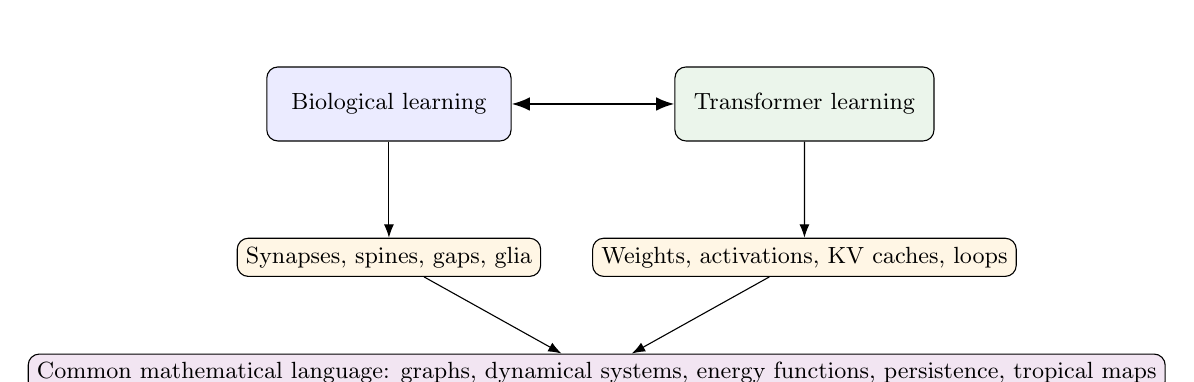
\begin{tikzpicture}[scale=0.94, transform shape, node distance=1.2cm, every node/.style={font=\small}, >=Latex]
\node[draw, rounded corners, fill=Blue!8, minimum width=3.3cm, minimum height=1cm] (bio) {Biological learning};
\node[draw, rounded corners, fill=Green!8, right=2.2cm of bio, minimum width=3.5cm, minimum height=1cm] (tfm) {Transformer learning};
\node[draw, rounded corners, fill=Orange!10, below=1.3cm of bio, minimum width=3.3cm] (syn) {Synapses, spines,\ gaps, glia};
\node[draw, rounded corners, fill=Orange!10, below=1.3cm of tfm, minimum width=3.5cm] (lat) {Weights, activations,\ KV caches, loops};
\node[draw, rounded corners, fill=Purple!10, below=1.3cm of $(syn)!0.5!(lat)$, minimum width=7.95cm] (math) {Common mathematical language: graphs, dynamical systems, energy functions, persistence, tropical maps};
\draw[->] (bio) -- (syn);
\draw[->] (tfm) -- (lat);
\draw[->] (syn) -- (math);
\draw[->] (lat) -- (math);
\draw[<->, thick] (bio) -- (tfm);
\end{tikzpicture}
\caption{Scope of the review. Biological and transformer systems are compared through explicit mathematical objects rather than through undisciplined metaphors.}
\label{fig:scope}
\end{figure}

\subsection{Terminological discipline}

The word \emph{learning} is overloaded. In neuroscience it often means an experience-dependent change in behavior mediated by physical modifications in neural and glial systems. At cellular resolution it may mean changes in synaptic strength, intrinsic excitability, dendritic integration, neuromodulatory set-points, receptor trafficking, structural connectivity, and gene expression. In machine learning it usually means optimization of parameters to reduce a loss over data. In transformer inference, people sometimes say the model \emph{learns in context}. This is computationally meaningful but physically different: the weights do not change; activations change. This manuscript therefore uses three terms.

\begin{definition}[Parameter learning, contextual adaptation, and state evolution]
\emph{Parameter learning} is a change in persistent parameters of a system: synaptic efficacies and biochemical states in biological circuits, or numerical weights in a neural network. \emph{Contextual adaptation} is task adaptation achieved by temporary internal states while persistent parameters are held fixed. \emph{State evolution} is the dynamical trajectory of voltage, calcium, hidden states, attention maps, or latent thoughts under fixed or slowly varying parameters.
\end{definition}

This distinction is central. Biological learning mixes all three. Transformer pretraining is parameter learning; ordinary inference is contextual adaptation and state evolution; latent and looped reasoning emphasizes state evolution; agentic systems add an external controller that chooses prompts, tools, searches, and memory retrieval operations.

\subsection{What counts as a valid analogy?}

An analogy is useful only when it preserves structure. The statement ``attention is like attention in the brain'' is usually too vague. A stronger statement is: scaled dot-product attention can be written as an associative memory retrieval rule with keys, queries, values, and an energy function; biological pattern completion in hippocampal circuits can also be modeled as associative memory; therefore both can be compared at the level of content-addressable retrieval, while differing in substrate, learning rule, timescale, and update locality. Similarly, the statement ``weights are synapses'' is only partly true. A transformer's weight matrix is a learned global tensor reused across token positions. A synapse is a local, stochastic, plastic, biochemical structure embedded in a living circuit, often with nonlinear dendritic consequences and neuromodulatory gating. The analogue is not identity; it is functional correspondence under a mathematical abstraction.

\begin{definition}[Structural analogy]
A structural analogy between systems $A$ and $B$ consists of objects $O_A,O_B$, operations $F_A,F_B$, and observables $Y_A,Y_B$ such that a map $\Phi:O_A\to O_B$ approximately preserves the operation-observable relation:
\[
Y_B(F_B(\Phi(o))) \approx \Psi(Y_A(F_A(o))).
\]
The analogy is weak if only surface words match, moderate if observables match, and strong if operations, invariants, and failure modes match.
\end{definition}

By this criterion, the strongest analogies in this review are: content-addressable retrieval; dynamical attractors; graph-based association; distributed coding; multiscale state-dependent plasticity; and energy or Lyapunov descriptions. The weakest analogies are: ``neurons as transformer tokens,'' ``synapses as static matrix entries,'' and ``chain-of-thought as human introspective reasoning.''

\section{Mathematical and physical preliminaries}

This section fixes notation and supplies the mathematics used later. The presentation is intentionally compact but self-contained enough to support the later theorems and comparisons.

\subsection{Graphs, hypergraphs, simplicial complexes, and language objects}

\begin{definition}[Typed directed multigraph]
A typed directed multigraph is a tuple
\[
G=(V,E,\tau_V,\tau_E,x_V,x_E),
\]
where $V$ is a finite set of vertices, $E\subseteq V\times V\times T_E$ is a multiset of typed directed edges, $\tau_V:V\to T_V$ gives vertex types, $\tau_E:E\to T_E$ gives edge types, and $x_V,x_E$ give node and edge features. In language applications, node types may include token, lemma, morpheme, root, syntactic phrase, semantic role, discourse entity, or latent thought; edge types may include next-token, dependency, constituency-parent, coreference, root-template-slot, entailment, or thought-dependency.
\end{definition}

\begin{definition}[Hypergraph and incidence representation]
A hypergraph is $H=(V,\mathcal{H})$ with hyperedges $h\in\mathcal{H}$ satisfying $h\subseteq V$. Its incidence graph is the bipartite graph with vertex set $V\cup\mathcal{H}$ and edges $(v,h)$ whenever $v\in h$. Hypergraphs are natural for predicate-argument structures, multi-token expressions, root-template morphology, and $k$-ary semantic relations.
\end{definition}

\begin{definition}[Abstract simplicial complex]
An abstract simplicial complex on a vertex set $V$ is a collection $K\subseteq 2^V$ such that if $\sigma\in K$ and $\tau\subseteq\sigma$, then $\tau\in K$. An element $\sigma$ with $|\sigma|=p+1$ is a $p$-simplex. Vertices are $0$-simplices, edges are $1$-simplices, triangles are $2$-simplices, and so on.
\end{definition}

A graph can be lifted to a simplicial complex by taking its clique complex: every clique becomes a simplex. A dependency tree has no cycles as a graph, but a semantic graph with coreference and discourse links may have cycles. A transformer layer applied to token embeddings supplies a weighted complete graph through attention; thresholding or filtrating that graph creates a family of complexes. The shape of such complexes can be measured by homology.

\begin{definition}[Vietoris-Rips filtration]
Let $X=\{x_1,\dots,x_n\}$ be points in a metric space with distance $d$. For scale $r\ge 0$, the Vietoris-Rips complex $\VR_r(X)$ contains a simplex $\sigma\subseteq X$ whenever $d(x_i,x_j)\le r$ for all $x_i,x_j\in\sigma$. The nested family $\{\VR_r(X)\}_{r\ge0}$ is the Vietoris-Rips filtration.
\end{definition}

Persistent topology tracks which homological features survive across $r$. In language embeddings, $X$ might be token embeddings at a layer, phrase embeddings, morpheme-root embeddings, or latent thought states. The distance $d$ might be Euclidean distance, cosine distance, attention-induced diffusion distance, or a learned metric.

\subsection{Boundary operators and homology}

Let $C_p(K)$ be the vector space over a field $\mathbb{F}$ generated by oriented $p$-simplices of $K$. The boundary map $\partial_p:C_p(K)\to C_{p-1}(K)$ is defined on an oriented simplex by
\[
\partial_p[v_0,\ldots,v_p]=\sum_{i=0}^p(-1)^i[v_0,\ldots,\widehat{v_i},\ldots,v_p].
\]
It satisfies $\partial_{p-1}\partial_p=0$. The $p$th homology group is
\[
H_p(K)=\ker \partial_p/\operatorname{im}\partial_{p+1}.
\]
Its dimension $\beta_p$ is the $p$th Betti number: $\beta_0$ counts connected components, $\beta_1$ counts independent loops, and $\beta_2$ counts voids.

\begin{lemma}[Boundary of a boundary is zero]
For every $p\ge 1$, $\partial_{p-1}\circ\partial_p=0$.
\end{lemma}
\begin{proof}
For a simplex $[v_0,\ldots,v_p]$, applying $\partial_p$ removes one vertex with sign $(-1)^i$. Applying $\partial_{p-1}$ removes a second vertex. Each ordered pair of removed vertices $i<j$ appears twice: once removing $i$ then $j$, and once removing $j$ then $i$. The two signs differ by a factor $-1$, so the terms cancel. Linearity completes the proof.
\end{proof}

In a language graph, $H_0$ features capture clustering or token-group formation; $H_1$ features can capture alternative relational routes, such as a word linked by syntax, semantics, and morphology to the same context; higher homology is harder to interpret but can indicate robust high-order relational cavities in embedding space. The interpretation is dataset- and metric-dependent; persistence gives invariant summaries, not semantic truth by itself.

\subsection{Distograms for language embeddings}

The term distogram is common in protein-structure prediction, where a model predicts a distribution over residue-residue distances. The same idea can be used for language embeddings.

\begin{definition}[Embedding distogram]
Given embeddings $z_1,\ldots,z_n\in\R^d$ and distance bins $0=b_0<b_1<\cdots<b_B$, an embedding distogram is a tensor
\[
D\in[0,1]^{n\times n\times B},\qquad \sum_{b=1}^B D_{ijb}=1,
\]
where $D_{ijb}$ estimates the probability that $d(z_i,z_j)\in[b_{b-1},b_b)$. Its expected distance matrix is
\[
\bar d_{ij}=\sum_{b=1}^B D_{ijb} c_b,
\]
where $c_b$ is a bin center. A deterministic distance matrix is the degenerate case in which each $D_{ij}$ is a point mass.
\end{definition}

For language models, a distogram can be obtained from raw embedding distances, from attention logits calibrated as similarities, from an auxiliary predictor, or from sampling multiple reasoning trajectories and measuring empirical distance distributions. A distogram supports uncertainty-aware filtrations: one can include an edge $(i,j)$ at scale $r$ when $\mathbb{P}(d(z_i,z_j)\le r)\ge q$ for confidence level $q$, or when $\E[d(z_i,z_j)]\le r$.

\subsection{Dynamical systems and energy}

A deterministic discrete-time dynamical system is $z_{t+1}=F(z_t)$ on state space $\calX$. A stochastic system is a Markov kernel $P(z,A)$ giving the probability of moving from state $z$ into measurable set $A$. Recurrent neural circuits, Hopfield networks, latent reasoning loops, and agentic graph-of-thought searches can all be analyzed as dynamical systems.

\begin{definition}[Lyapunov function]
For a discrete system $z_{t+1}=F(z_t)$, a Lyapunov function is a scalar $E:\calX\to\R$ such that $E(F(z))\le E(z)$ for all $z$, with strict inequality away from fixed points or invariant sets. In associative memory, $E$ is often called an energy.
\end{definition}

\begin{definition}[Ergodic Markov kernel]
A Markov kernel $P$ on a state space $\calX$ is ergodic with invariant distribution $\pi$ if $\pi P=\pi$ and for initial distributions $\mu$ in a specified class, $\mu P^t\to\pi$ as $t\to\infty$ in total variation, weak topology, or another specified metric.
\end{definition}

Ergodicity is relevant to stochastic reasoning loops: if a loop samples latent thoughts or graph expansions, then one can ask whether long-run samples explore a target distribution or collapse to attractors. Most current LLM agent loops have no formal ergodicity guarantee. GFlowNets are one route to a sampling objective with a mathematically specified terminal distribution.

\subsection{Tropical algebra and piecewise-linear neural maps}

\begin{definition}[Max-plus tropical semiring]
The max-plus tropical semiring is $(\R\cup\{-\infty\},\oplus,\otimes)$ with
\[
a\oplus b=\max(a,b),\qquad a\otimes b=a+b.
\]
The additive identity is $-\infty$ and the multiplicative identity is $0$.
\end{definition}

A tropical polynomial has the form
\[
f(x)=\bigoplus_{\alpha\in A} c_\alpha\otimes x^\alpha
=\max_{\alpha\in A}\{c_\alpha+\langle\alpha,x\rangle\}.
\]
It is a convex piecewise-linear function. Differences of such functions produce tropical rational maps. ReLU networks are piecewise-linear and can be represented in tropical terms under suitable constructions \cite{ZhangTropical2018,Brandenburg2024}. The softmax attention score
\[
\softmax(s/\tau)_i=\frac{\exp(s_i/\tau)}{\sum_j\exp(s_j/\tau)}
\]
approaches a hard max selector as $\tau\to0^+$. Thus low-temperature attention and max-plus dynamic programming are connected.

\begin{lemma}[Log-sum-exp tropical limit]
For $s\in\R^n$,
\[
\lim_{\tau\to0^+}\tau\log\sum_{i=1}^n \exp(s_i/\tau)=\max_i s_i.
\]
\end{lemma}
\begin{proof}
Let $m=\max_i s_i$. Then
\[
\tau\log\sum_i e^{s_i/\tau}=m+\tau\log\sum_i e^{(s_i-m)/\tau}.
\]
The sum inside the logarithm lies between $1$ and $n$, so the second term lies between $0$ and $\tau\log n$, which tends to $0$.
\end{proof}

\section{Biophysical learning in humans and mammals}

Human learning is not a single mechanism. Even a narrow memory task can involve hippocampal pattern separation, cortical association, prefrontal control, neuromodulatory reinforcement, cerebellar prediction, astrocyte metabolism, oligodendrocyte plasticity, and sleep-dependent consolidation. The following review focuses on cellular and molecular mechanisms most relevant for comparison with transformer learning: voltage dynamics, chemical synapses, electrical synapses and gap junctions, synaptic plasticity, biochemical cascades, engrams, and retrieval.

\subsection{Levels and timescales}

A useful first approximation is a stack of timescales.

\begin{longtable}{p{0.18\linewidth}p{0.25\linewidth}p{0.47\linewidth}}
\toprule
Scale & Typical time & Learning-relevant processes \\
\midrule
Ion-channel gating & microseconds to milliseconds & Action potentials, EPSPs/IPSPs, dendritic spikes, voltage-gated channel dynamics. \\
Synaptic transmission & milliseconds to seconds & Vesicle release, receptor binding, AMPA/NMDA/GABA conductances, short-term facilitation and depression. \\
Calcium signaling & milliseconds to minutes & NMDA-dependent calcium entry, CaMKII activation, calcineurin, PKA, MAPK, spine-local biochemical computation. \\
Early LTP/LTD & minutes to hours & AMPAR insertion/removal, phosphorylation, spine actin remodeling, presynaptic release changes. \\
Late LTP/consolidation & hours to days & Protein synthesis, CREB-dependent transcription, BDNF signaling, epigenetic regulation, engram stabilization. \\
Systems consolidation & days to years & Hippocampal-cortical redistribution, replay, schema formation, myelination and structural plasticity. \\
\bottomrule
\caption{Selected biological timescales relevant to learning. Exact times depend on species, brain region, cell type, age, and task.}
\end{longtable}

The transformer analogue spans different timescales: nanosecond-to-millisecond matrix operations; milliseconds-to-seconds decoding; minutes-to-days finetuning; weeks-to-months pretraining; persistent memory stored in parameter tensors and external retrieval stores. The biological system continuously updates itself during interaction with the world; the deployed transformer usually does not update its parameters unless explicitly trained or equipped with a memory-writing subsystem.

\subsection{Conductance-based neurons}

The membrane potential $V$ of a small isopotential neuron patch can be modeled by a capacitance equation
\[
C_m\frac{dV}{dt}= -\sum_k g_k(t,V)(V-E_k) + I_{\rm syn}(t)+I_{\rm ext}(t),
\]
where $C_m$ is membrane capacitance, $g_k$ are ion-channel conductances, $E_k$ are reversal potentials, and $I_{\rm syn}$ contains chemical and electrical synaptic currents. The Hodgkin-Huxley model writes sodium and potassium conductances as voltage-dependent gating variables. A reduced integrate-and-fire model writes
\[
\tau_m\frac{dV}{dt}=-(V-E_L)+R_m I(t),
\]
with a reset rule when $V$ reaches threshold.

The physical difference from an artificial unit is substantial. A biological neuron has dendritic compartments, nonlinear synaptic integration, active dendritic spikes, spatial cable filtering, stochastic channel noise, local protein synthesis, and synapse-specific biochemical state. An artificial transformer neuron is an algebraic coordinate in a vector operation. Yet, at a high level, both are nonlinear maps from inputs to outputs, and both can support distributed representation when many units interact.

\subsection{Chemical synapses and local plasticity}

At a chemical synapse, an action potential opens presynaptic calcium channels, calcium triggers vesicle fusion, neurotransmitter crosses the cleft, postsynaptic receptors change conductance, and intracellular signaling modifies future transmission. A conductance-based excitatory synaptic current can be written
\[
I_{ij}^{\rm chem}(t)=g_{ij}(t)s_{ij}(t)(V_i(t)-E_{\rm exc}),
\]
where $s_{ij}$ is a gating variable driven by presynaptic spikes and receptor kinetics. Inhibitory synapses have different reversal potentials and receptor kinetics.

Synaptic weight is therefore not a single scalar in the biological substrate. A practical scalar efficacy $w_{ij}$ may summarize several factors:
\[
w_{ij}\approx N_{\rm release\ sites}\,p_{\rm release}\,q_{\rm vesicle}\,N_{\rm AMPAR}\,\gamma_{\rm AMPAR}\,F_{\rm dendrite},
\]
where $F_{\rm dendrite}$ captures dendritic location and active conductances. Plasticity can alter any factor. This already differs from a transformer weight entry, which is a scalar parameter in a matrix shared over positions and updated by global gradient descent.

\subsection{Spike-timing-dependent plasticity and Hebbian structure}

Hebbian learning is often paraphrased as correlated activity strengthening a connection. A more precise family of rules is spike-timing-dependent plasticity (STDP). A basic pair-based rule is
\[
\Delta w =
\begin{cases}
A_+\exp(-\Delta t/\tau_+), & \Delta t=t_{\rm post}-t_{\rm pre}>0,\\
-A_-\exp(\Delta t/\tau_-), & \Delta t<0.
\end{cases}
\]
Pre-before-post spike pairs tend to potentiate, while post-before-pre pairs tend to depress, though real plasticity rules depend on cell type, developmental stage, dendritic voltage, neuromodulators, firing rate, and inhibitory/excitatory context \cite{Markram1997,BiPoo1998,Sjostrom2008}. The rule is local in the sense that it depends on pre- and postsynaptic activity and local state, but global behavioral relevance can gate plasticity through dopamine, acetylcholine, norepinephrine, serotonin, and other signals.

\begin{proposition}[STDP as a local temporal-correlation estimator]
For stationary pre- and postsynaptic point processes with cross-correlation $C_{pre,post}(\Delta)$, the expected infinitesimal weight change under a pair-based STDP kernel $K(\Delta)$ is proportional to
\[
\E[\Delta w]\propto \int_{-\infty}^{\infty} K(\Delta)C_{pre,post}(\Delta)d\Delta.
\]
\end{proposition}
\begin{proof}
The expected number of pre-post spike pairs with lag $\Delta$ in a long observation window is proportional to the cross-correlation density $C_{pre,post}(\Delta)$. The STDP rule adds $K(\Delta)$ for each such pair. Integrating over lags gives the expectation up to observation-time and rate constants.
\end{proof}

The transformer analogue is not backpropagation. Backpropagation computes exact or stochastic gradients of a global objective through many layers. STDP estimates local temporal correlations. There are machine-learning rules inspired by Hebbian updates, contrastive learning, predictive coding, equilibrium propagation, and three-factor learning, but a standard transformer is not trained by STDP.

\subsection{NMDA receptors, AMPA trafficking, and calcium-dependent plasticity}

A canonical excitatory LTP mechanism in hippocampal CA1 begins when glutamatergic synaptic input depolarizes the postsynaptic spine enough to relieve the magnesium block of NMDA receptors. NMDA receptors then allow calcium influx. Calcium concentration and time course influence whether kinases or phosphatases dominate. Large, brief calcium elevations tend to activate CaMKII and support LTP; smaller, longer elevations tend to activate phosphatases and support LTD. This simplified threshold picture is not universal but remains useful.

CaMKII is central because it is abundant in excitatory synapses, activated by calcium/calmodulin, capable of autophosphorylation and structural interactions, and linked to AMPAR trafficking and synaptic strength. Recent reviews emphasize both kinase activity and scaffolding/structural roles, including binding to NMDA receptor subunits such as GluN2B \cite{Hayashi2022,Nicoll2023,Bayer2025}. AMPA receptor insertion increases postsynaptic response; AMPAR endocytosis decreases it. Plasticity also involves actin remodeling, spine enlargement or shrinkage, trans-synaptic adhesion molecules, local translation, and protein degradation.

A minimal calcium-control model writes
\[
\frac{dw}{dt}=\eta_+\phi_+(C)(w_{\max}-w)-\eta_-\phi_-(C)(w-w_{\min}),
\]
where $C$ is spine calcium, $\phi_+$ and $\phi_-$ are activation functions for potentiating and depressing pathways, and $w$ is an effective synaptic efficacy. This equation is useful as a mathematical abstraction but hides many molecular states.

\begin{figure}[H]
\centering
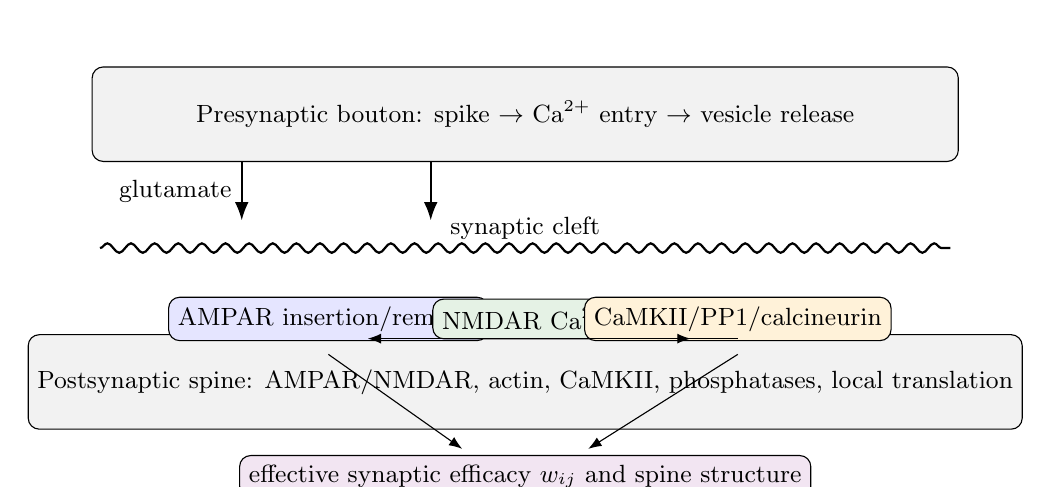
\begin{tikzpicture}[every node/.style={font=\small}, >=Latex]
\node[draw, rounded corners, fill=gray!10, minimum width=11cm, minimum height=1.2cm] (pre) at (0,3.4) {Presynaptic bouton: spike $\to$ Ca$^{2+}$ entry $\to$ vesicle release};
\node[draw, rounded corners, fill=gray!10, minimum width=11cm, minimum height=1.2cm] (post) at (0,0) {Postsynaptic spine: AMPAR/NMDAR, actin, CaMKII, phosphatases, local translation};
\draw[decorate,decoration={snake,amplitude=0.6mm,segment length=3mm}, thick] (-5.4,1.7) -- (5.4,1.7);
\node at (0,1.95) {synaptic cleft};
\draw[->, thick] (-3.6,2.8) -- (-3.6,2.05) node[midway,left] {glutamate};
\draw[->, thick] (-1.2,2.8) -- (-1.2,2.05);
\node[draw, fill=Blue!10, rounded corners] at (-2.5,0.8) {AMPAR insertion/removal};
\node[draw, fill=Green!10, rounded corners] at (0,0.8) {NMDAR Ca$^{2+}$};
\node[draw, fill=Orange!15, rounded corners] at (2.7,0.8) {CaMKII/PP1/calcineurin};
\draw[->] (0,0.55) -- (2.1,0.55);
\draw[->] (2.7,0.55) -- (-2.0,0.55);
\node[draw, fill=Purple!10, rounded corners] at (0,-1.2) {effective synaptic efficacy $w_{ij}$ and spine structure};
\draw[->] (-2.5,0.35) -- (-0.8,-0.85);
\draw[->] (2.7,0.35) -- (0.8,-0.85);
\end{tikzpicture}
\caption{Original schematic of a chemical synapse and molecular plasticity. A scalar synaptic weight is an abstraction over many physical and biochemical degrees of freedom.}
\label{fig:chemical_synapse}
\end{figure}

\subsection{Gap junctions and electrical synapses}

Gap junctions are intercellular channels formed by connexins. In neurons, connexin 36 (Cx36) is especially important for electrical synapses. Two hemichannels align across adjacent membranes, permitting direct passage of ions and small molecules; this creates fast electrical coupling. Astrocytes prominently express connexins such as Cx43 and Cx30 and form large coupled networks that redistribute ions and metabolites and modulate neuronal activity. Recent work continues to show that astrocytic gap junction networks are not passive plumbing; they can influence hippocampal network activity, synaptic plasticity, development, and memory-relevant processes \cite{LeeCx36Structure2023,Dossi2024,Asher2025,Cooper2026}.

For two electrically coupled cells $i$ and $j$, the gap-junction current into $i$ is often modeled as
\[
I_{ij}^{\rm gap}=g_{ij}^{\rm gap}(V_j-V_i),
\]
where $g_{ij}^{\rm gap}$ is gap-junction conductance. For a network,
\[
C_i\dot V_i=F_i(V_i,\ldots)+\sum_j g_{ij}^{\rm gap}(V_j-V_i).
\]
The coupling term is a graph Laplacian. If $G=(g_{ij})$ is symmetric and $L$ is its weighted Laplacian, then the electrical coupling contributes $-LV$ to voltage dynamics.

\begin{lemma}[Gap-junction Laplacian dissipates voltage variance]
Assume identical capacitances and pure symmetric electrical coupling $\dot V=-LV$ on a connected weighted graph. Let $\bar V=n^{-1}\sum_i V_i$ and $\mathcal{V}(V)=\frac12\sum_i(V_i-\bar V)^2$. Then $\bar V$ is constant and
\[
\frac{d}{dt}\mathcal{V}(V)=-V^\top L V=-\frac12\sum_{i,j}g_{ij}(V_i-V_j)^2\le0.
\]
Thus electrical coupling synchronizes voltages in the absence of other currents.
\end{lemma}
\begin{proof}
Since $L\1=0$, $d\bar V/dt=-n^{-1}\1^\top LV=0$. With $V$ replaced by $V-\bar V\1$, the derivative of variance is $(V-\bar V\1)^\top\dot V=-V^\top L V$. The quadratic identity for a graph Laplacian gives the final expression. Connectedness implies the only zero-variance equilibrium is consensus.
\end{proof}

This lemma is a concrete example of a strong analogy: gap-junction coupling, graph diffusion, attention diffusion, and Laplacian smoothing all use graph operators. But the substrate and semantics differ. Gap junctions directly couple membrane voltages and metabolites; attention computes data-dependent weighted averages of value vectors.

\subsection{Astrocytes, metabolism, and non-neuronal learning contributions}

The older neuron-centric view is incomplete. Astrocytes regulate extracellular potassium, neurotransmitter uptake, lactate shuttling, blood flow, synaptogenesis, and gliotransmission. They can respond to neuronal activity with calcium signals and modulate synapses. Astrocytic gap junction networks can coordinate activity across local tissue, and recent reviews emphasize astrocytes as active participants in memory processes \cite{Escalada2024,Asher2025,Alberini2025}. Oligodendrocytes and myelin plasticity contribute to timing and circuit efficiency. Microglia remodel synapses and participate in development and disease. These facts matter for transformer comparisons because a biological memory system is not merely a graph of neurons; it is a graph of multiple cell types and biochemical reservoirs.

An artificial model with external memory, retrieval-augmented generation, tool use, and agentic controllers is therefore more analogous to a coupled ecosystem than to a single recurrent neural network. But again the analogy is structural, not biological: astrocytic lactate shuttling is not a vector database, and a vector database is not glia. Both can be modeled as auxiliary support systems that modulate what computations are available and when.

\subsection{Engrams, pattern separation, and pattern completion}

A memory engram is a physical ensemble and set of modifications that can support memory recall when reactivated. Modern engram studies use activity-dependent labeling, optogenetics, chemogenetics, calcium imaging, and single-cell methods to identify and manipulate memory-associated cells. The field has moved beyond a rigid view in which a memory is stored in a fixed set of cells. Recent work emphasizes overlap, linking, competition, inhibitory plasticity, turnover, and dynamic engram states \cite{Josselyn2015,Tonegawa2015,Choucry2024,Tome2024,Zaki2025,Eom2025,Sung2026}.

Hippocampal pattern separation and pattern completion are especially relevant to associative memory. Dentate gyrus and CA3 circuitry can help map similar inputs to distinct representations and retrieve stored patterns from partial cues. This resembles Hopfield-style associative memory at a mathematical level, but biological retrieval is embedded in oscillations, neuromodulation, synaptic heterogeneity, adult neurogenesis, inhibition, and hippocampal-cortical interactions.

\subsection{Biochemical memory is distributed and partially redundant}

A synapse can store traces in receptor state, scaffold composition, spine volume, presynaptic release machinery, local mRNA availability, mitochondrial positioning, and extracellular matrix. A circuit can store traces in connectivity patterns, inhibitory balance, recurrent attractors, oscillatory coupling, and systems-level engram allocation. This redundancy is one reason biological memory can be robust to noise and partial damage. It also means there is no one-to-one counterpart of a matrix parameter.

\begin{remark}[The word ``weight'' hides different physics]
A transformer's weight entry $W_{ab}$ is a numerical parameter used in a multiply-add operation. A biological synaptic weight is an effective observable resulting from many stochastic molecular and morphological variables. A gap-junction conductance is a physical channel conductance coupling voltages. These can all be abstracted as edge weights in a graph, but that abstraction discards mechanism.
\end{remark}

\section{Transformer learning, memory, and latent reasoning}

\subsection{The standard transformer block}

Let $X\in\R^{n\times d}$ be a sequence of $n$ token representations. For one attention head,
\[
Q=XW_Q,
\quad K=XW_K,
\quad V=XW_V,
\quad A=\softmax\left(\frac{QK^\top}{\sqrt{d_k}}+B\right),
\quad Y=AV,
\]
where $B$ may encode causal masking or positional bias. Multi-head attention concatenates several $Y_h$ and projects them. A transformer block applies residual connections, layer normalization, and an MLP:
\[
X_{\ell+1}=X_\ell+\operatorname{MHA}(\operatorname{LN}(X_\ell)),
\quad
X_{\ell+1}=X_{\ell+1}+\operatorname{MLP}(\operatorname{LN}(X_{\ell+1})).
\]
A decoder-only language model predicts the next token distribution by
\[
p_\theta(x_{t+1}\mid x_{\le t})=\softmax(W_U h_t)_x.
\]
The parameters $\theta$ are learned by minimizing cross-entropy over a corpus:
\[
\min_\theta -\sum_{(x_1,\dots,x_T)}\sum_{t=1}^{T-1}\log p_\theta(x_{t+1}\mid x_{\le t}).
\]

\subsection{What is stored where?}

A trained transformer stores different information in different structures. Token embeddings store lexical and subword coordinates; attention and MLP matrices store reusable feature transformations; layer norms set scale; positional encodings or relative position mechanisms help represent order; KV caches store temporary per-context keys and values; external retrieval systems store documents or facts outside the model; adapters store task-specific low-rank updates. None of these is identical to biological memory, but several analogies are useful.

\begin{longtable}{p{0.22\linewidth}p{0.35\linewidth}p{0.34\linewidth}}
\toprule
Transformer object & Function & Biological analogue and caveat \\
\midrule
Embedding vector & Coordinate for token/subword/state & Population code; caveat: learned static table or computed activation, not a living neural population. \\
Attention key & Address used for retrieval & Cue representation in associative memory; caveat: vector dot-product address, not hippocampal/cortical dynamics. \\
Attention value & Retrieved content & Retrieved pattern/content; caveat: value is a linear projection of activations. \\
Parameter matrix & Persistent learned transformation & Synaptic/circuit efficacy; caveat: global tensor updated by backprop, not local biochemical synapse. \\
KV cache & Temporary contextual memory & Working memory or active trace; caveat: exact stored activations with finite context window. \\
Residual stream & Shared state channel across layers & Distributed neural state; caveat: artificial layer-indexed computation. \\
Latent loop & Iterative state evolution & Recurrent circuit dynamics; caveat: engineered loop with fixed weights. \\
External vector DB & Retrieved documents or memories & Episodic/semantic support systems; caveat: discrete engineered memory store. \\
\bottomrule
\caption{Transformer memory objects and cautious biological analogues.}
\end{longtable}

\subsection{Attention as associative memory}

Modern Hopfield-network theory shows that a continuous associative memory update can be written in a form equivalent to attention \cite{Ramsauer2021}. Given stored patterns as keys $K$ and values $V$, and a query $q$, attention returns
\[
y=\sum_i \frac{\exp(\beta q^\top k_i)}{\sum_j\exp(\beta q^\top k_j)}v_i.
\]
For high inverse temperature $\beta$, this approaches nearest-pattern retrieval; for low $\beta$, it averages broadly. Transformer heads can therefore be interpreted as content-addressable retrieval modules.

\begin{theorem}[Attention-Hopfied retrieval equivalence, simplified]
Let stored key-value pairs be $(k_i,v_i)_{i=1}^n$ and let the energy of a query state $q$ be
\[
E(q)=-\beta^{-1}\log\sum_{i=1}^n \exp(\beta q^\top k_i)+\frac12\|q\|^2.
\]
The negative gradient of the log-sum-exp term yields a softmax-weighted combination of keys. If values equal stored patterns or a learned projection of them, the retrieval update is mathematically the same softmax attention operation used in transformers.
\end{theorem}
\begin{proof}
Differentiating gives
\[
\nabla_q \left(\beta^{-1}\log\sum_i e^{\beta q^\top k_i}\right)=\sum_i \frac{e^{\beta q^\top k_i}}{\sum_j e^{\beta q^\top k_j}}k_i.
\]
Replacing $k_i$ by associated values $v_i$ through a value matrix gives the usual attention readout. The full Hopfield update includes details of the state map and energy normalization, but the core retrieval operation is the same softmax-weighted association.
\end{proof}

This theorem supports a strong mathematical analogy with associative memory. It does not imply that transformer attention implements hippocampal physiology. Biological associative memory can use recurrent excitation, inhibition, sparse coding, dendritic nonlinearities, synaptic plasticity, and oscillations; attention uses matrix multiplication and softmax.

\begin{figure}[H]
\centering
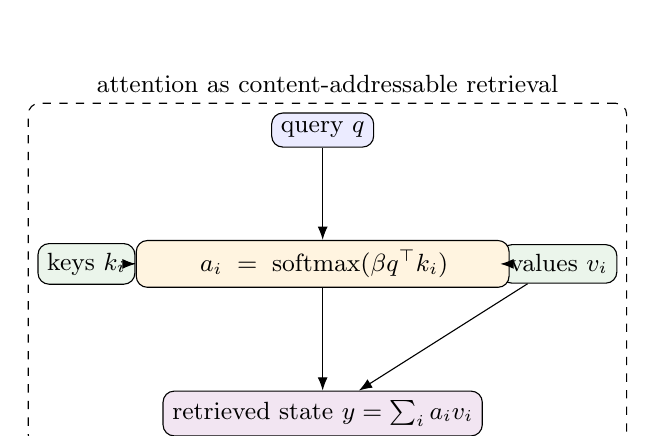
\begin{tikzpicture}[every node/.style={font=\small}, >=Latex]
\node[draw, rounded corners, fill=Blue!8] (q) at (0,2.5) {query $q$};
\node[draw, rounded corners, fill=Green!8] (k) at (-3,0.8) {keys $k_i$};
\node[draw, rounded corners, fill=Green!8] (v) at (3,0.8) {values $v_i$};
\node[draw, rounded corners, fill=Orange!12, text width=4.5cm, align=center] (s) at (0,0.8) {$a_i=\softmax(\beta q^\top k_i)$};
\node[draw, rounded corners, fill=Purple!10] (y) at (0,-1.1) {retrieved state $y=\sum_i a_i v_i$};
\draw[->] (q) -- (s);
\draw[->] (k) -- (s);
\draw[->] (s) -- (v);
\draw[->] (v) -- (y);
\draw[->] (s) -- (y);
\node[draw, rounded corners, dashed, fit=(q)(k)(v)(s)(y), label={[font=\small]above:attention as content-addressable retrieval}] {};
\end{tikzpicture}
\caption{Original schematic of attention as associative memory retrieval. The same equation can be read as a transformer attention head or as a modern Hopfield retrieval step.}
\label{fig:hopfield_attention}
\end{figure}

\subsection{Parameter learning versus in-context learning}

A transformer trained by gradient descent updates parameters according to
\[
\theta_{t+1}=\theta_t-\eta_t \widehat\nabla_\theta \mathcal{L}(\theta_t;B_t),
\]
where $B_t$ is a minibatch. This is global credit assignment through backpropagation. In-context learning, by contrast, keeps $\theta$ fixed and maps a prompt containing examples to a prediction:
\[
y=F_\theta((x_1,y_1),\dots,(x_m,y_m),x_*) .
\]
Several theoretical and empirical works show that transformers can implement learning-like algorithms in-context, including regression-like procedures or induction heads \cite{Olsson2022,Akyurek2023,VonOswald2023,Garg2022,Smart2025}. But this is not persistent learning unless the prompt or an external memory is preserved.

A useful biological comparison is working memory or active cortical state, not synaptic consolidation. A human can use context to infer a new word meaning without immediately forming a stable memory; later consolidation may stabilize the association. Similarly, a transformer can infer a temporary mapping from a prompt; once the context is gone, the base model has not changed.

\subsection{Latent and looped reasoning}

Chain-of-thought prompting exposes intermediate reasoning in natural language tokens. Latent reasoning methods ask whether some intermediate computation should occur in hidden states rather than surface words. Coconut feeds the last hidden state back as a continuous thought token, allowing hidden-state trajectories that need not decode into text at each step \cite{Hao2024}. SoftCoT and SoftCoT++ use soft thought tokens and projection modules to supply continuous reasoning information to an LLM without necessarily modifying the whole backbone \cite{SoftCoT2025,SoftCoTPlus2025}. Looped transformer work studies recurrence over transformer blocks, allowing a fixed parameter set to apply multiple iterative computation steps; recent latent-reasoning surveys and looped language model preprints present this as a scaling direction for inference-time computation \cite{YangLooped2024,Saunshi2025,ZhuLatentSurvey2025,ZhuOuro2025}.

Mathematically, a latent reasoning loop can be written
\[
z_{t+1}=F_\theta(z_t,x,u_t),\qquad y_t=G_\theta(z_t),
\]
where $x$ is the problem context and $u_t$ may include a controller action, sampled thought expansion, retrieval result, or tool output. If $u_t$ is stochastic, this is a Markov decision process or controlled Markov chain in embedding space.

\subsection{Graph-of-thought and agentic reasoning}

Graph-of-Thoughts (GoT) treats LLM-generated thoughts as vertices and dependencies or transformations as edges. Unlike a chain, a graph can merge, refine, aggregate, critique, backtrack, and recombine thoughts \cite{BestaGoT2023,GraphThoughtsSurvey2024}. Agentic systems add tools, retrieval, verifiers, planners, and sometimes multiple models. The relevant learning-like process is inference-time search over a structured state space.

This resembles biological recurrence more than one-pass decoding, but the analogy remains limited. Biological recurrence is continuous, embodied, and learned over a lifetime. Agentic recurrence is usually engineered by prompts and external program logic. Still, graph-of-thought reasoning provides a natural interface with TokenGT: thoughts are graph nodes, dependencies are edges, and latent thought vectors can be processed by the same graph-tokenized transformer.

\subsection{GFlowNets for diverse reasoning trajectories}

A Generative Flow Network (GFlowNet) learns a policy that samples compositional objects with probability proportional to a reward $R(x)$, rather than only maximizing reward. In a directed acyclic state graph with source $s_0$, forward policy $P_F$, backward policy $P_B$, and terminal object $x$, the trajectory-balance objective enforces
\[
\log Z + \sum_{t=0}^{T-1}\log P_F(s_{t+1}\mid s_t)
=\log R(x)+\sum_{t=0}^{T-1}\log P_B(s_t\mid s_{t+1}).
\]
Continuous GFlowNets generalize this idea to continuous or hybrid spaces under measure-theoretic assumptions \cite{BengioGFlowNet2021,Lahlou2023,Brunswic2023,Younsi2025}. For reasoning, a state can be a partial thought graph, a latent embedding state, or a graph plus natural-language commitments. A reward can be supplied by a verifier, proof checker, process reward model, consistency metric, or human feedback.

\begin{theorem}[Trajectory balance gives reward-proportional terminal sampling]
In a finite acyclic GFlowNet state graph, suppose every complete trajectory $\tau:s_0\to x$ satisfies the trajectory-balance equation above. Then the terminal distribution induced by $P_F$ satisfies
\[
P_F(x)=\frac{R(x)}{Z}.
\]
\end{theorem}
\begin{proof}
Rearranging trajectory balance gives
\[
\prod_t P_F(s_{t+1}\mid s_t)=\frac{R(x)}{Z}\prod_t P_B(s_t\mid s_{t+1}).
\]
Summing over all trajectories ending at $x$, the backward trajectory probabilities from $x$ to $s_0$ sum to $1$ under a valid backward policy on the acyclic graph. Therefore $P_F(x)=\sum_{\tau:s_0\to x}P_F(\tau)=R(x)/Z$.
\end{proof}

For language reasoning, this theorem is attractive because one often wants diverse high-quality solution paths, not only the single highest-reward path. A continuous latent GFlowNet could sample embedding-space thought trajectories and graph expansions proportional to verifier reward, while TokenGT supplies graph-structured state representation.

\section{Precise comparison of biological and transformer learning}

\subsection{The substrate contrast}

Biological learning is local, embodied, asynchronous, chemically mediated, and metabolically constrained. Transformer learning is usually centralized, batched, synchronous, differentiable, and optimized against a scalar loss. Biological neurons update while acting in the world; transformer parameters are usually frozen during deployment. Biological memories are stored in living tissue with multiple redundant mechanisms; transformer memories are stored in floating-point tensors and external data structures.

Nevertheless, both systems instantiate high-dimensional dynamical computation. Both use distributed codes. Both retrieve information by partial cues. Both can exhibit attractor-like behavior. Both compress experience into persistent structures. Both can produce compositional generalization, and both fail in ways related to distribution shift, interference, spurious correlations, and overconfident retrieval.

\subsection{Information storage}

In a biological circuit, storage can be written abstractly as a change in a parameter-and-state field
\[
\mathcal{M}_{bio}=(W_{chem},G_{gap},\Theta_{ion},S_{spine},M_{glia},R_{receptor},E_{gene},\ldots),
\]
where $W_{chem}$ are chemical synaptic efficacies, $G_{gap}$ gap-junction conductances, $\Theta_{ion}$ intrinsic excitability parameters, $S_{spine}$ structural spine variables, $M_{glia}$ glial/metabolic variables, $R_{receptor}$ receptor states, and $E_{gene}$ transcriptional/epigenetic variables. This state is plastic across many timescales.

In a transformer, persistent storage is roughly
\[
\mathcal{M}_{tfm}=(E_{tok},E_{pos},W_Q,W_K,W_V,W_O,W_{MLP},\gamma,\beta,W_U,\ldots),
\]
plus optional adapters, retrieval indices, system prompts, and memory databases. Temporary inference storage is
\[
\mathcal{S}_{tfm}(x)=(X_0,X_1,\ldots,X_L,K_{cache},V_{cache},A_1,\ldots,A_L,z_{loop},\ldots).
\]
A deployed transformer's temporary state may be large and useful, but it is normally discarded after the session unless written externally.

\subsection{Retrieval}

Biological retrieval can be cue-driven: a partial cue activates a network that reinstates an engram or reconstructs a memory. Retrieval is state-dependent: mood, context, neuromodulation, sleep, stress, and competing memories matter. Transformer retrieval is prompt-driven: tokens generate activations, attention selects context, and output logits produce a distribution. Retrieval-augmented generation adds external nearest-neighbor search.

The strongest shared formalism is content-addressable memory. Let stored patterns be $\xi_1,\ldots,\xi_m$. Classical Hopfield retrieval evolves a state toward an attractor. Transformer attention retrieves a weighted average of values. Hippocampal pattern completion retrieves through recurrent circuitry. In all cases, a cue induces movement toward stored or constructed content.

\subsection{Associative memory and interference}

Associative memory has a capacity-interference tradeoff. Classical Hopfield networks have limited capacity under random dense binary patterns; modern dense associative memories and attention-like updates can have much larger capacity in high-dimensional continuous spaces \cite{Hopfield1982,KrotovHopfield2016,Ramsauer2021}. Biological systems use sparse coding, inhibition, adult neurogenesis, synaptic consolidation, and hippocampal-cortical separation to manage interference. Transformers use high dimensionality, attention, MLP superposition, scale, data diversity, and optimization. Mechanistic interpretability shows that features may be stored in superposition, with circuits such as induction heads contributing to in-context pattern completion \cite{Elhage2021,Olsson2022,Crosbie2025}.

\subsection{Credit assignment}

Backpropagation computes gradients using a global computational graph. Biological credit assignment is unresolved as a complete theory. Candidate mechanisms include local Hebbian rules, three-factor learning rules with neuromodulatory signals, dendritic prediction errors, feedback alignment-like processes, predictive coding, equilibrium propagation, and reinforcement learning through basal ganglia loops. No evidence shows that the brain literally performs standard backpropagation through deep transformer-like layers. Conversely, no standard transformer implements the full biochemical richness of biological plasticity.

\subsection{Gap junction analogues in transformers}

Gap junctions are not attention. They are physical channels that directly couple cells. The best mathematical analogues are Laplacian diffusion, residual mixing, synchronization coupling, and graph smoothing. In transformer systems, one might compare gap junction coupling to:

\begin{enumerate}
\item residual stream sharing, because information flows directly across layers;
\item attention diffusion, because each token mixes with others by weighted averaging;
\item graph neural Laplacian smoothing, because states are coupled over edges;
\item latent loop synchronization, because repeated updates can converge to shared fixed points;
\item multi-agent communication channels, because agents may exchange hidden or natural-language state.
\end{enumerate}

The analogy is mathematical only. Gap junctions have conductance, gating, connexin composition, rectification, and biochemical permeability. Transformer mixing has dot-product similarity, softmax normalization, learned projections, and numerical precision.

\subsection{A compact comparison table}

\begin{longtable}{p{0.18\linewidth}p{0.35\linewidth}p{0.35\linewidth}}
\toprule
Dimension & Human/mammalian learning & Transformer/agentic latent learning \\
\midrule
Persistent storage & Synapses, spines, receptors, intrinsic excitability, glia, gene expression, systems consolidation & Parameter matrices, embeddings, adapters, retrieval stores, prompts, tool memories \\
Update rule & Local biochemical plasticity, neuromodulatory gating, structural remodeling, replay/consolidation & Backpropagation, RLHF/RLAIF, supervised finetuning, adapters; during inference often fixed weights \\
Temporary state & Membrane voltage, calcium, oscillations, working memory, neuromodulatory state & Residual stream, hidden activations, KV cache, latent thought vectors, tool state \\
Associative retrieval & Hippocampal/cortical pattern completion, engram reactivation & Attention/Hopfield retrieval, nearest-neighbor retrieval, in-context induction \\
Graph structure & Connectome, synaptic graph, gap-junction graph, astrocyte network, functional connectivity & Token graph, attention graph, dependency/semantic graph, thought graph, retrieval graph \\
Timescale & milliseconds to lifetime & inference milliseconds/seconds; training hours/months; external memory persistent if saved \\
Noise & Stochastic spiking, molecular noise, sensory uncertainty & Sampling temperature, numerical noise, dropout during training, stochastic decoding \\
Energy and metabolism & ATP, ion gradients, mitochondrial and vascular support & FLOPs, memory bandwidth, accelerator energy, latency \\
Interpretability & Measurable but invasive; causal manipulation possible in animals & Weight/activation analysis, circuits, probes, sparse autoencoders, but opaque at scale \\
Main caveat & Not reducible to scalar synaptic weights & Not biologically local; no embodied biochemical substrate \\
\bottomrule
\caption{High-level comparison between biological and transformer learning.}
\end{longtable}

\section{Language as graph-structured information}

\subsection{Why string order is insufficient}

Autoregressive language models are trained on strings. But strings are projections of richer relational objects. Consider the sentence ``The scientist who the students quoted revised the theorem.'' Linear order alone obscures subject-verb relations, relative clause structure, and semantic roles. A dependency parse supplies edges such as scientist--revised and students--quoted; a constituency parse supplies nested phrases; semantic role labeling supplies predicate-argument frames; coreference links connect mentions; morphology links surface words to lemmas and affixes. These relations are graph-structured.

Treating language as a graph does not mean discarding order. It means making order one edge type among many. A useful language graph for a document can contain:
\[
V=V_{tok}\cup V_{lemma}\cup V_{morph}\cup V_{phrase}\cup V_{entity}\cup V_{predicate}\cup V_{thought},
\]
with edges for adjacency, dependency, constituency, lemma membership, morphological decomposition, coreference, discourse, entailment, and reasoning dependencies.

\subsection{TokenGT recap}

TokenGT starts from a simple observation: a standard transformer can process a graph if nodes and edges are turned into tokens with appropriate embeddings. In TokenGT, node tokens and edge tokens are fed to a pure transformer. Orthogonal or orthogonally initialized vertex identifiers, edge identifiers, endpoint identifiers, and type identifiers help encode incidence structure. The original work proves that with suitable token embeddings, the model is at least as expressive as a 2-invariant graph network and can be extended to higher-order hypergraphs \cite{KimTokenGT2022}. This is important because it separates graph representation from graph-specific attention machinery. The attention operator remains standard.

For language, a TokenGT input sequence might be:
\[
[\text{node: token}_1,\ldots,\text{node: token}_n,\text{edge: dep}_{i,j},\text{edge: coref}_{p,q},\ldots].
\]
Each edge token encodes its endpoints, relation type, and features. Hyperedges can be represented by hyperedge tokens connected through incidence identifiers.

In implementation, vertex identity, edge identity, and endpoint incidence should be separate structural channels. For a graph with \(n\) vertices and \(m\) edge tokens, vertex identifiers occupy one range, edge identifiers occupy a disjoint range, and each edge token also carries the pair of endpoint vertex identifiers. Exact pairwise orthogonality is possible only when the identifier embedding dimension is at least the number of active identifiers; otherwise the practical substitute is an orthogonally initialized or hash-signed identifier table whose collisions are controlled by graph-size caps.

\begin{figure}[H]
\centering
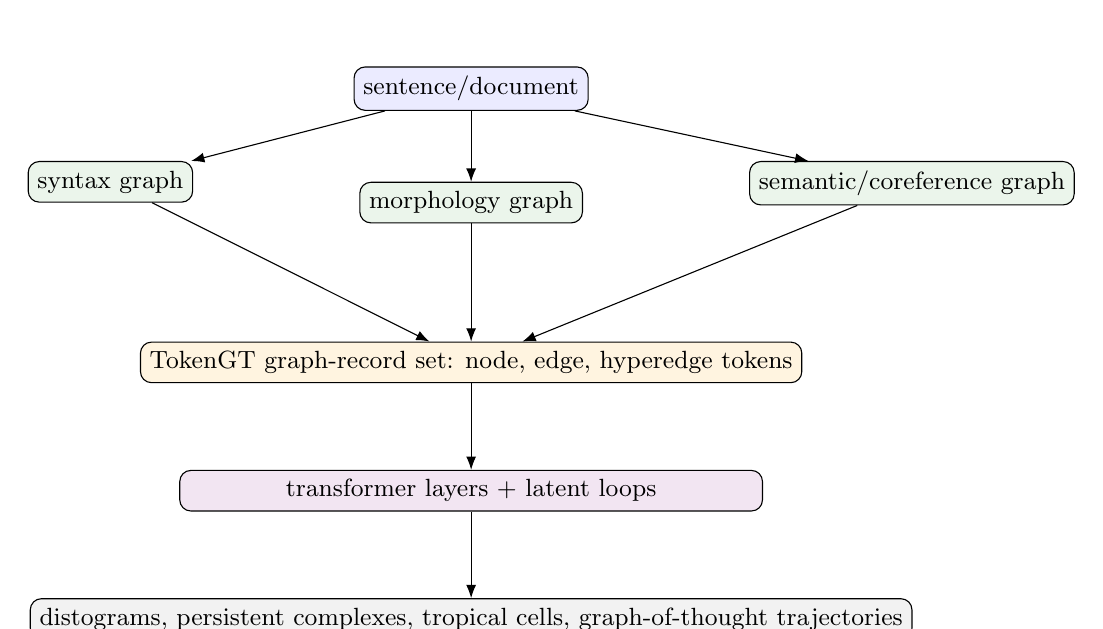
\begin{tikzpicture}[every node/.style={font=\small}, >=Latex, node distance=0.9cm]
\node[draw, rounded corners, fill=Blue!8] (sent) {sentence/document};
\node[draw, rounded corners, fill=Green!8, below left=of sent, xshift=-1.4cm] (parse) {syntax graph};
\node[draw, rounded corners, fill=Green!8, below=of sent] (morph) {morphology graph};
\node[draw, rounded corners, fill=Green!8, below right=of sent, xshift=1.4cm] (sem) {semantic/coreference graph};
\node[draw, rounded corners, fill=Orange!12, below=1.5cm of morph, minimum width=7.4cm] (tok) {TokenGT graph-record set: node, edge, hyperedge tokens};
\node[draw, rounded corners, fill=Purple!10, below=1.1cm of tok, minimum width=7.4cm] (tfm) {transformer layers + latent loops};
\node[draw, rounded corners, fill=gray!10, below=1.1cm of tfm, minimum width=7.4cm] (tda) {distograms, persistent complexes, tropical cells, graph-of-thought trajectories};
\draw[->] (sent) -- (parse);
\draw[->] (sent) -- (morph);
\draw[->] (sent) -- (sem);
\draw[->] (parse) -- (tok);
\draw[->] (morph) -- (tok);
\draw[->] (sem) -- (tok);
\draw[->] (tok) -- (tfm);
\draw[->] (tfm) -- (tda);
\end{tikzpicture}
\caption{TokenGT language-graph pipeline. Linear order, syntax, morphology, semantics, and thought dependencies become typed graph records; any displayed sequence is only an implementation ordering of the same graph records.}
\label{fig:tokengt_language}
\end{figure}


\subsection{Universal approximation adapted to TokenGT graph-to-graph transduction}

The transformer universality theorem of Yun et al. states, roughly, that transformers with positional encodings can approximate continuous sequence-to-sequence functions on compact fixed-length domains, while related constructions approximate permutation-equivariant functions under suitable assumptions \cite{Yun2020}. TokenGT supplies an injective graph-record encoding: nodes, edges, hyperedges, incidence identifiers, type labels, and continuous attributes are represented as tokens processed by an otherwise standard transformer \cite{KimTokenGT2022}. The correct adaptation for the present paper is not graph-to-sequence universality. It is graph-to-graph universality, with sequence output recovered later by serialization.

\begin{definition}[Bounded typed graph-record class]
Fix maximum numbers of vertices \(N\), edges \(M\), hyperedges \(H\), record count \(R\), node feature dimension \(d_V\), edge feature dimension \(d_E\), and record feature dimension \(d_R\). Let \(\mathfrak G_{N,M,H,R}\) be a class of typed graph-record objects \((G,R,\Gamma)\) with at most these sizes, finite type sets, and continuous attributes in compact subsets of Euclidean space. Relabeling acts by a finite group \(\mathcal P\) on internal vertex, edge, hyperedge, atom-slot, residue-slot, thought-node, and frame identifiers while preserving typed incidence and global conditioning variables.
\end{definition}

\begin{definition}[TokenGT graph encoder and graph decoder]
A TokenGT graph encoder \(\Phi_{\rm in}\) is \emph{record-injective} on \(\mathfrak G_{N,M,H,R}\) if two graph-record objects have the same encoded padded token tensor only when they are the same typed graph object up to the chosen canonical representative or specified relabeling action. A graph decoder \(\Psi_{\rm out}\) maps a fixed padded tensor of output node, edge, hyperedge, coordinate, distance, text, tool, and frame slots into an output graph-record object. Discrete types are represented as probability vectors over finite vocabularies; hard labels are obtained by an optional argmax or constrained parser.
\end{definition}

\begin{theorem}[TokenGT-style universality for bounded graph-to-graph maps]
Let \(\mathfrak G_X\) and \(\mathfrak G_Y\) be bounded typed graph-record classes as above. Suppose \(\Phi_{\rm in}:\mathfrak G_X\to\R^{L_X\times d}\) and \(\Phi_{\rm out}:\mathfrak G_Y\to\R^{L_Y\times d_o}\) are record-injective TokenGT-style encodings into fixed padded token tensors. Let
\[
  f_G:\mathfrak G_X\to\mathfrak G_Y
\]
be a continuous graph-to-graph transduction, meaning that \(\Phi_{\rm out}\circ f_G\circ\Phi_{\rm in}^{-1}\) is continuous on \(\Phi_{\rm in}(\mathfrak G_X)\). Then for every \(\eps>0\) there exists a transformer \(T_\theta\) operating on the TokenGT input tensor such that
\[
  \sup_{X\in\mathfrak G_X}
  \left\|T_\theta(\Phi_{\rm in}(X))-\Phi_{\rm out}(f_G(X))\right\| < \eps .
\]
Consequently, with any graph decoder \(\Psi_{\rm out}\) that is uniformly continuous on the relevant compact output set, the decoded graph \(\Psi_{\rm out}(T_\theta(\Phi_{\rm in}(X)))\) approximates \(f_G(X)\) uniformly in the induced graph-record metric.
\end{theorem}

\begin{proof}
Bounded graph size and compact feature sets imply that \(\Phi_{\rm in}(\mathfrak G_X)\) is a compact subset \(K\subset\R^{L_X\times d}\). Record-injectivity makes
\[
  F=\Phi_{\rm out}\circ f_G\circ\Phi_{\rm in}^{-1}:K\to\R^{L_Y\times d_o}
\]
well-defined. By assumption \(F\) is continuous. Componentwise Tietze extension extends \(F\) from the compact subset \(K\) to a continuous function \(\widetilde F\) on a compact rectangular neighborhood \(Q\subset\R^{L_X\times d}\). The fixed-length transformer universal approximation theorem gives a transformer \(T_\theta\) whose output tensor uniformly approximates \(\widetilde F\) on \(Q\), hence approximates \(F\) on \(K\). If a uniformly continuous decoder \(\Psi_{\rm out}\) is applied afterward, uniform closeness in tensor space implies uniform closeness in the decoded graph-record metric. Discrete labels cause no contradiction: during approximation they are represented in simplices of label probabilities. If hard labels are required, an argmax decoder is stable on examples with a positive margin between the largest and second-largest class probabilities.
\end{proof}

\begin{theorem}[Equivariant graph-to-graph universality]
Let a finite relabeling group \(\mathcal P\) act linearly on input encodings by \(\rho_X\) and on output encodings by \(\rho_Y\). If \(f_G\) is equivariant,
\[
  \Phi_{\rm out}(f_G(p\cdot X))=\rho_Y(p)\Phi_{\rm out}(f_G(X)),
\]
then the approximating transformer in the previous theorem can be chosen equivariant up to the same error, and exactly equivariant after finite-group symmetrization.
\end{theorem}

\begin{proof}
Let \(A\) be any transformer-tensor approximator of \(F\) within \(\eps\). Define
\[
  \bar A(x)=\frac{1}{|\mathcal P|}\sum_{p\in\mathcal P}\rho_Y(p^{-1})A(\rho_X(p)x).
\]
For \(q\in\mathcal P\), substituting \(r=pq\) gives
\[
\bar A(\rho_X(q)x)
=\frac{1}{|\mathcal P|}\sum_p \rho_Y(p^{-1})A(\rho_X(pq)x)
=\rho_Y(q)\frac{1}{|\mathcal P|}\sum_r \rho_Y(r^{-1})A(\rho_X(r)x)
=\rho_Y(q)\bar A(x),
\]
so \(\bar A\) is equivariant. Since \(F\) itself is equivariant, each summand \(\rho_Y(p^{-1})A(\rho_X(p)x)\) is within \(\eps\) of \(F(x)\), assuming the group actions are isometries or after absorbing their operator norms into the error bound. Convexity of the norm gives \(\|\bar A(x)-F(x)\|<\eps\). Transformer implementations can approximate \(\bar A\) by evaluating the finite collection of transformed encodings or by training an invariant/equivariant data augmentation and symmetrized readout; the theorem is an existence statement, not an efficiency statement.
\end{proof}

\begin{corollary}[Graph-to-sequence is a serialization corollary]
Let \(\mathrm{flat}:\mathfrak G_Y\to\Sigma^{\le T}\) be a deterministic serializer, for example a left-to-right text renderer, Lean-script printer, SELFIES printer, or JSON graph-record printer. If \(f_G:\mathfrak G_X\to\mathfrak G_Y\) is approximable in the graph-to-graph sense and \(\mathrm{flat}\) is continuous on the chosen finite-precision graph-record topology or stable on a positive-margin subset, then \(\mathrm{flat}\circ f_G\) is approximable as a sequence-valued output. Thus graph-to-sequence modeling is a consequence of graph-to-graph modeling, not the primitive assumption.
\end{corollary}

This theorem is not a claim about efficient learnability. It says that expressivity is not the main obstruction for bounded graph-language, proof, and molecular-string transductions. Practical obstructions include graph construction quality, token budget, optimization, data, invariance generalization, and the cost of attention over node-edge-hyperedge-thought tokens. The important conceptual change is that text, code, proof scripts, SELFIES strings, tool transcripts, and validation artifacts are surface serializations of output graphs.

\subsection{Parse trees from simplexes and distograms}

A parse tree can be recovered from graph and embedding data by combining syntactic constraints with geometric evidence. Let $z_i^\ell$ be token embeddings at layer $\ell$ and let $D_{ij}^\ell$ be a distogram. Define an expected syntactic affinity
\[
a_{ij}=\lambda_1 A_{ij}^{attn}+\lambda_2 \exp(-\bar d_{ij}/\sigma)+\lambda_3 P_{ij}^{dep}+\lambda_4 P_{ij}^{morph},
\]
where $P_{ij}^{dep}$ and $P_{ij}^{morph}$ may come from auxiliary parsers or learned heads. A tree can be obtained by maximum spanning arborescence for dependencies or CKY-style dynamic programming for constituency. Persistent topology adds a diagnostic: true syntactic or semantic groups should appear as stable low-scale components or simplexes across layers, perturbations, or reasoning loops.

\begin{definition}[Persistence-supported constituent]
Let $S\subseteq V_{tok}$ be a token subset. $S$ is a persistence-supported constituent over layer set $\Lambda$ if, for many $\ell\in\Lambda$, the subcomplex induced by $S$ becomes connected before it merges with its complement and retains this separation over a scale interval of length at least $\delta$. The interval length is a persistence score.
\end{definition}

This definition does not replace grammar. It supplies geometric evidence for grouping. In a good model, noun phrases, predicate-argument clusters, named entities, and root-template families may become persistent subcomplexes. In a bad model, persistent clusters may track superficial tokenization artifacts.

\subsection{English and Hebrew as contrasting graph examples}

English morphology is partly concatenative: prefixes, suffixes, stems, and compounds are often linearly segmentable. Hebrew and other Semitic languages exhibit root-and-pattern morphology: consonantal roots combine with vocalic and prosodic templates, producing non-concatenative structure. The Hebrew root k-t-b is associated with writing-related forms; roots such as sh-m-r and g-d-l similarly appear across templates. A graph representation can explicitly represent root radicals, template slots, surface forms, lemmas, and semantic fields.

\begin{figure}[H]
\centering
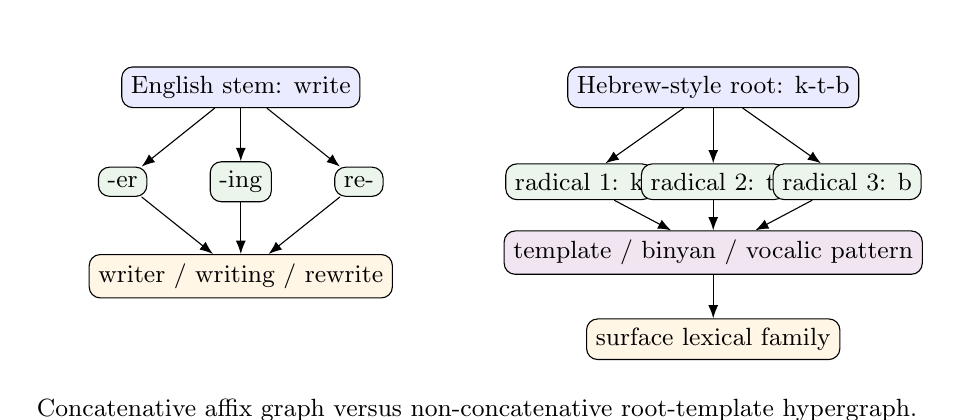
\begin{tikzpicture}[every node/.style={font=\small}, >=Latex]
\node[draw, rounded corners, fill=Blue!8] (engstem) at (-3,2) {English stem: write};
\node[draw, rounded corners, fill=Green!8] (engsuf1) at (-4.5,0.8) {-er};
\node[draw, rounded corners, fill=Green!8] (engsuf2) at (-3,0.8) {-ing};
\node[draw, rounded corners, fill=Green!8] (engsuf3) at (-1.5,0.8) {re-};
\node[draw, rounded corners, fill=Orange!10] (engword) at (-3,-0.4) {writer / writing / rewrite};
\draw[->] (engstem) -- (engsuf1);\draw[->] (engstem) -- (engsuf2);\draw[->] (engstem) -- (engsuf3);\draw[->] (engsuf1) -- (engword);\draw[->] (engsuf2) -- (engword);\draw[->] (engsuf3) -- (engword);
\node[draw, rounded corners, fill=Blue!8] (root) at (3,2) {Hebrew-style root: k-t-b};
\node[draw, rounded corners, fill=Green!8] (slot1) at (1.3,0.8) {radical 1: k};
\node[draw, rounded corners, fill=Green!8] (slot2) at (3,0.8) {radical 2: t};
\node[draw, rounded corners, fill=Green!8] (slot3) at (4.7,0.8) {radical 3: b};
\node[draw, rounded corners, fill=Purple!10] (templ) at (3,-0.1) {template / binyan / vocalic pattern};
\node[draw, rounded corners, fill=Orange!10] (surface) at (3,-1.2) {surface lexical family};
\draw[->] (root) -- (slot1);\draw[->] (root) -- (slot2);\draw[->] (root) -- (slot3);
\draw[->] (slot1) -- (templ);\draw[->] (slot2) -- (templ);\draw[->] (slot3) -- (templ);\draw[->] (templ) -- (surface);
\node at (0,-2.1) {Concatenative affix graph versus non-concatenative root-template hypergraph.};
\end{tikzpicture}
\caption{Original schematic comparing English-like concatenative morphology with Hebrew/Semitic root-template graph structure. Transliterations are used for compilation portability.}
\label{fig:hebrew_english}
\end{figure}

A TokenGT model can include both structures. For English, affix edges and subword edges may suffice for many tasks. For Hebrew, explicit root-template hyperedges can reduce the burden on subword tokenization and expose a linguistically meaningful graph. Recent work on Semitic Root Encoding and tokenization of Hebrew and Turkish supports the view that morphology-aware tokenization can matter, especially where standard subword segmentation obscures non-concatenative morphology \cite{Hatch2025,Samo2026}.

\section{Persistent topology for embedding and thought spaces}

\subsection{Why persistence is useful}

Embedding spaces are high-dimensional and unstable under rotations, basis changes, and training variation. A single nearest-neighbor list can be misleading. Persistent topology asks a more robust question: what qualitative shape features persist over a range of scales? If a group of token embeddings forms a robust semantic cluster, it should appear as a connected component before merging with unrelated tokens. If two reasoning paths form an alternative cycle in a graph-of-thought state, that cycle may appear as an $H_1$ feature. If a family of latent states surrounds an excluded region of representation space, higher homology may appear.

Persistence is not semantic interpretation by itself. It is a measurement layer. It becomes useful when paired with linguistic labels, causal interventions, probing, layer comparison, and task outcomes.

\subsection{Filtrations from transformer data}

A transformer supplies several filtrations:

\begin{enumerate}
\item \textbf{Embedding-distance filtration.} Vertices are tokens or graph tokens; edges appear when $\|z_i-z_j\|\le r$.
\item \textbf{Attention filtration.} Edges appear when attention weight $A_{ij}\ge \alpha$, often using decreasing threshold $\alpha$ or increasing cost $1-A_{ij}$.
\item \textbf{Mutual-information or probing filtration.} Edges appear when a learned relation score exceeds a threshold.
\item \textbf{Layer filtration.} The index $\ell$ itself is a filtration direction: complexes evolve across layers.
\item \textbf{Loop-time filtration.} In latent reasoning, complexes evolve across recurrent thought steps $t$.
\item \textbf{Distogram confidence filtration.} Edge $(i,j)$ appears when $\mathbb{P}(d_{ij}\le r)\ge q$.
\end{enumerate}

For a TokenGT language graph, the vertex set can include both original language nodes and induced edge tokens. This means a syntactic relation itself becomes a point in embedding space. Persistent analysis can ask whether dependency-edge tokens cluster with their endpoints, whether coreference edges form long-range components, or whether morphological hyperedge tokens form stable families across languages.

\subsection{Stability theorem}

The value of persistent homology rests partly on stability: small perturbations of distances or functions produce small perturbations of persistence diagrams.

\begin{theorem}[Stability of sublevel-set persistence, informal standard form]
Let $f,g:X\to\R$ be tame functions on a triangulable space $X$. Let $Dgm(f)$ and $Dgm(g)$ be their persistence diagrams for sublevel-set filtrations. Then the bottleneck distance satisfies
\[
d_B(Dgm(f),Dgm(g))\le \|f-g\|_\infty.
\]
\end{theorem}
\begin{proof}[Proof sketch]
If $\|f-g\|_\infty\le\eps$, then every sublevel set $X_f(a)=\{x:f(x)\le a\}$ is contained in $X_g(a+\eps)$, and $X_g(a)$ is contained in $X_f(a+\eps)$. These inclusions define an $\eps$-interleaving of the persistence modules. The algebraic stability theorem states that an $\eps$-interleaving implies bottleneck distance at most $\eps$.
\end{proof}

For language models, the theorem says that if distance functions or filtration scores change only slightly, persistence diagrams change only slightly. It does not say the chosen metric is meaningful. Metric choice remains the critical modeling decision.

\subsection{Persistent Laplacians}

Persistent homology captures topological invariants. Persistent Laplacians add spectral information. For a simplicial complex, the $p$-Hodge Laplacian is
\[
\Delta_p=\partial_{p+1}\partial_{p+1}^\top+\partial_p^\top\partial_p.
\]
Its kernel dimension equals $\beta_p$. Nonzero eigenvalues contain additional geometric information about cycles, cavities, and connectivity. Persistent topological Laplacians extend this across filtrations and have been proposed as richer descriptors for complex data \cite{WeiPersistentLaplacian2023}.

In a TokenGT language model, persistent Laplacian spectra could be used to measure:
\begin{enumerate}
\item whether a layer collapses too many syntactic components prematurely;
\item whether latent thought loops converge to stable low-dimensional manifolds;
\item whether cross-lingual morphology preserves root-template topology;
\item whether graph-of-thought exploration creates redundant cycles or useful alternative paths;
\item whether attention heads produce topological signatures associated with correct reasoning.
\end{enumerate}

\subsection{Topological regularization}

One can add topological objectives to training or finetuning. Let $\mathcal{D}_\ell(x)$ be a persistence diagram from layer $\ell$ for input $x$. A regularizer might encourage diagrams to match a target linguistic diagram $\mathcal{D}^{target}(x)$:
\[
\mathcal{L}_{topo}=\sum_{\ell\in\Lambda} d_B(\mathcal{D}_\ell(x),\mathcal{D}^{target}(x))^2.
\]
Alternatively, it can penalize topological collapse:
\[
\mathcal{L}_{collapse}=\sum_\ell \max(0,\delta-P_{H_0}(\mathcal{D}_\ell)),
\]
where $P_{H_0}$ is total persistence in dimension $0$. Differentiable persistence methods exist, but they add computational cost and can be unstable if used naively. For near-term research, topology may be more reliable as an analysis and model-selection tool than as a training objective.

\subsection{Persistence and human memory}

Persistent topology also offers a metaphor and analysis tool for biological memory. Neural population activity during tasks often lies on low-dimensional manifolds. Learning can alter manifold geometry. Engram ensembles can be viewed as persistent components in activity space or connectivity space across perturbations. Gap-junction and astrocyte networks can be analyzed as weighted graphs whose Laplacian spectra affect synchronization. But direct application to human learning requires neural data: calcium imaging, electrophysiology, connectomics, fMRI manifolds, or single-cell omics. The transformer setting is easier because all hidden states are observable.

\section{Tropical geometry of neural networks and attention}

\subsection{ReLU networks as polyhedral maps}

A ReLU network is piecewise affine. Each ReLU unit partitions its input by a hyperplane; a layer composes such partitions; a deep network creates a polyhedral complex of linear regions. Tropical geometry gives a language for max-plus piecewise-linear functions. Zhang, Naitzat, and Lim showed that ReLU networks are closely related to tropical rational maps, and that depth can exponentially increase expressivity through polyhedral subdivision \cite{ZhangTropical2018}. Subsequent work refines this picture using real tropical geometry and activation polytopes \cite{Brandenburg2024}.

For a transformer, the MLP sublayers are often GELU rather than ReLU, so the exact tropical representation is approximate unless one uses piecewise-linear approximations. Attention is smooth because of softmax, but its low-temperature or high-confidence limit is tropical-like: max selection replaces averaging.

\subsection{Zero-temperature attention}

Let scores $s_i=q^\top k_i/\sqrt d$. The attention output at temperature $\tau$ is
\[
y_\tau=\sum_i \frac{e^{s_i/\tau}}{\sum_j e^{s_j/\tau}}v_i.
\]

\begin{proposition}[Hard-selection limit of attention]
If $m=\argmax_i s_i$ is unique, then $\lim_{\tau\to0^+}y_\tau=v_m$.
\end{proposition}
\begin{proof}
For $i\ne m$, $s_i-s_m<0$, so $e^{(s_i-s_m)/\tau}\to0$. Dividing numerator and denominator by $e^{s_m/\tau}$ gives attention weight on $m$ tending to $1$ and all others tending to $0$.
\end{proof}

If multiple scores tie, the limit is a convex average over maximizers. This matters for reasoning. Many discrete algorithms, such as shortest paths and dynamic programming, use min-plus or max-plus recurrences. Softmax attention can approximate a softened version; tropical attention mechanisms explicitly operate in the max-plus semiring and have been proposed for neural algorithmic reasoning \cite{HashemiTropicalAttention2025}. Very recent work also attempts a tropical geometry framework for transformer expressivity and spatial partitioning \cite{TransformerTropical2026}. These results are promising but newer than the core transformer literature and should be treated as developing.

\subsection{Tropical cells and persistent features}

Tropical geometry and persistence are complementary. Tropical analysis describes the polyhedral cells induced by neural maps. Persistence describes topological features of point clouds or functions across scales. In a transformer layer, a set of input embeddings may be mapped through a sequence of smooth and piecewise-linear transformations. If attention is high-confidence, the map behaves like a selection over polyhedral regions. If MLPs are piecewise-linear approximated, the whole block partitions input space into cells.

One can therefore analyze a latent reasoning trajectory $z_0,z_1,\ldots,z_T$ in two ways:
\begin{enumerate}
\item \textbf{Tropical path:} which max-affine regions or attention argmax cells does the trajectory traverse?
\item \textbf{Persistent path:} what topological features appear in the point cloud of token/thought states along the trajectory?
\end{enumerate}
A stable reasoning process may correspond to a trajectory that enters a small set of polyhedral cells while maintaining a persistent graph structure corresponding to the problem's relational structure. A brittle process may jump between cells, collapse topology, or create spurious loops.

\begin{figure}[H]
\centering
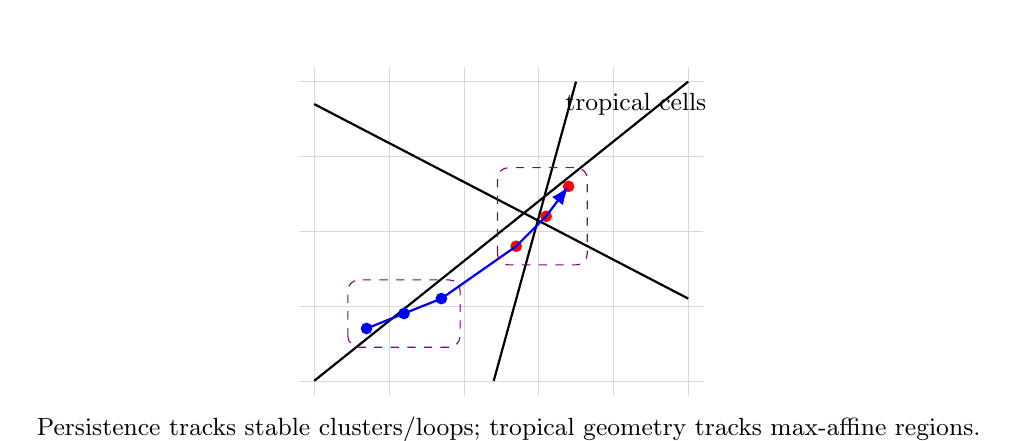
\begin{tikzpicture}[scale=0.95, every node/.style={font=\small}, >=Latex]
\draw[step=1.0, gray!30, very thin] (-0.2,-0.2) grid (5.2,4.2);
\draw[thick] (0,0) -- (5,4);
\draw[thick] (0,3.7) -- (5,1.1);
\draw[thick] (2.4,0) -- (3.5,4);
\node at (4.3,3.7) {tropical cells};
\filldraw[Blue] (0.7,0.7) circle (2pt);
\filldraw[Blue] (1.2,0.9) circle (2pt);
\filldraw[Blue] (1.7,1.1) circle (2pt);
\filldraw[Red] (2.7,1.8) circle (2pt);
\filldraw[Red] (3.1,2.2) circle (2pt);
\filldraw[Red] (3.4,2.6) circle (2pt);
\draw[->, thick, Blue] (0.7,0.7) -- (1.2,0.9) -- (1.7,1.1) -- (2.7,1.8) -- (3.1,2.2) -- (3.4,2.6);
\draw[rounded corners, dashed, Purple] (0.45,0.45) rectangle (1.95,1.35);
\draw[rounded corners, dashed, Purple] (2.45,1.55) rectangle (3.65,2.85);
\node[align=center] at (2.6,-0.65) {Persistence tracks stable clusters/loops; tropical geometry tracks max-affine regions.};
\end{tikzpicture}
\caption{Original schematic of the persistence-tropical interface. A latent trajectory crosses polyhedral regions while its point-cloud topology can be measured across scales.}
\label{fig:tropical_persistence}
\end{figure}

\subsection{The tropical view of parsing}

Parsing often involves max-scoring structures: maximum spanning tree for dependency parsing, CKY dynamic programming for context-free parsing, Viterbi decoding for hidden Markov models, and shortest-path computations for some graph algorithms. These are naturally max-plus or min-plus computations. A transformer with tropical attention or high-confidence attention may implement approximations to such combinatorial selection. TokenGT language graphs make the candidate parse edges explicit; tropical reasoning can select among them; persistence can test whether the selected structure is geometrically robust.

This suggests a hybrid objective: train a TokenGT model to produce parse or reasoning graphs whose scores are compatible with a tropical dynamic program while simultaneously preserving topological stability of embedding clusters. Such a model would be more interpretable than a pure sequence model because its intermediate objects are graph edges, simplexes, and trajectories.

\section{Latent reasoning loops as dynamical systems}

\subsection{Deterministic loops}

Consider a looped latent transformer
\[
z_{t+1}=F_\theta(z_t,x),\qquad t=0,\ldots,T-1.
\]
If $F_\theta$ is a contraction in $z$, then the loop converges to a unique fixed point. If not, it may cycle, diverge, or exhibit multiple attractors. Layer normalization and residual connections complicate the analysis. Empirical work on looped transformers suggests that they can emulate iterative algorithms and sometimes converge to stable fixed-point behavior beyond the number of loop iterations seen in training \cite{YangLooped2024,Saunshi2025}.

\begin{theorem}[Contraction fixed-point theorem for latent loops]
Let $(\calX,d)$ be a complete metric space and $F_x:\calX\to\calX$ satisfy
\[
d(F_x(z),F_x(z'))\le c d(z,z')
\]
for all $z,z'$ and some $0<c<1$. Then there is a unique fixed point $z^*(x)$ and $z_t\to z^*(x)$ for every initial state.
\end{theorem}
\begin{proof}
This is Banach's fixed-point theorem. The iterates form a Cauchy sequence because $d(z_{t+1},z_t)\le c^t d(z_1,z_0)$. Completeness gives a limit $z^*$. Continuity of $F_x$ gives $F_x(z^*)=z^*$. If $u$ and $v$ are fixed points, $d(u,v)=d(F_x(u),F_x(v))\le c d(u,v)$, so $d(u,v)=0$.
\end{proof}

A contraction is desirable for stable inference but may be too restrictive for search. Reasoning often requires maintaining alternatives rather than collapsing immediately. Coconut's reported breadth-first-like latent behavior is interesting precisely because a continuous state may encode multiple alternatives before committing \cite{Hao2024}.

\subsection{Stochastic loops and ergodicity}

Let a latent reasoning loop be stochastic:
\[
z_{t+1}\sim P_\theta(\cdot\mid z_t,x).
\]
This may represent sampling soft thought perturbations, choosing graph expansions, retrieving external documents, or applying tools. Under strong mixing assumptions, the loop has an invariant distribution.

\begin{theorem}[Doeblin ergodicity for a stochastic reasoning loop]
Let $P$ be a Markov kernel on a measurable state space. Suppose there exist $\eps>0$ and a probability measure $\nu$ such that
\[
P(z,A)\ge \eps\nu(A)
\]
for all states $z$ and measurable sets $A$. Then $P$ has a unique invariant distribution $\pi$, and
\[
\|\mu P^t-\pi\|_{TV}\le (1-\eps)^t
\]
for every initial distribution $\mu$.
\end{theorem}
\begin{proof}
The minorization condition implies that each transition can be decomposed as $P=\eps \nu +(1-\eps)Q_z$ for a residual kernel $Q$. Coupling two chains by using the common $\nu$ refresh event makes them meet with probability at least $\eps$ each step. The probability of not coupling by time $t$ is at most $(1-\eps)^t$, which bounds total variation distance and implies uniqueness.
\end{proof}

This theorem is too strong for most real LLM loops, but it clarifies what is missing. To claim ergodicity, one needs explicit stochastic exploration and enough smoothing or refresh to avoid absorbing bad states. A GFlowNet objective supplies a different guarantee: terminal samples proportional to reward if flow constraints are satisfied.

\subsection{Reasoning trajectories as graph-valued paths}

A graph-of-thought latent state can be written
\[
S_t=(G_t,Z_t,C_t),
\]
where $G_t$ is a typed thought graph, $Z_t$ assigns embeddings to its nodes and edges, and $C_t$ is controller state. An action can add a node, add an edge, merge nodes, refine a node, call a tool, verify a subclaim, or emit an answer. The transition is
\[
S_{t+1}=\mathcal{T}_\theta(S_t,a_t,\xi_t),
\]
where $\xi_t$ is stochasticity. The reward can be terminal or process-based:
\[
R(S_T)=R_{answer}R_{proof}R_{consistency}R_{cost}^{-1}.
\]
A continuous GFlowNet can sample such trajectories if the state space is formulated with suitable densities and backward kernels.

\begin{figure}[H]
\centering
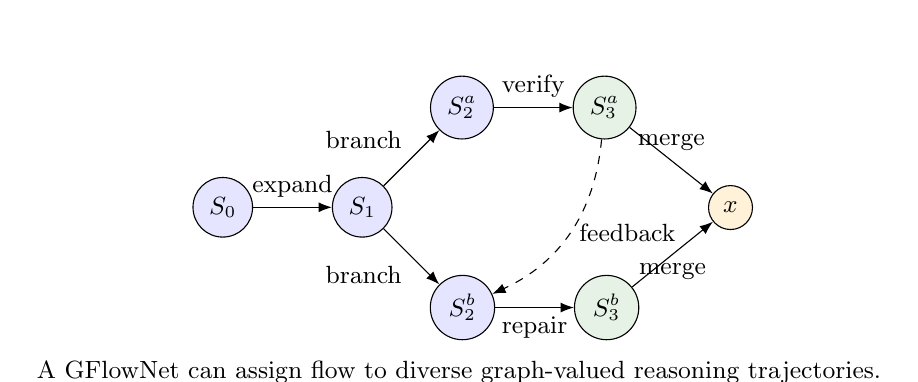
\begin{tikzpicture}[every node/.style={font=\small}, >=Latex, node distance=1cm]
\node[draw, circle, fill=Blue!10] (s0) {$S_0$};
\node[draw, circle, fill=Blue!10, right=of s0] (s1) {$S_1$};
\node[draw, circle, fill=Blue!10, above right=of s1] (s2a) {$S_2^a$};
\node[draw, circle, fill=Blue!10, below right=of s1] (s2b) {$S_2^b$};
\node[draw, circle, fill=Green!10, right=of s2a] (s3a) {$S_3^a$};
\node[draw, circle, fill=Green!10, right=of s2b] (s3b) {$S_3^b$};
\node[draw, circle, fill=Orange!15, right=1.3cm of $(s3a)!0.5!(s3b)$] (x) {$x$};
\draw[->] (s0) -- node[above] {expand} (s1);
\draw[->] (s1) -- node[above left] {branch} (s2a);
\draw[->] (s1) -- node[below left] {branch} (s2b);
\draw[->] (s2a) -- node[above] {verify} (s3a);
\draw[->] (s2b) -- node[below] {repair} (s3b);
\draw[->] (s3a) -- node[above] {merge} (x);
\draw[->] (s3b) -- node[below] {merge} (x);
\draw[->, dashed, bend left] (s3a) to node[right] {feedback} (s2b);
\node[align=center] at (3,-2.1) {A GFlowNet can assign flow to diverse graph-valued reasoning trajectories.};
\end{tikzpicture}
\caption{Original schematic of a graph-valued latent reasoning state space. Terminal answers can be sampled in proportion to verifier reward rather than greedily selected.}
\label{fig:gflownet_got}
\end{figure}

\subsection{Inference-time scaling}

Inference-time scaling uses more computation at test time to improve answers. Methods include self-consistency, best-of-$N$, tree search, graph-of-thought reasoning, verifier-guided search, process reward models, debate, reflection, and latent loops. Recent surveys emphasize that test-time scaling requires decisions about what to scale, how to allocate compute, where to use verifiers, and how to evaluate cost-quality tradeoffs \cite{ZhangTTSSurvey2025,Balachandran2025,LiSearch2025}. Latent reasoning adds another dimension: scale hidden-state computation rather than visible tokens.

The biological analogy is deliberation and recurrent processing. A human can spend more time thinking, simulate alternatives, retrieve memories, and revise hypotheses. But human deliberation is constrained by attention, working memory, emotion, fatigue, and metacognition. LLM test-time scaling is constrained by token budget, latency, verifier quality, sampling diversity, and context length.

\section{Toward TokenGT latent graph reasoning with topology and tropical structure}

\subsection{Proposed architecture}

The proposed architecture, called here \emph{TopoTropical TokenGT Latent Reasoner} (TT-TokGT-LR), has six modules.

\begin{enumerate}
\item \textbf{Graph constructor.} Build a typed language graph from text using tokenization, dependency parsing, semantic roles, coreference, discourse, and morphology. For Hebrew and other Semitic languages, add root-template hyperedges when available.
\item \textbf{TokenGT encoder.} Convert nodes, edges, and hyperedges into a sequence of tokens with type, incidence, position, and optional orthogonal identifiers.
\item \textbf{Transformer backbone.} Apply standard self-attention and MLP blocks. The model can be initialized from a language model when dimensions and token interfaces permit.
\item \textbf{Latent loop.} Feed selected hidden states or learned soft thought tokens back into the graph-token sequence for $T$ reasoning steps.
\item \textbf{Topological monitor.} Compute distograms, persistence diagrams, persistent Laplacian spectra, and layer/loop topology summaries.
\item \textbf{Tropical/verifier controller.} Use max-plus-inspired scoring, verifiers, and optional GFlowNet flow matching to select or sample graph-of-thought trajectories.
\end{enumerate}

\begin{figure}[H]
\centering
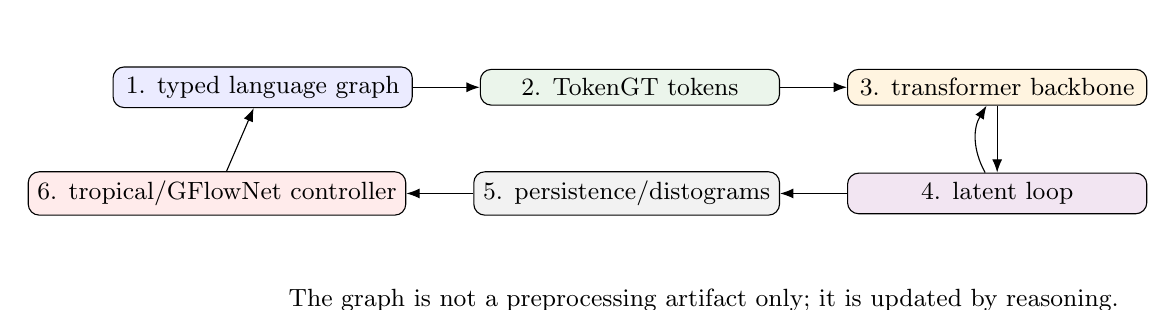
\begin{tikzpicture}[every node/.style={font=\small}, >=Latex, node distance=0.85cm]
\node[draw, rounded corners, fill=Blue!8, minimum width=3.8cm] (g) {1. typed language graph};
\node[draw, rounded corners, fill=Green!8, right=of g, minimum width=3.8cm] (tg) {2. TokenGT tokens};
\node[draw, rounded corners, fill=Orange!12, right=of tg, minimum width=3.8cm] (tr) {3. transformer backbone};
\node[draw, rounded corners, fill=Purple!10, below=of tr, minimum width=3.8cm] (loop) {4. latent loop};
\node[draw, rounded corners, fill=gray!10, left=of loop, minimum width=3.8cm] (topo) {5. persistence/distograms};
\node[draw, rounded corners, fill=Red!8, left=of topo, minimum width=3.8cm] (ctrl) {6. tropical/GFlowNet controller};
\draw[->] (g) -- (tg);
\draw[->] (tg) -- (tr);
\draw[->] (tr) -- (loop);
\draw[->] (loop) -- (topo);
\draw[->] (topo) -- (ctrl);
\draw[->] (ctrl) -- (g);
\draw[->, bend left] (loop) to (tr);
\node[align=center] at (5.6,-2.7) {The graph is not a preprocessing artifact only; it is updated by reasoning.};
\end{tikzpicture}
\caption{Original architecture schematic for TT-TokGT-LR. The language graph, latent thought graph, topological monitor, and controller form an inference-time dynamical system.}
\label{fig:architecture}
\end{figure}

\subsection{Formal state representation}

Let the reasoning state be
\[
S_t=(G_t,X_t,H_t,\mathcal{P}_t,\mathcal{C}_t),
\]
where $G_t$ is a typed graph, $X_t$ are graph-token features, $H_t$ are hidden states, $\mathcal{P}_t$ are topological summaries, and $\mathcal{C}_t$ is controller memory. A transition consists of:
\[
\begin{aligned}
X_t &= \Phi(G_t),\\
H_t &= T_\theta(X_t,Z_t),\\
Z_{t+1} &= L_\theta(H_t,Z_t),\\
\mathcal{P}_t &= \operatorname{Persist}(H_t,G_t),\\
a_t &\sim \pi_\phi(\cdot\mid H_t,\mathcal{P}_t,\mathcal{C}_t),\\
G_{t+1} &= U(G_t,a_t).
\end{aligned}
\]
Here $Z_t$ are continuous thought tokens, $L_\theta$ is a latent update, and $U$ changes the thought graph. The controller can be trained by reinforcement learning, supervised traces, process reward models, or GFlowNet objectives.

\subsection{Losses}

A composite training or finetuning objective might be
\[
\mathcal{L}=\mathcal{L}_{LM}+\lambda_{task}\mathcal{L}_{task}+\lambda_{graph}\mathcal{L}_{graph}+\lambda_{topo}\mathcal{L}_{topo}+\lambda_{flow}\mathcal{L}_{GFlow}+\lambda_{cost}\mathcal{L}_{cost}.
\]
The components can be:

\begin{align*}
\mathcal{L}_{LM} &= -\sum_t \log p_\theta(x_{t+1}\mid x_{\le t},G_t),\\
\mathcal{L}_{graph} &= \text{edge/type prediction loss for syntax, morphology, semantics},\\
\mathcal{L}_{topo} &= \sum_{\ell,t} d(\mathcal{D}_{\ell,t},\mathcal{D}^{target}_{t})^2,\\
\mathcal{L}_{GFlow} &= \E_\tau\left[\left(\log Z+\sum_t\log P_F-\log R(x)-\sum_t\log P_B\right)^2\right],\\
\mathcal{L}_{cost} &= \E[T+|G_T|+\text{tool calls}].
\end{align*}

A conservative research plan would first use topology as monitoring rather than as a direct loss. Direct topological loss can be introduced only after verifying that the diagrams correlate with task success and linguistic structure.

\subsection{Algorithm sketch}

\begin{lstlisting}
Input: text/document x, optional language tag, budget B
G0 = build_language_graph(x)
if language is Semitic:
    add_root_template_hyperedges(G0)
Z0 = initialize_soft_thought_tokens(G0)
S0 = (G0, Z0)
for t in 0..B-1:
    Xt = TokenGT_encode(Gt, Zt)
    Ht = Transformer(Xt)
    Dt = embedding_distogram(Ht)
    Pt = persistent_summaries(Dt, Gt)
    scores = tropical_or_verifier_scores(Ht, Pt, Gt)
    action = controller_sample_or_select(scores)
    Gt+1, Zt+1 = update_graph_and_latents(Gt, Zt, action, Ht)
return decode_answer(G_B, Z_B, H_B)
\end{lstlisting}

This algorithm treats reasoning as graph-state evolution. It differs from ordinary chain-of-thought by allowing non-linear thought topology, hidden continuous thoughts, morphology-aware graph tokens, and topological monitoring.

\subsection{Evaluation}

Evaluation should not rely only on final answer accuracy. A rigorous program should measure:
\begin{enumerate}
\item final task accuracy on reasoning, parsing, morphology, translation, and cross-lingual tasks;
\item calibration and uncertainty under perturbation;
\item topology-task correlation: do persistent features predict correct reasoning?
\item graph faithfulness: do thought edges correspond to actual dependencies used by the model?
\item ablations: remove morphology edges, remove persistence monitor, remove latent loop, remove GFlowNet sampling;
\item efficiency: answer quality per token, FLOP, and wall-clock cost;
\item interpretability: whether topological and tropical summaries explain failure modes;
\item multilingual robustness, especially between concatenative and non-concatenative morphology.
\end{enumerate}

\subsection{Potential failure modes}

The architecture can fail in predictable ways. The graph constructor may add wrong edges; the model may overfit parser artifacts; topological regularization may preserve the wrong clusters; latent loops may collapse to fixed points too early or drift chaotically; GFlowNet rewards may be misspecified; tropical hard selection may harm tasks requiring uncertainty; morphology-aware tokenization may improve rare forms while hurting high-resource common forms; cross-lingual root extraction may inject linguistic assumptions that are debated among morphologists.

A particularly important failure mode is \emph{topological pareidolia}: finding persistent features and assigning semantic meaning after the fact. The remedy is pre-registered hypotheses, controls with randomized labels, perturbation tests, and causal interventions on graph edges or attention heads.

\section{Biological analogues of the proposed architecture}

The architecture above is not a brain model, but it resonates with several biological motifs.

First, graph-tokenization resembles the fact that the brain does not process language as a flat string only. Auditory, orthographic, phonological, morphological, syntactic, semantic, and pragmatic representations interact through a network. Second, latent loops resemble recurrent cortical and hippocampal processing. Third, GFlowNet-like diverse trajectory sampling resembles maintaining multiple hypotheses rather than greedy decoding. Fourth, persistent topology resembles the robustness of neural population manifolds and engram overlap. Fifth, tropical max-plus operations resemble hard selection and winner-take-all computations in inhibitory circuits, though biological winner-take-all is implemented by spiking networks and inhibition rather than algebraic max.

The sharpest difference remains learning. In the proposed architecture, the main learning still occurs by gradient descent unless one adds online memory writing. In humans, every deliberation can modify future learning through synaptic, neuromodulatory, and systems-level plasticity. An agentic transformer can mimic this only by explicitly writing to external memory or updating parameters/adapters.

\section{Detailed biochemistry-to-transformer comparison}

\subsection{Calcium and gradients}

Calcium is a local biochemical signal. It enters through NMDA receptors, voltage-gated calcium channels, and other routes, and it can trigger kinases, phosphatases, transcriptional pathways, and structural changes. It is not a loss gradient. A gradient is a derivative of an objective with respect to a parameter. The analogy is that both are credit-related signals that regulate change. The difference is that calcium is local, nonlinear, thresholded, buffered, spatially compartmentalized, and tied to physical chemistry.

\begin{longtable}{p{0.25\linewidth}p{0.32\linewidth}p{0.32\linewidth}}
\toprule
Biochemical signal & Computational role & Transformer analogue \\
\midrule
Ca$^{2+}$ influx & Coincidence detection, kinase/phosphatase activation, plasticity threshold & Local activation statistics or eligibility trace, not gradient \\
CaMKII & Synaptic plasticity organizer, phosphorylation, structural binding & Learned update module or persistent local state; weak analogue \\
CREB transcription & Long-term consolidation and protein synthesis & Durable parameter/memory write; no direct standard analogue \\
BDNF/TrkB & Growth, survival, synaptic modulation & Learning-rate or plasticity support signal; weak analogue \\
Dopamine & Reward prediction, salience, plasticity gating & Reinforcement signal/reward model, but biology is richer \\
Astrocyte lactate/metabolism & Energy support, modulation of plasticity & Compute/memory resource support; very weak analogy \\
Gap-junction conductance & Electrical/metabolic coupling & Graph Laplacian/residual coupling; mathematical analogue only \\
\bottomrule
\caption{Biochemical mechanisms and careful transformer analogues.}
\end{longtable}

\subsection{Synaptic consolidation and model finetuning}

Late LTP requires protein synthesis and gene expression in many settings. Systems consolidation redistributes memory dependence across hippocampal and cortical networks. In transformers, finetuning or continued pretraining changes weights persistently; retrieval-augmented memory writes store new text externally; LoRA adapters store task-specific deltas. These are closer to consolidation than in-context learning is. However, biological consolidation is not simply additional gradient steps. It involves replay, sleep, neuromodulation, synaptic tagging and capture, dendritic localization, and homeostatic constraints.

\subsection{Homeostasis and normalization}

Neural systems have homeostatic plasticity: synaptic scaling, intrinsic excitability adjustment, inhibitory balance, and metaplasticity. Transformers have layer normalization, RMS normalization, residual scaling, weight decay, optimizer adaptivity, gradient clipping, and sometimes activation regularization. Both maintain activity within useful ranges. But biological homeostasis is an active cellular process over minutes to days; layer normalization is a deterministic algebraic operation.

\subsection{Metaplasticity and optimizer state}

Metaplasticity means the plasticity of plasticity: prior activity changes the threshold or rule for future plasticity. In machine learning, optimizer state such as Adam moments changes future parameter updates. This is one of the better analogies. Adam maintains first and second moment estimates,
\[
m_t=\beta_1m_{t-1}+(1-\beta_1)g_t,
\quad
v_t=\beta_2v_{t-1}+(1-\beta_2)g_t^2,
\]
and updates parameters with normalized moments. Metaplasticity changes synaptic update thresholds through biochemical state. Both are history-dependent update modulators. Yet Adam is global and algorithmic; metaplasticity is local and biochemical.

\section{Memory, retrieval, and weights in both systems}

\subsection{What is a weight?}

A useful abstraction writes a system's output as
\[
y=F(x;\Theta,S),
\]
where $\Theta$ are persistent parameters and $S$ is temporary state. In a transformer, $\Theta$ is clear: tensors. In a brain, $\Theta$ is not sharply separable from $S$ because many biochemical states are persistent on intermediate timescales. A spine's receptor composition may last minutes to days; gene expression may last hours; structural changes may last longer; neuromodulatory state may last seconds to minutes. Thus brain ``weights'' are temporally stratified.

\begin{definition}[Temporally stratified parameter]
A variable $\theta_i$ is a temporally stratified parameter if its relaxation time $\tau_i$ is long compared with computation time but not necessarily long compared with learning or consolidation time. Biological learning contains many such variables. Standard transformer inference usually has a single persistent parameter class and temporary activations, unless external memory or online adaptation is added.
\end{definition}

\subsection{Associative retrieval as kernel regression}

Attention can be viewed as kernel regression:
\[
y(q)=\sum_i \frac{\kappa(q,k_i)}{\sum_j\kappa(q,k_j)}v_i,
\quad \kappa(q,k)=\exp(q^\top k/\sqrt d).
\]
Hippocampal retrieval can also be abstracted as kernel-like pattern completion: cues similar to stored patterns activate associated content. The difference is that biological similarity is learned through recurrent circuitry and plastic synapses, not a single dot product in a learned embedding space.

\subsection{Memory editing and reconsolidation}

Biological retrieval can open a reconsolidation window during which a memory can be modified. Transformer retrieval does not modify stored parameters unless the system has explicit online learning. However, an agent with memory writing can mimic reconsolidation: retrieving a memory, updating it with new evidence, and writing back. This is not inherent in transformers; it is a system design choice.

\subsection{Forgetting}

Biological forgetting can result from synaptic weakening, engram inhibition, systems reorganization, interference, neurogenesis, retrieval failure, or active molecular processes. Transformer forgetting occurs during training as catastrophic forgetting, during context as truncation, in retrieval systems as deletion or indexing failure, and in generation as failure to activate stored knowledge. Continual learning tries to mitigate catastrophic forgetting with replay, regularization, adapters, memory, and modularity. The biological analogy to replay is strong at the algorithmic level, particularly for hippocampal-cortical consolidation, but the mechanisms differ.

\section{Mathematical bridges and non-bridges}

\subsection{Graph Laplacians}

Graph Laplacians appear in gap-junction coupling, diffusion maps, graph neural networks, spectral clustering, and persistent Laplacians. This is a genuine mathematical bridge. If $L$ is a graph Laplacian, then $\dot x=-Lx$ smooths $x$ over the graph. Gap junctions smooth voltage. Graph neural layers often smooth features. Attention can create a data-dependent random-walk matrix. Persistent Laplacians study spectra across topological scales.

But a graph Laplacian by itself has no semantics. The graph edges and state variables determine meaning. A gap-junction graph over interneurons is not a dependency parse graph; a dependency parse graph is not an attention graph; an attention graph is not a connectome.

\subsection{Energy functions}

Energy functions appear in Hopfield networks, Boltzmann machines, predictive coding, variational inference, and some models of neural dynamics. Transformer decoding is not usually energy minimization, but attention has an energy-like log-sum-exp form and modern Hopfield theory gives a direct energy interpretation. Latent loops may have implicit Lyapunov functions if trained to converge. Biological circuits may minimize or sample from energy-like objectives under some models, but the brain is not globally minimizing a known scalar loss.

\subsection{Persistence and engrams}

A persistent homology class is a topological feature that survives across scales. An engram is a physical memory trace. The analogy is tempting: persistent topological features in neural state space may correspond to stable memory structure. But a persistence bar is not an engram. It is a statistic. To link it to engrams, one needs causal evidence that manipulating the corresponding cells or states affects recall.

\subsection{Tropical selection and biological winner-take-all}

The tropical max operation resembles winner-take-all selection. Biological circuits can implement winner-take-all behavior through inhibition, recurrent excitation, and spiking thresholds. Transformers can implement hard selection through low-temperature attention or argmax decoding. The common abstraction is max selection; the mechanisms differ.

\section{Original synthesis: a graph-topological theory of latent language reasoning}

\subsection{Core hypothesis}

The central hypothesis is:

\begin{quote}
A language reasoning model generalizes better when its latent computation preserves the stable multiscale topology of the task's relational graph while allowing tropical-like discrete selection over candidate reasoning structures.
\end{quote}

In simpler terms, the model should keep the right graph shape while making sharp decisions when necessary. Persistence measures ``keeping the right shape.'' Tropical geometry measures ``making sharp piecewise-linear selections.'' TokenGT supplies the graph substrate. Latent loops supply iterative computation. GFlowNets supply diverse trajectory sampling.

\subsection{Formal version}

Let $G_x$ be a task graph for input $x$, and let $Y_x$ be a target output. Let $\mathcal{T}(G_x)$ be a topological signature of the graph, such as persistent diagrams of a graph metric or clique complex. Let $H_t$ be model hidden states and $\mathcal{T}(H_t)$ their embedding topology. Let $C_t$ be a tropical cell assignment induced by high-confidence attention/MLP regions. The hypothesis can be formalized as:
\[
\Pr(\hat Y=Y\mid x) \text{ increases when } d(\mathcal{T}(H_t),\mathcal{T}(G_x)) \text{ is small and } C_t \text{ stabilizes before decoding.}
\]
This is testable. One can compute topological distances and cell-transition statistics and regress task success against them, with controls for model size and confidence.

\subsection{Predictions}

The theory predicts:
\begin{enumerate}
\item Correct multi-hop reasoning will show persistent connected components corresponding to entities and relations before final answer generation.
\item Incorrect reasoning will often show topological collapse, spurious cycles, or unstable cell transitions.
\item TokenGT graph inputs will improve tasks where relational structure is sparse but crucial, especially long-range dependencies and non-concatenative morphology.
\item Hebrew root-template tasks will benefit from explicit root/template hyperedges more than English affix tasks benefit from explicit affix edges, because ordinary subword tokenization already captures many English concatenative cues.
\item GFlowNet-guided graph-of-thought sampling will improve diversity and calibration when multiple valid reasoning paths exist.
\item Tropical attention or low-temperature heads will help algorithmic parsing and dynamic-programming-like tasks but may hurt ambiguity-sensitive semantic tasks unless combined with uncertainty-preserving soft heads.
\end{enumerate}

\subsection{Experimental design}

A rigorous experiment would include:
\begin{enumerate}
\item Benchmarks: dependency parsing, semantic role labeling, multi-hop QA, theorem/proof tasks, Hebrew morphological analogy, Arabic/Hebrew translation, synthetic graph reasoning, and long-context coreference.
\item Models: baseline decoder-only transformer, graph-augmented transformer, TokenGT encoder-decoder, TokenGT with latent loops, TokenGT with topology monitoring, TokenGT with GFlowNet controller.
\item Ablations: remove syntax edges, remove morphology edges, randomize edges, replace distograms with deterministic distances, remove loop recurrence, remove verifier.
\item Metrics: accuracy, exact match, F1, calibration, compute cost, topological distances, graph faithfulness, trajectory diversity, robustness to paraphrase and word-order perturbation.
\item Statistical tests: bootstrap confidence intervals, paired tests, multiple-comparison correction, and held-out languages/domains.
\end{enumerate}

\section{Limits of the analogy to human learning}

The proposed framework can be biologically inspired, but it is not a theory of the human brain. Several limits are decisive.

First, biological learning is online and lifelong; transformer training is usually offline and batch-based. Second, biological learning is local and physically constrained; transformer learning uses exact automatic differentiation through a global computational graph. Third, biological neurons spike and release chemicals; transformer units compute dense linear algebra. Fourth, gap junctions are conductance channels; attention is not an electrical synapse. Fifth, human memory includes embodiment, affect, sleep, social context, and action; language models usually operate on text and tool outputs. Sixth, biological systems have intrinsic goals and homeostatic needs; transformer objectives are externally specified.

These differences are not defects in transformers; they are category distinctions. The value of comparison is to sharpen architecture and analysis, not to erase biology.

\section{Implications for interpretability and safety}

Graph-token latent reasoning with topological monitoring could improve interpretability. Instead of inspecting only generated chain-of-thought, one can inspect thought graphs, topology summaries, verifier scores, and latent loop convergence. This is useful because natural-language chain-of-thought may be incomplete or unfaithful to internal computation. If reasoning is latent-state trajectory formation, then interpretability should analyze trajectories, not only decoded rationales.

However, latent reasoning also creates risks: hidden thoughts are less directly auditable; graph controllers can optimize reward models in unintended ways; topological metrics can be gamed; external memory writes can preserve erroneous information. Safety requires independent verifiers, causal faithfulness tests, constrained memory writes, and robust monitoring.


\section{Engineering a sub-15B TokenGT reasoning agent}
\label{sec:engineering-agent}

The preceding sections describe a mathematical view: language is not merely a sequence, but a typed relational object whose stable structure can be represented by graphs, monitored by persistence, and sharpened by tropical selection. This section converts that view into a concrete model-building program. The target is not a frontier-scale general model. The target is a small, high-quality reasoning agent: a model below roughly $15$ billion parameters, preferably much smaller for from-scratch training, with an effective long-context interface, robust tool use, Lean proof checking, mathematical reasoning, code execution, sequence-backed biochemical reasoning, and UMA-oracle-conditioned candidate evaluation.

The hardware assumption is deliberately severe: a single consumer NVIDIA RTX 4090. Its $24$GB memory budget is valuable but small relative to modern pretraining needs \cite{Nvidia4090}. It can support careful experimentation, high-quality adapter training, synthetic-data pipelines, distillation, and small from-scratch models. It cannot support naive full-parameter training of a $15$B dense transformer at $256$K tokens with quadratic attention.

\begin{proposition}[Single-4090 feasibility envelope]
\label{prop:4090-envelope}
A single $24$GB GPU is not a plausible platform for full-parameter Adam training of a dense $15$B transformer, and it is not a plausible platform for dense full-attention training at $256$K tokens. It is, however, a plausible platform for: (i) from-scratch training of small models with short-to-medium contexts, (ii) QLoRA or LoRA adaptation of larger open models, (iii) continued pretraining of quantized or adapter-augmented models, (iv) verifier-guided synthetic-data generation and curation, and (v) retrieval- or graph-memory systems whose \emph{effective} context exceeds the raw training window.
\end{proposition}

\begin{proof}
Let $P$ be the number of trainable parameters. A simple mixed-precision Adam implementation stores at least fp16 or bf16 weights, gradients, optimizer first and second moments, and often fp32 master weights. A common lower-order estimate is
\[
M_{\rm Adam}\approx 2P+2P+4P+4P+4P=16P \quad \text{bytes},
\]
up to implementation details. Even a more optimistic accounting remains far above $24$GB for $P=15\times 10^9$. For attention, a dense attention matrix has $n^2$ pairwise scores per head. At $n=256{,}000$, $n^2\approx 6.55\times 10^{10}$ entries, so materializing attention is impossible and even exact streaming attention is compute-heavy. Flash-style kernels reduce memory traffic but not the underlying quadratic interaction count. Hence the only realistic single-4090 routes are small dense pretraining, parameter-efficient adaptation, sparse or block attention, retrieval, recurrence, and graph memory. \qedhere
\end{proof}

The useful design question is therefore not ``How can one train the largest possible model?'' but rather ``How can one force a small model to spend its limited capacity on durable structure?'' The answer proposed here is to encode structure explicitly and to verify reasoning whenever possible.

\begin{table}[H]
\centering
\small
\caption{Practical training tracks for a single RTX 4090. Parameter counts are envelopes, not guarantees; they depend on optimizer, quantization, sequence length, batch size, checkpointing, and CPU offload.}
\label{tab:4090-tracks}
\begin{tabular}{p{0.13\linewidth}p{0.18\linewidth}p{0.23\linewidth}p{0.31\linewidth}}
\toprule
Track & Model scale & Training mode & Role in the proposed research program\\
\midrule
T0 & $100$M--$400$M & From-scratch dense or graph-transformer training & Fast ablations: random-order decoding, TokenGT graph tokens, topology losses, tropical annealing.\\
T1 & $0.7$B--$1.5$B & From-scratch or continued pretraining with checkpointing & Main small scientific reasoner; enough capacity for code, math syntax, graph language, and simple tool traces.\\
T2 & $2$B--$4$B & Aggressive checkpointing/offload or short-context continued pretraining & Boundary experiment; feasible only with small batches, careful kernels, and modest context.\\
T3 & $7$B--$8$B & QLoRA/LoRA, verifier-guided SFT, reward-model or process-model training & Best cost-quality point for agentic tool use, Lean repair, code execution, and biomedical reasoning.\\
T4 & $13$B--$15$B & Adapter tuning only, often with quantization and short contexts & Strong teacher-student distillation target; not realistic for full from-scratch training on one 4090.\\
\bottomrule
\end{tabular}
\end{table}

The long-context requirement should be interpreted carefully. A $256$K \emph{interface} can be built from compression, retrieval, memory graphs, summaries, and recurrent latent states; it need not mean that all tokens participate in dense attention at every layer. A TokenGT agent can expose a large context by retaining a typed graph memory of definitions, lemmas, code files, claims, molecular structures, assay records, and tool outputs. The raw transformer attends to a selected active subgraph while the memory manager preserves the rest.

\subsection{Architectural core}

A practical sub-15B model should have four coupled modules.

\begin{enumerate}
\item A \textbf{graph-aware tokenizer} maps text, code, formal proof states, molecules, equations, and tool calls into node and edge tokens. Ordinary subwords remain available, but the model also sees typed edges such as \texttt{depends-on}, \texttt{binds-to}, \texttt{imports}, \texttt{premise-of}, \texttt{calls}, \texttt{unit-of}, \texttt{same-root-as}, and \texttt{contradicts}.
\item A \textbf{TokenGT backbone} embeds graph tokens and ordinary tokens in one attention stream. Node identifiers, edge identifiers, type embeddings, positional codes, and graph-distance codes supply structure.
\item A \textbf{latent loop controller} repeatedly updates a compact state graph before decoding. The loop can be stopped by a verifier, a convergence test, a token budget, or a policy learned from process rewards.
\item A \textbf{tool and verifier layer} calls Lean, Python, a unit-test runner, a symbolic algebra package, a chemistry toolkit, a retrieval system, or a domain-specific simulator. Tool outputs are inserted as typed graph nodes rather than as unstructured transcript text.
\end{enumerate}

\begin{figure}[H]
\centering
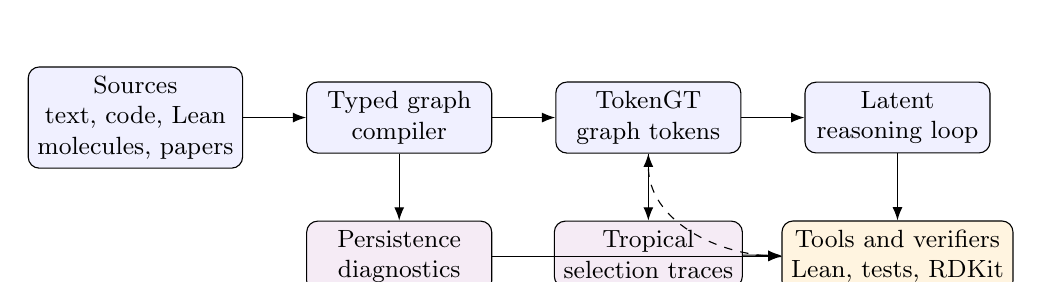
\begin{tikzpicture}[node distance=0.85cm and 0.8cm, every node/.style={font=\small}, >=Latex]
\tikzstyle{block}=[draw, rounded corners, align=center, minimum width=2.35cm, minimum height=0.75cm, fill=Blue!6]
\tikzstyle{diag}=[draw, rounded corners, align=center, minimum width=2.35cm, minimum height=0.75cm, fill=Purple!8]
\tikzstyle{tool}=[draw, rounded corners, align=center, minimum width=2.45cm, minimum height=0.75cm, fill=Orange!12]
\node[block] (src) {Sources\\text, code, Lean\\molecules, papers};
\node[block, right=of src] (graph) {Typed graph\\compiler};
\node[block, right=of graph] (tok) {TokenGT\\graph tokens};
\node[block, right=of tok] (loop) {Latent\\reasoning loop};
\node[diag, below=of graph] (topo) {Persistence\\diagnostics};
\node[diag, below=of tok] (trop) {Tropical\\selection traces};
\node[tool, below=of loop] (tools) {Tools and verifiers\\Lean, tests, RDKit};
\draw[->] (src) -- (graph);
\draw[->] (graph) -- (tok);
\draw[->] (tok) -- (loop);
\draw[->] (graph) -- (topo);
\draw[->] (tok) -- (trop);
\draw[->] (loop) -- (tools);
\draw[->] (topo) -- (tools);
\draw[->] (trop) -- (tools);
\draw[->, dashed] (tools.west) to[out=180,in=-90] (tok.south);
\end{tikzpicture}
\caption{Engineering version of the review's theoretical proposal. The key move is to turn proof states, code, biochemical mechanisms, and language structure into typed graphs, then train a small model to reason over those graphs with tool-verified trajectories.}
\label{fig:agent-engineering}
\end{figure}

\section{Four concrete exploitation strategies}
\label{sec:four-strategies}

This section gives four concrete training strategies. The first three satisfy the minimal requirement of distinct actionable model-building routes; the fourth is included because random-order graph decoding changes how the whole system should be trained.

\subsection{Strategy I: topology-gated Lean and tool-use proof agent}

The first route is a proof-and-tool agent whose training data are formalized as dependency graphs. A theorem statement becomes a graph of variables, hypotheses, types, imported definitions, candidate lemmas, tactics, and proof-state transitions. Lean acts as an unforgiving external memory and verifier: if the proof compiles, the terminal reward is positive; if it fails, the failure message is a new graph node that conditions repair.

The distinctive contribution of the paper is not simply to add Lean data. It is to add \emph{topological control}. For every proof state, construct a local dependency graph $G_t$ from active hypotheses, goals, candidate premises, imported namespaces, and tactic history. The model hidden states $H_t$ induce an embedding distogram $D_t$. Compute lightweight persistence summaries $\mathcal{P}(G_t)$ and $\mathcal{P}(H_t)$ for connected components and short cycles. A topology-gated loss penalizes hidden-state collapse when the proof state contains multiple necessary components, and it penalizes spurious fragmentation when a proof should reduce to a single chain of dependencies.

\begin{definition}[Proof-state graph]
A proof-state graph is a typed directed multigraph
\[
G_t=(V_t,E_t,\tau_V,\tau_E),
\]
where nodes include goals, local hypotheses, constants, imported theorems, tactics, error messages, generated subgoals, and natural-language comments, while edges encode type dependence, syntactic occurrence, premise retrieval, tactic application, subgoal creation, and proof repair.
\end{definition}

\begin{proposition}[Verifier-grounded graph loss]
Let $R_{\rm Lean}(\tau)$ be a terminal reward for a proof trajectory $\tau$ that is $1$ for a compiling proof and $0$ otherwise. Let $d_B$ be bottleneck or Wasserstein distance between persistence diagrams. A training objective of the form
\[
\mathcal{L}=\mathcal{L}_{\rm CE}+\lambda_1\mathcal{L}_{\rm premise}+\lambda_2\mathcal{L}_{\rm tactic}+\lambda_3 d_B(\mathcal{P}(G_t),\mathcal{P}(H_t))-\lambda_4 R_{\rm Lean}
\]
encourages the model to align latent proof geometry with formal proof-state structure while still optimizing token prediction and verifier success.
\end{proposition}

The method is especially useful for mathematics and current Lean because it separates three tasks that are often conflated: autoformalization, premise selection, and tactic synthesis \cite{Lean4Reference,LeanMathlib,LeanDojoV2}. A small model should not be asked to memorize all of mathlib. It should learn to retrieve premises, form a small active graph, propose tactics, and repair failures. This is closer to a scientific workflow than to one-shot text generation.

\subsection{Strategy II: tropical-annealed graph-of-thought with GFlowNet training}

The second route trains the agent to reason as a graph rather than as a single chain \cite{TreeOfThoughts2023,GraphOfThoughts2023,FlowOfReasoning2024,GFlowMath2025}. Chain-of-thought data are easy to collect but structurally narrow. Tree-of-thought data allow branching but not arbitrary merging. Graph-of-thought data allow a partial proof, a code experiment, a symbolic derivation, and a retrieved paper snippet to merge into one synthesis node. This matches the TokenGT premise of the paper.

Tropical geometry supplies the selection mechanism. During early training, attention and thought selection remain soft. During later training, selected heads or controller logits are annealed toward max-plus behavior:
\[
\softmax(s/\tau)\longrightarrow e_{\argmax_i s_i}\quad \text{as }\tau\to 0.
\]
The model is therefore trained to maintain a diverse graph of candidate thoughts while learning when a sharp decision is needed. The GFlowNet objective prevents the policy from collapsing onto only one high-reward path. It samples trajectories with probability proportional to terminal reward, producing multiple valid proofs, multiple algorithms, or multiple mechanistic explanations when several are acceptable.

\begin{definition}[Graph-of-thought trajectory]
A graph-of-thought trajectory is a sequence of graph states and actions, written $(S_0,a_0,\ldots,S_T)$. Each state $S_t$ is a finite typed thought graph; each action $a_t$ adds, merges, verifies, deletes, compresses, or refines nodes and edges. Terminal states carry rewards from verifiers, tests, domain constraints, or human preferences.
\end{definition}

\begin{lstlisting}[caption={GFlowNet-style graph-of-thought training loop.}]
for problem in training_stream:
    G = build_initial_problem_graph(problem)
    trajectory = []
    while not terminal(G):
        logits = controller(TokenGT(G))
        logits = tropical_anneal(logits, temperature=tau)
        action = sample_action(logits)       # expand, merge, verify, retrieve, tool-call
        G_next = apply_action(G, action)
        trajectory.append((G, action, G_next))
        G = G_next
    reward = verifier_reward(G)              # Lean, tests, unit checks, chemistry filters
    update_forward_backward_flows(trajectory, reward)
    update_supervised_heads(trajectory)
    tau = schedule(tau)
\end{lstlisting}

The novelty is the coupling of three mechanisms: TokenGT supplies graph tokens, tropical annealing supplies decisiveness, and GFlowNets supply trajectory diversity. For mathematical proof, terminal reward may be Lean success plus proof shortness and minimal imports. For code, it may be unit-test pass rate plus static analysis. For physics, it may include dimensional consistency and numerical agreement. For biochemistry, it may include assay consistency, molecular validity, toxicity filters, and mechanistic plausibility.

\subsection{Strategy III: biochemical mechanism and medicinal-design graph agent}

The third route exploits the paper's biochemical half directly. Instead of training on biomedical text as plain text, construct typed mechanism graphs. Nodes include proteins, genes, residues, domains, ligands, assays, cell types, pathways, diseases, phenotypes, concentrations, binding constants, adverse effects, and citations. Edges include \texttt{binds}, \texttt{inhibits}, \texttt{activates}, \texttt{phosphorylates}, \texttt{expressed-in}, \texttt{causes}, \texttt{contraindicated-with}, \texttt{measured-by}, and \texttt{supported-by}. Molecules are entered as molecular graphs with atom and bond tokens; proteins can be represented by sequence segments, residue graphs, predicted pockets, and text annotations.

This agent is not a clinical decision system. It is a research assistant for mechanism generation, literature-grounded hypothesis construction, assay planning, and molecular-design triage. Its central discipline is that every claim must be attached to evidence nodes and every molecular proposal must pass validity and safety screens before it is surfaced.

\begin{lstlisting}[caption={Mechanism-graph construction for biochemical and medicinal chemistry data.}]
for record in biomedical_sources:
    text_nodes = extract_entities(record.abstract_or_table)
    molecule_nodes = parse_smiles_or_inchi(record.compounds)
    protein_nodes = map_targets_to_uniprot(record.targets)
    assay_nodes = normalize_assays(record.activity_values, units=True)
    evidence_node = citation(record.source_id, record.license, record.date)
    G = typed_graph()
    G.add_nodes(text_nodes + molecule_nodes + protein_nodes + assay_nodes + [evidence_node])
    G.add_edges(entity_relations(record))          # inhibits, binds, activates, pathway links
    G.add_edges(molecular_bonds(record.compounds)) # atoms and bonds
    G.add_edges(evidence_links(evidence_node))
    G = add_safety_and_uncertainty_tags(G)
    yield serialize_tokengt_example(G)
\end{lstlisting}

The model should be trained to answer questions in the following form: ``Given a target, a disease pathway, and a set of assays, propose three mechanistically distinct hypotheses, list evidence, state missing experiments, and reject unsafe or unsupported claims.'' The graph representation forces the answer to be relational; topology summarizes pathway modules and molecular rings; tropical selection chooses candidate mechanisms; tool verification checks molecule syntax, units, simple physicochemical filters, and consistency with known assays.

\subsection{Strategy IV: random-order graph autoregression for non-canonical structures}

The fourth route addresses a foundational mismatch. Left-to-right decoding is natural for prose, but many reasoning objects have no privileged order: proof dependency graphs, molecule graphs, parse forests, semantic frames, code dependency graphs, and graph-of-thought states. A random-order autoregressive objective trains the model to fill a graph in many valid orders. This is particularly appropriate for TokenGT, where node and edge tokens are already first-class objects.

Let $Y=(y_1,\ldots,y_m)$ be the set of output graph tokens. Let $\Pi_m$ be a distribution over permutations. The random-order objective is
\[
\mathcal{L}_{\rm RO}(\theta)=\E_{\pi\sim\Pi_m}\left[\sum_{t=1}^m -\log p_\theta(y_{\pi_t}\mid x, y_{\pi_1},\ldots,y_{\pi_{t-1}}, \pi_{1:t})\right].
\]
The conditioning includes an order code and a visible-set mask. For graphs, the model may also condition on partially revealed edges, boundary nodes, and desired output type.

\begin{lemma}[Chain-rule validity under arbitrary order]
For any joint distribution $p(y_1,\ldots,y_m\mid x)$ and any permutation $\pi$, one has
\[
p(y_1,\ldots,y_m\mid x)=\prod_{t=1}^m p(y_{\pi_t}\mid x,y_{\pi_1},\ldots,y_{\pi_{t-1}}).
\]
\end{lemma}

\begin{proof}
This is the ordinary chain rule for probability applied to the reordered tuple $(y_{\pi_1},\ldots,y_{\pi_m})$. Since a permutation is a bijection, the reordered tuple contains exactly the same random variables. \qedhere
\end{proof}

\begin{proposition}[Unbiased order-averaged gradient estimate]
If $\pi$ is sampled from a fixed distribution $\Pi_m$ independently of the model's stochastic sampling and the loss is differentiable in $\theta$, then the stochastic gradient obtained from one sampled order is an unbiased estimator of $\nabla_\theta \mathcal{L}_{\rm RO}$.
\end{proposition}

\begin{proof}
Under standard dominated-convergence conditions for exchanging gradient and expectation,
\[
\nabla_\theta \mathcal{L}_{\rm RO}=\nabla_\theta \E_\pi[\ell(\theta,\pi)]=\E_\pi[\nabla_\theta \ell(\theta,\pi)].
\]
Thus sampling one $\pi$ and differentiating the corresponding loss gives an unbiased Monte Carlo estimate. \qedhere
\end{proof}

Random-order decoding is not automatically better. It complicates caching and can make streaming generation less natural. Its advantage is structural: the model learns to complete partial relational objects rather than merely continue a string. For formal proofs, it can predict a missing lemma before a preceding explanatory sentence. For code, it can generate function signatures, tests, imports, and bodies in dependency order. For medicinal chemistry, it can select target, scaffold, assay, and contraindication evidence in a graph-conditioned order.

\section{Dataset program for a TokenGT agentic reasoner}
\label{sec:dataset-program}

The dataset should be built as a staged mixture, not as one undifferentiated corpus. The model must first acquire language, code, mathematics, and scientific vocabulary; then learn graph conversion; then learn tool use; then learn verified reasoning trajectories. The tables below are intentionally prescriptive. Each source should be license-checked, deduplicated, contamination-screened against evaluation sets, and converted into a typed graph schema. The recommended sources include recent open web, mathematics, code, proof, agent, and biochemical resources \cite{FineWeb2024,Dolma2024,RedPajamaV2,OpenWebMath2023,ProofPile2,TheStackV2,OpenMathInstruct2,LeanDojo2023,LeanWorkbook2024,BigCodeBench2024,TauBench2024,OSWorld2024,ChEMBL2024,BindingDB2007}.

\subsection{Current corpus audit and expansion target for a 0.5B graph reasoner}
\label{sec:dataset-expansion-audit}

The present repository state is already nontrivial: the completed public graph corpus contains $7{,}328{,}008$ examples, approximately $1.00\times 10^9$ source graph tokens, $4.89\times 10^7$ target graph tokens, and $1.11\times 10^9$ untruncated graph-sequence tokens; the 4090-bounded public corpus contains $230{,}857$ examples. The current train-ready mixture is strongest in Hebrew text, mathematical reasoning, selected formal-proof data, sequence-first molecular records, sanitized UniGenX-style metadata rows, and public binding-affinity rows. It is weakest in four places: large-scale protein sequence-function alignment; nucleic-acid sequence/function alignment; biomedical target-selection reasoning; and explicit graph-algorithm or graph-of-thought supervision at scale. Those weaknesses matter because the proposed architecture is not a text-only language model. It is a typed graph-to-graph transducer whose most important learned skill is to transform one relational object into another.

SFM/NatureLM and UniGenX currently enter the codebase in two distinct ways. First, their reference repositories and papers provide methodology and reference vocabulary; extracted NatureLM/UniGenX tokens extend the graph vocabulary but are not counted as train/validation/test examples by themselves. Second, selected UniGenX-style public sources are used only after sequence-first sanitization: molecule rows keep SELFIES/SMILES-style strings and non-structure metadata, while coordinate and physics fields are excluded from the first training curriculum. A separate NatureLM-style public-source acquisition path now downloads and prepares official PubChem, UniProt, and RefSeq slices into graph JSONL splits. The default preparation includes the tractable public slices and records provenance; full PubChem CID-SMILES and UniProt TrEMBL are high-cardinality paths that must be enabled deliberately, and Materials Project remains API-gated unless an \texttt{MP\_API\_KEY} export is supplied.

The current model scale is approximately $0.5$B parameters and the near-term training budget is about $2$B consumed tokens, plus GFlowNet and UMA-style oracle training. This budget cannot literally reproduce the raw-token scale of recent looped latent-reasoning language models, which train from multi-trillion-token web corpora and report $7.7$T-token regimes \cite{ZhuOuro2025,FineWebEdu2024,DCLM2024,Dolma2024}. The proper target is therefore two-tiered. First, build a candidate source pool that is large enough and diverse enough to support future scaling. Second, for the $2$B-token run, select a high-density curriculum in which many tokens carry typed edges, verifiers, motifs, graph states, sequence annotations, or oracle-feedback records. The training objective is not raw token maximalism; it is high mutual information between a small number of tokens and the graph-to-graph transformations the model must learn.

The expansion should also correct a split-policy problem. Row-level SHA1 splits are suitable for generic text smoke tests and the broad public selected corpus, but they are not safe as the final policy for scientific multimodal learning. In biochemistry, the same protein family, ligand scaffold, RNA family, or target-disease relation can appear in superficially different rows. In Hebrew morphology, the same root-template family can generate many surface forms that leak across random splits. In graph-reasoning data, relabeling the same graph creates near-duplicates. Hence the expanded corpus must use entity-aware and time-aware splits, with structure-aware splits reserved for evaluation-only resources and future phases. The practical rule is staged: row-hash splits may bootstrap acquisition and smoke training, but every scientific source graduates to a split registry keyed by sequence clusters, scaffolds, RNA families, KG releases and neighborhoods, Hebrew root/template families, and graph isomorphism hashes before it is used for final validation or test claims.

The default 2026 full-run selection is capped by an operational budget of at most \(5\times 10^9\) untruncated graph-sequence tokens. The sources below were selected by expected marginal quality gain for this architecture: explicit graph-state reasoning first, then sequence/function grounding for the four scientific modalities, then verifier/tool reasoning, then a curated general-language slice. If the token guard fails after graphification, the lowest-ranked rows are reduced first; OpenAI GraphWalks remains a default source because it is the most direct available supervision for long-context graph traversal and answer-node prediction.

{\scriptsize
\setlength{\tabcolsep}{2pt}
\begin{longtable}{p{0.05\linewidth}p{0.23\linewidth}p{0.43\linewidth}p{0.20\linewidth}}
\caption{Default ranked additions for the 5B-token full selected corpus.}\\
\toprule
Rank & Source & Why selected & Control \\
\midrule
\endhead
1 & OpenAI GraphWalks & Long-context graph-state traversal, operation conditioning, frontier reasoning, and answer-node prediction. & Include by default. \\
2 & GraphWiz GraphInstruct-RFT-72K & Breadth over graph QA templates and natural-language graph instructions. & Include by default. \\
3 & PubChem10M SELFIES & High-volume molecule string coverage without structure-file inputs. & Cap at 8M rows. \\
4 & UniProt function text descriptions & Protein sequence-to-function grounding for function-description outputs. & Include by default. \\
5 & Rfam & RNA family sequence and family/clan annotation. & Cap at 1M rows. \\
6 & RNAcentral 8192 & Broad RNA sequence diversity with type/description metadata. & Cap at 500k rows. \\
7 & DNA coding regions & DNA sequence, exon/intron, and translated-protein annotations. & Cap at 500k rows. \\
8 & OpenMathReasoning TIR & Tool-integrated mathematical reasoning and verifier-like traces. & Cap at 1.3M rows. \\
9 & OpenMathReasoning GenSelect & Solution-selection supervision for ranking and diversity-quality tradeoffs. & Cap at 300k rows. \\
10 & DCLM baseline 1B slice & Curated general language and fluency support without pulling a multi-trillion-token corpus. & Lowest-priority active addition. \\
\bottomrule
\end{longtable}}

\subsection{Additional datasets and source families for the next corpus expansion}
\label{sec:additional-datasets}

The dataset table below lists recommended additions beyond the current train-ready selected public corpus. Some rows are training sources; some are reference vocabularies; some are evaluation-only benchmarks that must be excluded from training. Every training source is converted to a typed graph-to-graph record: an input graph $X$ containing text, sequence, SELFIES/SMILES, proof, graph-walk, tool, oracle, or evidence records, and an output graph $Y$ containing reasoning states, function descriptions, tool traces, labels, candidate strings, oracle feedback, or target-selection justifications. Sequence renderings, SELFIES strings, FASTA files, TSV tables, and tool transcripts are serializers, not primitive targets; PDB/mmCIF/SDF and dynamics files remain evaluation-only unless a later phase explicitly permits them.

{\scriptsize
\setlength{\tabcolsep}{2pt}
\begin{longtable}{p{0.17\linewidth}p{0.16\linewidth}p{0.36\linewidth}p{0.22\linewidth}}
\caption{Additional dataset sources and how to weave them into the TokenGT graph-to-graph training program. Sources marked ``evaluation only'' should be reserved for validation or final testing.}\\
\toprule
Source & Role & Graph-to-graph adaptation & Leakage-aware split \\
\midrule
\endhead
FineWeb-Edu \cite{FineWebEdu2024} & High-quality language pool & Use only science, math, biomedical, Hebrew, and technical slices after decontamination. Convert equations, citations, definitions, and claims to text-evidence graphs. & Document-hash and URL-domain split; remove benchmark n-grams and near-duplicates. \\
DCLM baseline corpus \cite{DCLM2024} & Large candidate web pool & Use as filtered background language for robustness, not as the core scientific corpus. Sample by graph-density score. & URL/time split; MinHash and embedding decontamination against evaluation sets. \\
Dolma \cite{Dolma2024} & Mixed open pretraining pool & Adds code, web, books, papers, and reference-like text for the 0.5B model's broad language substrate. & Preserve source labels; split by document family and time when available. \\
OpenAI GraphWalks \cite{GraphWalks2026} & Long-context graph reasoning & Encode edge lists, operation tokens, frontier states, visited sets, and answers as graph records. Train random-order graph completion and GoT frontier expansion. & Split by graph generator seed, graph size, and canonical graph hash; include larger OOD graph sizes for test. \\
GraphInstruct / GraphWiz \cite{GraphInstruct2024} & Instructional graph reasoning & Convert graph QA tasks to typed node/edge/query/answer graphs. Add verifier nodes for shortest path, connectivity, matching, and centrality. & Split by graph isomorphism hash and task template; avoid node-renaming leakage. \\
NLGraph \cite{NLGraph2023} & Natural-language graph tasks & Convert natural-language graph problems into explicit graph states, then back into answers and explanations. & Hold out graph families and graph sizes; test on unseen operations. \\
G1/Erdos graph reasoning \cite{ErdosGraphReasoning2025} & Synthetic graph algorithm QA & Use as high-volume graph-algorithm pretraining for BFS, cycle, topological-order, and reachability records. & Split by generator seed, canonical graph hash, and OOD size. \\
CLRS and CLRS-Text \cite{CLRS2022,CLRSText2024} & Algorithmic reasoning with traces & Treat algorithm hints as intermediate GoT states. Train vertex labels, edge relaxations, priority queues, and final outputs. & Split by algorithm, graph size, and seed; reserve unseen algorithm-size pairs. \\
ThoughtSource \cite{ThoughtSource2023} & CoT/ToT trace normalization & Use as a trace source only after converting chains into DAGs of claims, subgoals, and dependencies. Prefer verified traces. & Split by original dataset and problem identity; decontaminate against math and science evals. \\
SciRIFF \cite{SciRIFF2024} & Scientific instruction following & Convert literature tasks into paper-claim-evidence graphs for extraction, QA, claim verification, and summarization. & Split by paper DOI/arXiv identifier and task family. \\
SciInstruct \cite{SciInstruct2024} & General scientific instruction & Adds chemistry, biology, math, and verifier-checkable scientific explanations. Convert to typed problem-solution-verifier graphs; exclude direct simulation or dynamics data. & Split by source document and problem template. \\
BioInstruct \cite{BioInstruct2023} & Biomedical instruction & Adds biomedical QA, extraction, and explanation tasks. Convert entities, relations, and evidence spans into biomedical reasoning graphs. & Split by PubMed ID, entity pair, and relation type. \\
PubMedQA / BioASQ-style sources \cite{PubMedQA2019,BioASQ2024} & Biomedical question answering & Convert question, abstract snippets, MeSH entities, answer, and evidence into graph records. Use mainly for supervised biomedical reasoning. & Split by article identifier and disease/target families. \\
FutureHouse LAB-Bench and LAB-Bench 2 \cite{LABBench2024,LABBench2_2026} & Biology-agent evaluation & Evaluation only. Use for tool-augmented biology reasoning, literature lookup, and protocol understanding. & Never train on benchmark questions; use as held-out assessment. \\
FutureHouse BixBench and HLE Bio/Chem Gold \cite{BixBench2025,HLEBioChemGold2026} & Research-agent evaluation & Evaluation only. Use to test whether graph reasoning transfers to expert biology/chemistry tasks. & Exclude prompts and solutions from training; use benchmark contamination screens. \\
Open Targets Platform \cite{OpenTargets2026} & Target-selection reasoning & Build disease-target-evidence graphs with genetics, literature, pathway, tractability, safety, and druggability nodes. Train target-prioritization GoT traces. & Time-split by platform release; hold out disease families and target families. \\
Open Targets clinical evidence \cite{OpenTargetsClinicalEvidence2026} & Clinical evidence grounding & Add trial, indication, target, drug, phase, and outcome edges; train evidence-weighted explanation graphs. & Temporal split by trial date and target/indication clusters. \\
Therapeutics Data Commons \cite{TDC2021} & Drug-discovery task suite & Convert ADMET, drug-target, molecule generation, and therapy tasks into molecule-target-property graphs. & Use official splits when appropriate; otherwise scaffold, target-family, or time splits. \\
PrimeKG \cite{PrimeKG2023} & Precision-medicine KG & Add disease-gene-drug-pathway-phenotype relations for multihop mechanism reasoning and GFlowNet path sampling. & Relation-aware splits; hold out disease families and target neighborhoods. \\
Hetionet \cite{Hetionet2017} & Biomedical KG & Use as an interpretable biomedical path-reasoning source and baseline KG for drug repurposing explanations. & Node-pair and relation-type splits; remove inverse-edge leakage. \\
OpenBioLink \cite{OpenBioLink2020} & Biomedical link prediction & Train link prediction, path explanation, and negative-edge discrimination over biomedical relations. & Use release-defined train/valid/test; audit negative sampling leakage. \\
STRING \cite{STRING2023} & Protein interaction graph & Build protein-protein interaction, confidence, organism, and evidence-channel graphs. & Species-aware and family-aware splits; hold out interaction neighborhoods. \\
ProTrek-style resources \cite{ProTrek2025} & Sequence-function alignment & Use sequence and function descriptions as contrastive graphs in the first curriculum; structure fields are reserved for evaluation-only retrieval audits. Convert retrieval positives and hard negatives into graph pairs. & Split by sequence identity; hold out protein families and audit structural similarity only in evaluation. \\
UniProt family resources \cite{UniProt2025,UniRef2025} & Protein function text and sequences & Pair amino-acid sequence graphs with curated function, GO, EC, disease, subcellular-location, and feature annotations. & Cluster by UniRef50/UniRef30; temporal split by release; keep all isoforms together. \\
ProteinGym \cite{ProteinGym2023} & Mutational fitness landscapes & Convert wild type, mutation set, assay condition, and measured score into sequence-function graphs. & Protein-family and assay-level holdout; never split variants of one assay across train/test. \\
PEER \cite{PEER2022} & Protein representation benchmark suite & Use training partitions for protein function, localization, interaction, and sequence-backed ligand tasks. Structure-specific tasks are evaluation-only in the first run. & Respect benchmark splits; add family-level holdouts for transfer tests. \\
FLIP and FLIP2 \cite{FLIP2021,FLIP2_2026} & Protein engineering tasks & Train design and property reasoning over realistic protein-engineering splits. & Use published split logic; hold out families and assay campaigns. \\
RCSB/wwPDB + AlphaFold DB \cite{RCSBPDB2026,wwPDB2026,AlphaFoldDB2026} & Evaluation-only structure resources & Use for contamination audits, external validation, and future structure-phase design; do not train first-run models on atom, coordinate, or distogram records. & Temporal PDB split, sequence cluster split, structure cluster split; no homolog leakage. \\
PDBbind / PDBbind+ \cite{PDBbind2021,PDBbindPlus2026} & Evaluation-only protein-ligand resources & Use for held-out biochemical validation and future structure-conditioned experiments; first-run training uses sequence/string assay metadata only. & Split by ligand scaffold and protein family; reserve refined/core-style sets. \\
GEOM, SPICE, PCQM4Mv2, PubChemQC \cite{AxelrodGEOM2022,EastmanSPICE2023,PCQM4Mv2,PubChemQC2023} & Molecule strings and evaluation-only physics labels & Use SELFIES/SMILES, identifiers, and non-structure properties when allowed; conformers, coordinates, energies, and forces are excluded from first-run training. & Bemis-Murcko scaffold and InChIKey-block splits; conformers of the same molecule stay together for evaluation. \\
OMol25/UMA resources \cite{LevineOMol25_2025,WoodUMA2025} & External oracle and evaluation & Use UMA-style systems to score model-generated candidate graph states and emit binned oracle feedback; do not train directly on OMol25 energy-force snapshots in the first run. & Split by chemical system and benchmark for evaluation; avoid near-duplicate structures. \\
mdCATH, ATLAS, MD22 \cite{MirarchiMdCATH2024,VanderMeerscheATLAS2024,MD22_2022} & Evaluation-only dynamics resources & Reserve for later structure/dynamics validation and future-phase experiments; do not train first-run models on trajectories, displacements, or force bins. & Protein-domain, molecule-system, and temperature-replica splits; hold out full trajectories. \\
RNAcentral and Rfam \cite{RNAcentral2024,Rfam2025} & RNA sequence, family, and covariance & Build RNA sequence, motif, family, covariance, secondary-structure, and function graphs. & Rfam-family and covariance-model splits; sequence-identity filters. \\
NAKB, RNA 3D Hub, RNA3DB \cite{NAKB2024,RNA3DHub2025,RNA3DB2024} & Evaluation-only nucleic-acid structures & Reserve base-pair, stacking, loop, motif, ion, ligand, and coordinate records for validation and future phases. & Structure-dissimilar splits; hold out motif families and PDB release periods. \\
Reference genome resources \cite{NCBINucleotide2026,GenBank2026,Ensembl2026,GENCODE2026} & DNA/RNA annotation & Convert genomic intervals, transcripts, genes, exons, regulatory annotations, and product descriptions into sequence-feature graphs. & Split by chromosome, gene family, taxon, and release date. \\
UniMorph Hebrew \cite{UniMorph2024,UniMorphHebrew2026} & Hebrew morphology & Build root-template-lemma-feature-surface graphs; use inflectional paradigms as branching graph outputs. & Hold out roots and templates, not individual forms. \\
Hspell and MILA/YAP Hebrew resources \cite{Hspell2026,MILA2008,YAP2026} & Hebrew analyzers and lexica & Use analyzers to produce candidate roots, binyanim, diacritized forms, and morphological features. Train parser-agreement graphs. & Split by root, binyan, lexical family, and genre; respect license restrictions. \\
UD Hebrew and Hebrew QA resources \cite{UDHebrewIAHLT2026,HebrewQANLP2024} & Hebrew syntax and QA & Convert dependency trees, QA spans, entities, and answer justifications to graph-to-graph examples. & Split by document and root family; avoid same sentence variants across splits. \\
Open Multilingual WordNet and Hebrew corpora \cite{OpenMultilingualWordNet2012,HebrewCHILDES2013} & Hebrew semantic analogues & Build synset, translation, child-language, morphology, and semantic-neighborhood graphs for Hebrew analogues of English reasoning. & Hold out synsets and root families; genre/time split for corpora. \\
\bottomrule
\end{longtable}}

\subsection{Converting the expanded sources into GoT, ToT, CoT, and GFlowNet training}
\label{sec:gflow-dataset-conversion}

The preferred supervision order is graph-of-thought, then tree-of-thought, then chain-of-thought. A chain is a special case of a tree, and a tree is a special case of a directed acyclic thought graph. Therefore the curator should first attempt to build a typed directed acyclic graph of intermediate states. Only when the source lacks enough relational structure should it fall back to tree or chain supervision.

For a source graph $G_0$ and target object $Y$, define a reasoning trajectory as a sequence of partial graph states
\[
S_0\to S_1\to\cdots\to S_T,
\]
where $S_t$ is a typed subgraph containing selected evidence, hypotheses, tool calls, intermediate computations, and unresolved frontier nodes. The terminal reward is not a scalar accuracy flag alone. For scientific tasks it should combine validity, evidence support, novelty control, physical plausibility, and decontamination status:
\[
R(S_T)=\exp\{\alpha A+\beta V+\gamma E-\delta C-\eta L\}.
\]
Here $A$ is task accuracy, $V$ is verifier success, $E$ is evidence support, $C$ is contradiction or chemical invalidity, and $L$ is leakage or provenance penalty. A GFlowNet then learns to sample high-reward graph-construction trajectories rather than one canonical explanation \cite{BengioGFlowFoundations2023,FlowOfReasoning2024,GFlowMath2025}.

\begin{lstlisting}[caption={Generic conversion of a source into graph-of-thought and GFlowNet records.}]
def curate_got_gfn_records(raw_example, source_config):
    X = graphify_input(raw_example, source_config.schema)
    candidates = propose_intermediate_states(X, source_config)
    states = []
    for c in candidates:
        S = canonicalize_typed_graph(c)
        S.verifier = run_verifiers(S, raw_example)
        S.evidence = attach_evidence_nodes(S, raw_example)
        states.append(S)
    edges = infer_state_transitions(states)
    terminal = select_terminal_states(states, edges)
    reward = compute_reward(terminal,
                            accuracy=task_score(terminal),
                            validity=verifier_score(terminal),
                            evidence=evidence_score(terminal),
                            contradiction=contradiction_penalty(terminal),
                            leakage=leakage_penalty(raw_example))
    return GraphTrajectory(X=X, states=states, edges=edges,
                           terminal=terminal, reward=reward)
\end{lstlisting}

Open Targets is a central example. A disease-target pair becomes a terminal target-selection hypothesis; genetics, somatic mutation, literature, animal model, pathway, tractability, safety, druggability, and clinical-evidence records become evidence nodes. A GoT trace is a subgraph that explains why a target should be prioritized or rejected. A GFlowNet policy samples alternative evidence paths, and the reward combines platform association score, evidence diversity, novelty, safety penalties, and whether the path can be independently reconstructed from source tables.

\begin{lstlisting}[caption={Open Targets disease-target evidence graph to GoT/GFlowNet trajectory.}]
def open_targets_to_target_selection(row, release_tables):
    X = Graph()
    disease = X.node("disease", row.disease_id)
    target = X.node("target", row.target_id)
    X.edge(disease, target, kind="candidate_target")
    for ev in load_evidence(row, release_tables):
        e = X.node("evidence", ev.id,
                   source=ev.datasource,
                   score=ev.score,
                   date=ev.date)
        X.edge(e, disease, kind="supports_disease_context")
        X.edge(e, target, kind="supports_target")
    S0 = X.subgraph([disease, target])
    trajectories = sample_evidence_expansions(X, start=S0,
                                              actions=["add_genetics",
                                                       "add_pathway",
                                                       "add_safety",
                                                       "add_clinical",
                                                       "reject_weak"])
    for tr in trajectories:
        tr.reward = target_reward(tr,
                                  association=row.association_score,
                                  evidence_diversity=count_sources(tr),
                                  safety_penalty=safety_flags(tr),
                                  provenance_ok=all_edges_reproducible(tr))
    return trajectories
\end{lstlisting}

For ProTrek-style sequence-function data in the first curriculum, the trajectory is contrastive: the model observes a protein sequence graph or a function-description graph and must retrieve or generate the matching graph in another modality. Hard negatives are created by choosing same-family but different-function proteins or same-GO-term but different-domain architectures. Structure-motif variants are reserved for evaluation-only audits and later explicit phases. This yields graph-to-graph retrieval and generation data without forcing all supervision into a sequence continuation objective.

For graph-algorithm sources such as GraphWalks and CLRS, each algorithm execution already has a natural frontier process. BFS states contain a queue, visited set, and frontier edges; shortest-path states contain tentative distances and predecessor edges; topological-sort states contain in-degree records and emitted nodes. These should be stored as intermediate graph states rather than verbal rationales. For Hebrew, a root graph begins at a consonantal root and expands through binyan/template, diacritization, lemma, surface form, part of speech, syntactic dependency, and semantic-neighborhood nodes. The reward is parser agreement, lexicon support, corpus attestation, and semantic coherence.

\subsection{Entity-aware and time-aware splitting}
\label{sec:entity-aware-splits}

The expanded corpus should replace generic row-level splitting with a typed split registry. Each training example receives one or more split keys: protein sequence cluster, ligand scaffold, InChIKey block, RNA family, KG release date, disease family, target family, Hebrew root, Hebrew template, graph generator seed, graph canonical hash, source document identifier, and benchmark-contamination hash. Evaluation-only structure resources additionally receive structure cluster keys for audit reports. The split is a function of the strongest leakage key, not simply the row identifier.

\begin{lstlisting}[caption={Entity-aware split assignment for multimodal graph examples.}]
def assign_split(example, split_config):
    keys = []
    if example.has_protein_sequence:
        keys.append(mmseqs_cluster(example.protein_sequence, threshold=0.30))
        keys.append(uniref_cluster(example.protein_id, level="UniRef50"))
    if example.has_protein_structure and example.is_evaluation_only:
        keys.append(foldseek_cluster(example.structure_id, threshold="remote_homology"))
        keys.append(cath_or_ecod_family(example.structure_id))
    if example.has_molecule:
        keys.append(bemis_murcko_scaffold(example.molecule))
        keys.append(inchikey_first_block(example.molecule))
    if example.has_rna:
        keys.append(rfam_family(example.rna_id))
        if example.is_evaluation_only:
            keys.append(rna3d_structural_cluster(example.structure_id))
    if example.has_kg_edges:
        keys.append((example.kg_release, example.disease_family, example.target_family))
    if example.language == "hebrew":
        keys.append((example.root, example.binyan, example.template))
    if example.has_algorithm_graph:
        keys.append(canonical_graph_hash(example.graph, ignore_node_names=True))
    key = strongest_available_key(keys)
    return deterministic_bucket(key, split_config)
\end{lstlisting}

For proteins, the strictest first-run training split should hold out sequence neighborhoods; evaluation-only structure audits additionally verify that no train sequence has a near-homologous structure in a reported held-out structure benchmark. For molecules, scaffold holdout and InChIKey-block grouping are the main tests, and conformers of one molecule must stay together in evaluation-only resources. For RNA, Rfam-family splits are more meaningful than row-level splits, with RNA3DB-style structural dissimilarity used only for structure-side evaluation. For biomedical KGs, a time split is essential: train on one Open Targets or KG release, validate on a later release, and test on edges or disease-target pairs newly supported in still later releases. For Hebrew, all common inflections of a root-template family should be assigned to the same split; otherwise the model can memorize a paradigm and appear to generalize.

\subsection{Recommended 2B-token curriculum for the 0.5B model}
\label{sec:two-billion-curriculum}

The curriculum table below gives a concrete consumed-token allocation. The point is not to exhaust every dataset. It is to create a balanced graph-dense run that can be trained on modest hardware while preserving enough scientific, graph, and language diversity to support the architecture. The same source pool can later be resampled for larger training runs.

{\scriptsize
\setlength{\tabcolsep}{2pt}
\begin{longtable}{p{0.20\linewidth}p{0.09\linewidth}p{0.43\linewidth}p{0.20\linewidth}}
\caption{Suggested $2$B-token high-density curriculum for the current $0.5$B-parameter model. Percentages are consumed training tokens, not source-corpus sizes.}\\
\toprule
Mixture block & Share & Main sources & Primary supervision \\
\midrule
\endhead
Filtered language, science, and Hebrew text & 20\% & FineWeb-Edu, Dolma, DCLM slices, SciRIFF, SciInstruct, Sefaria/Wikipedia Hebrew after filtering & Graphified text, claims, definitions, evidence, morphology. \\
Math, code, and formal proof & 15\% & OpenMathInstruct-2, NuminaMath, Lean Workbook, LeanDojo, BigCodeBench, The Stack v2 permissive slices & Proof-state graphs, code dependency graphs, test/repair traces. \\
Graph algorithms and GoT reasoning & 12\% & GraphWalks, GraphInstruct, NLGraph, Erdos/G1, CLRS, CLRS-Text, synthetic verifier traces & Frontier graphs, algorithm states, random-order graph completion, GFlowNet trajectories. \\
Protein sequence-function & 18\% & UniProt/UniRef, ProTrek-style sequence-function resources, ProteinGym, PEER, FLIP & Sequence, motif, function, mutation, annotation, and retrieval graphs. \\
SELFIES, ligands, molecules, and binding & 14\% & ChEMBL, BindingDB, PubChem/PubChemQC identifiers, PCQM4Mv2 strings, MoleculeNet & SELFIES/SMILES, scaffold, assay, affinity, property, validator, and repair graphs. \\
DNA/RNA sequence and annotation & 7\% & RNAcentral, Rfam, RefSeq, GenBank, Ensembl/GENCODE & Nucleotide, family, motif, transcript, annotation, and sequence-function graphs. \\
Biomedical KG and target selection & 9\% & Open Targets, TDC, PrimeKG, Hetionet, OpenBioLink, STRING, clinical evidence tables & Disease-target-evidence GoT, mechanism paths, link prediction, target-prioritization reward. \\
Oracle conditioning and GFlowNet rewards & 4\% & UMA-style oracle calls, validators, generated SELFIES/sequence candidate graph states & Temperature tokens, oracle reward bins, verifier feedback, and graph-state trajectories. \\
Hebrew root-graph specialization & 1\% & UniMorph Hebrew, Hspell, MILA/YAP, UD Hebrew, Hebrew QA, OMW/Hebrew resources & Root-template-lemma-surface graphs and Hebrew analogues of reasoning tasks. \\
\bottomrule
\end{longtable}}

This allocation intentionally gives graph reasoning a large share relative to its raw token availability. A 0.5B model should overtrain on the transformations that define its intended use: graph traversal, proof-state transition, biochemical evidence aggregation from sequence/string records, temperature-conditioned oracle reasoning, and random-order completion of relational objects.

\subsection{Validation and ablation plan for the expanded dataset}
\label{sec:expanded-validation}

The expanded dataset should be validated before expensive training. Validation is not only final model evaluation; it is also a corpus-quality audit. The validation table below gives the minimum tests that should be run after graphification and before the full training run.

{\scriptsize
\setlength{\tabcolsep}{3pt}
\begin{longtable}{p{0.19\linewidth}p{0.32\linewidth}p{0.23\linewidth}p{0.15\linewidth}}
\caption{Empty validation and ablation table for the expanded corpus.}\\
\toprule
Validation block & Required test & Metric & Result \\
\midrule
\endhead
Split leakage audit & Protein sequence, molecule scaffold, RNA family, KG time, Hebrew root, graph hash & Max train-test similarity; duplicate rate & \emph{To be filled} \\
GraphWalks/CLRS transfer & Train on smaller graphs, test on larger and differently distributed graphs & Accuracy by operation and graph size & \emph{To be filled} \\
GoT versus ToT versus CoT & Same tasks trained with graph, tree, and chain traces & Accuracy, verifier pass rate, trajectory diversity & \emph{To be filled} \\
Open Targets target selection & Reconstruct held-out disease-target evidence paths from later releases & AUROC, AUPRC, evidence-path precision & \emph{To be filled} \\
Protein sequence-function retrieval & Retrieve function from sequence and sequence families from function & Recall@k, family-heldout accuracy & \emph{To be filled} \\
Protein mutational generalization & ProteinGym/FLIP heldout proteins and assays & Spearman, NDCG, top-k enrichment & \emph{To be filled} \\
Molecular scaffold generalization & Heldout scaffolds from ChEMBL/PubChem/MoleculeNet & Validity, property accuracy, oracle reward rank & \emph{To be filled} \\
RNA family generalization & Heldout Rfam families and sequence motifs & Family F1, motif accuracy, sequence annotation accuracy & \emph{To be filled} \\
UMA oracle conditioning & Temperature-conditioned candidate graph search & Oracle reward rank correlation, diversity, calls per success & \emph{To be filled} \\
Hebrew root transfer & Heldout roots/templates and genre-shifted corpora & Morphological accuracy, root recovery, QA F1 & \emph{To be filled} \\
Benchmark contamination & LAB-Bench, BixBench, HLE Bio/Chem Gold, graph-reasoning benchmarks & Near-duplicate and embedding-similarity hits & \emph{To be filled} \\
\bottomrule
\end{longtable}}

\subsection{Dataset construction details for replication}
\label{sec:dataset-replication-details}

A reproducible implementation should store all examples in a unified record format with fields
\[
(\texttt{source\_id},\texttt{release},\texttt{license},\texttt{split\_key},X,Y,\texttt{verifiers},\texttt{provenance}).
\]
The graph $X$ is the conditioning object; $Y$ is the output graph. For next-token rendering, $Y$ may be serialized to text, Lean, SELFIES, FASTA, PDB, SDF, or JSON, but the training and split logic should remain graph-native. All motif vocabularies, scaffold clusters, sequence clusters, and root-template inventories must be mined from training data only; validation and test motifs may be mapped to an \texttt{UNK\_MOTIF} or to a coarser ontology token.

\begin{lstlisting}[caption={End-to-end source expansion and graphification pipeline.}]
def build_expanded_corpus(source_specs, split_config, token_budget):
    raw = []
    for spec in source_specs:
        data = download_or_load(spec)
        assert license_is_allowed(data.license, spec.use)
        data = normalize_release_and_provenance(data)
        raw.extend(data)

    graph_examples = []
    for ex in raw:
        X, Y = graphify_to_input_output(ex)
        split = assign_split(ex, split_config)
        leak = contamination_screen(X, Y, benchmark_registry())
        quality = graph_density_score(X, Y) + verifier_score(X, Y) - leak.penalty
        graph_examples.append((X, Y, split, quality, provenance(ex)))

    graph_examples = deduplicate_by_graph_hash(graph_examples)
    graph_examples = remove_cross_split_leakage(graph_examples)
    curriculum = stratified_quality_sample(graph_examples,
                                           token_budget=token_budget,
                                           mixture=TARGET_MIXTURE)
    write_manifest(curriculum)
    write_integrity_report(curriculum)
    return curriculum
\end{lstlisting}

For evaluation-only biological structure sources, the same function must keep all conformers, all temperature frames, and all oracle-relaxed variants of one molecule or biomolecular complex within one split and must mark those rows as excluded from first-run training. For KG sources, it must materialize a release-time view of the graph before forming evidence paths. For Hebrew, it must group by root and template before sampling. For GraphWalks and CLRS-style data, it must canonicalize graph isomorphism classes; node relabelings are augmentations, not independent test examples.



\subsection{Pretraining mixture}

\begin{longtable}{p{0.18\linewidth}p{0.30\linewidth}p{0.38\linewidth}}
\caption{Recommended public pretraining sources and their function in the proposed agent.}\label{tab:pretrain-sources}\\
\toprule
Data class & Candidate public sources & Use in the TokenGT agent\\
\midrule
General high-quality web & FineWeb, FineWeb-Edu, Dolma, RedPajama-V2 & Basic language, broad facts, style diversity, instruction substrate. Use only heavily filtered slices for a small model.\\
Mathematical web and papers & OpenWebMath, Proof-Pile-2, arXiv mathematics slices & LaTeX, theorem statements, derivations, definitions, expository proof style. Convert equations and citations to graph nodes.\\
Code & The Stack v2, permissively licensed GitHub slices, package documentation, unit-test corpora & Programming syntax, APIs, dependencies, test-driven repair. Construct import-call-test graphs.\\
Formal proof & mathlib, LeanDojo traces, Lean Workbook, MiniF2F, ProofNet, PutnamBench & Verified proof states, tactic graphs, autoformalization, premise retrieval, proof repair.\\
Verifier-guided scientific reasoning & Textbook-style unit-analysis problems, theorem-like physical laws, curated symbolic checks & Dimensional reasoning, symbolic derivation, and verifier records only; no direct physics simulation or dynamics datasets in the first training run.\\
Biomedical and chemistry & PubMed/PMC permitted subsets, ChEMBL, BindingDB, MoleculeNet, PubChem/UniProt annotations & Mechanism graphs, ligand-target relationships, assay normalization, SELFIES/SMILES validity, biomedical literature grounding.\\
Agentic tool use & Tool-call transcripts constructed from Python, Lean, shell, retrieval, RDKit, notebooks; tau-bench and OSWorld-like tasks for evaluation & Teaches the model to decide when to call tools, how to read outputs, and how to repair plans.\\
\bottomrule
\end{longtable}

For a single 4090, one should not try to ingest all of these at scale. The better approach is \emph{quality- and graph-density-weighted sampling}: prefer examples with explicit equations, typed dependencies, verifiable claims, compilable code, formal statements, assay values, or graph extractability. A small model benefits more from a million excellent graph-rich examples than from billions of weakly filtered tokens.

\subsection{Reasoning and instruction mixture}

\begin{longtable}{p{0.18\linewidth}p{0.24\linewidth}p{0.40\linewidth}}
\caption{Instruction and reasoning datasets to convert into graph, tree, and verifier traces.}\label{tab:reasoning-sources}\\
\toprule
Skill & Sources and construction methods & Graph conversion and supervision\\
\midrule
Mathematical reasoning & NuminaMath-CoT, NuminaMath-TIR, OpenMathInstruct-2, OpenMathReasoning, problem generators with symbolic verification & Convert solution steps to nodes; mark algebraic dependencies; attach Python or CAS verification when available.\\
Formal proof & Lean Workbook, Goedel-LM Lean proof traces, LeanDojo, MiniF2F, ProofNet, PutnamBench, mathlib dependency extraction & Convert theorem statements, tactic states, imports, premises, errors, and repairs into proof-state graphs.\\
Code and technical tools & The Stack v2, BigCodeBench-style tasks, package documentation, unit tests, synthetic bug-fix traces & Convert files, imports, functions, calls, tests, and failure messages into dependency graphs.\\
Agent behavior & tau-bench-style policy/API interactions, OSWorld-style computer tasks, custom laboratory and theorem-proving tasks & Convert policy rules, tool schemas, user goals, state changes, and final database or environment checks into action graphs.\\
Verifier-guided scientific reasoning & Curated unit-analysis problems, symbolic derivations, dimensional-analysis generators, and independently checkable explanations & Enforce units as typed nodes; verify dimensions and numerical answers without training on direct simulation/physics datasets.\\
Biochemistry and medicinal design & ChEMBL/BindingDB records, MoleculeNet labels, literature-grounded mechanism extraction, RDKit-valid SELFIES/SMILES molecules & Convert assays, targets, ligands, pathways, evidence, contraindications, and uncertainty to typed mechanism graphs.\\
\bottomrule
\end{longtable}

\subsection{Codex-synthetic reasoning traces}

The request for datasets from Codex 5.3, 5.4, and 5.5 should be interpreted precisely. At the time of writing, the relevant OpenAI products are model services and agentic coding systems, not public downloadable datasets \cite{OpenAICodexModels2026,OpenAIGPT55}. Therefore a scientifically clean paper should not claim the existence of open ``Codex 5.3/5.4/5.5 datasets'' unless such corpora are actually released. What can be specified is a reproducible \emph{Codex-synthetic trace methodology}: use available strong teacher models, subject to terms, privacy constraints, and provenance logging, to generate candidate traces; then filter those traces with independent verifiers.

A high-quality Codex-synthetic pipeline should satisfy five rules.

\begin{enumerate}
\item \textbf{Verifier first.} Never trust teacher reasoning text by itself. Keep only traces that pass Lean, unit tests, numerical checks, molecule validity checks, or independent critic review.
\item \textbf{Diversity by construction.} For each problem, request chain, tree, and graph variants; include failed attempts and repairs when they are informative.
\item \textbf{No benchmark leakage.} Hash and semantically screen prompts and outputs against validation and test sets before training.
\item \textbf{Provenance labels.} Store teacher model, date, prompt template, verifier outcome, license status, and decontamination status.
\item \textbf{Student compression.} Train the small model on the verified graph, tool-call, and repair structure, not on verbose teacher style.
\end{enumerate}

\begin{lstlisting}[caption={Codex-synthetic trace generation with independent verification.}]
for task in seed_tasks:
    prompt = make_teacher_prompt(task, require_graph=True, require_tool_plan=True)
    candidates = []
    for teacher in TEACHER_MODELS:        # e.g., available Codex/GPT teachers
        for mode in ["chain", "tree", "graph", "random_order"]:
            trace = teacher_generate(prompt, mode=mode, temperature=sample_temp(mode))
            graph = parse_trace_to_typed_graph(trace)
            result = run_independent_verifiers(task, graph)
            candidates.append((graph, result, provenance(teacher, mode)))
    kept = select_diverse_verified(candidates,
                                   require_no_test_leakage=True,
                                   require_license_ok=True)
    write_jsonl(kept)
\end{lstlisting}

The purpose of the teacher is not to provide ground truth. The purpose is to propose diverse paths that independent verifiers can accept, reject, or partially repair. This distinction is crucial for publication-quality rigor.

\section{Random-order autoregressive graph decoding}
\label{sec:random-order-decoding}

Random-order decoding generalizes left-to-right decoding by making the generation order a latent or sampled variable. In a graph language model, output order should often be induced by dependency, uncertainty, or verifier strategy rather than by surface text position.

\begin{definition}[Visible-set mask]
Let $Y$ be a set of output graph tokens. At step $t$ under order $\pi$, the visible set is $V_t=\{y_{\pi_1},\ldots,y_{\pi_{t-1}}\}$. A visible-set mask permits attention from the prediction query to $x\cup V_t$ and blocks attention to unrevealed target tokens. For edge prediction, the mask may expose endpoint placeholders while hiding labels.
\end{definition}

The model has two position systems. A \emph{structural position} gives graph distance, edge type, file path, proof-state namespace, or molecule atom index. A \emph{generation position} gives reveal order. This is analogous in spirit to permutation language modeling and more recent any-order autoregressive models, but the graph setting requires typed masks and verifier-aware actions \cite{XLNet2019,SigmaGPT2024,RandAR2025}.

\begin{figure}[H]
\centering
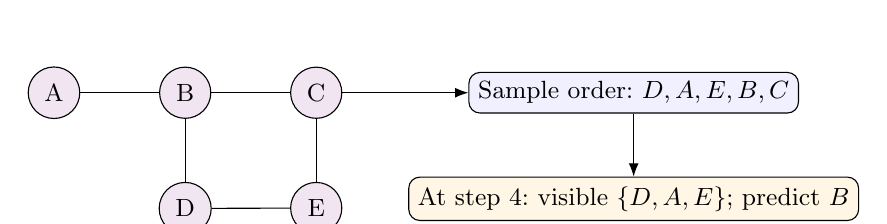
\begin{tikzpicture}[node distance=0.85cm, every node/.style={font=\small}, >=Latex]
\tikzstyle{tok}=[circle, draw, minimum size=0.65cm, fill=Purple!10]
\node[tok] (a) {A};
\node[tok, right=1.0cm of a] (b) {B};
\node[tok, right=1.0cm of b] (c) {C};
\node[tok, below=0.8cm of b] (d) {D};
\node[tok, below=0.8cm of c] (e) {E};
\draw[-] (a)--(b); \draw[-] (b)--(c); \draw[-] (b)--(d); \draw[-] (c)--(e); \draw[-] (d)--(e);
\node[draw, rounded corners, fill=Blue!6, right=1.6cm of c, align=center] (ord) {Sample order:\ $D,A,E,B,C$};
\node[draw, rounded corners, fill=Orange!10, below=0.8cm of ord, align=center] (mask) {At step 4:\ visible $\{D,A,E\}$;\ predict $B$};
\draw[->] (c) -- (ord);
\draw[->] (ord) -- (mask);
\end{tikzpicture}
\caption{Random-order graph autoregression. The graph has structural edges independent of the reveal order. Training samples many reveal orders so the model learns to complete partial relational objects.}
\label{fig:random-order-graph}
\end{figure}

The decoding policy may choose orders using four schemes.

\begin{enumerate}
\item \textbf{Uniform random order}: maximizes augmentation and removes surface-order bias.
\item \textbf{Dependency order}: predicts prerequisites before dependents, useful for code and proof.
\item \textbf{Uncertainty order}: fills high-confidence anchors first, then ambiguous nodes.
\item \textbf{Verifier order}: predicts nodes that enable tool checks early, such as theorem statements, function signatures, units, or molecule syntax.
\end{enumerate}

For agentic reasoning, random-order decoding is most useful when paired with graph-of-thought search. The model first proposes a partial graph of possible solution components; verifiers score some components; the model then fills missing nodes and repairs inconsistencies. This is closer to how technical work proceeds: write a theorem statement, test examples, search lemmas, draft proof, inspect failure, repair.

\section{Implementation blueprint}
\label{sec:implementation-blueprint}

This section gives implementation details sufficient to reproduce the proposed additions at research-prototype scale.

\subsection{Canonical data schema}

Each training example should be serialized as a graph-first JSON record. The exact storage format can be JSONL, Parquet, or Arrow, but the semantic fields should remain stable.

\begin{lstlisting}[caption={Minimal graph-first training record.}]
{
  "id": "source:split:hash",
  "license": "...",
  "provenance": {"source": "...", "date": "...", "teacher": null},
  "text": "optional original text or prompt",
  "nodes": [
    {"id": "n0", "type": "token|lemma|goal|atom|tool|claim|unit", "value": "..."}
  ],
  "edges": [
    {"src": "n0", "dst": "n1", "type": "depends_on|binds|calls|same_root|supports"}
  ],
  "structural_ids": {
    "vertex_ids": {"n0": 1, "n1": 2},
    "edge_ids": {"e0": 3},
    "endpoint_ids": {"e0": [1, 2]}
  },
  "simplices": [["n0","n1","n2"]],
  "distogram_targets": [{"i":"n0", "j":"n1", "bins":[0.0,0.1,0.8,0.1]}],
  "decoder_order": ["n3", "n0", "n2", "n1"],
  "tool_trace": [{"tool":"lean|python|rdkit|retriever", "input":"...", "output":"..."}],
  "verifier": {"passed": true, "score": 1.0, "failure_mode": null},
  "target": {"answer":"...", "graph_delta":[...]}
}
\end{lstlisting}

\subsection{Training phases}

\begin{enumerate}
\item \textbf{Tokenizer and graph compiler.} Train or choose a subword tokenizer that handles code, LaTeX, Unicode mathematics, SMILES, and Lean syntax. Add graph-type embeddings, stable vertex identifiers, stable edge identifiers, endpoint-incidence identifiers, and structural masks. For Hebrew and other morphologically rich languages, add morpheme and root-template extraction when available.
\item \textbf{Small-model pretraining.} Train T0/T1 models on mixed text plus graph-token objectives. Use ordinary left-to-right loss and random-order graph loss. Keep context short at first.
\item \textbf{Graph conversion training.} Train the model to convert text, proofs, code files, and biomedical abstracts into typed graphs. This is an information-extraction problem with verifier checks.
\item \textbf{Tool-use supervised finetuning.} Train on traces that call Lean, Python, unit tests, retrieval, chemistry parsers, and symbolic algebra. Include failed calls and repairs.
\item \textbf{Verifier-guided graph-of-thought training.} Use GFlowNet-style objectives and process rewards. Reward diversity among valid paths, not merely the first valid path.
\item \textbf{Long-context interface.} Add retrieval and graph memory. Train on tasks where the active context is a selected subgraph from a much larger memory, rather than all $256$K tokens at once.
\item \textbf{Adapter transfer.} Distill the graph and tool behavior into a stronger 7B--15B base through LoRA/QLoRA if a public model with suitable licensing is selected.
\end{enumerate}

\subsection{Loss functions}

A representative total objective is
\[
\mathcal{L}=\mathcal{L}_{\rm LTR}+\alpha\mathcal{L}_{\rm RO}+\beta\mathcal{L}_{\rm graph}+\gamma\mathcal{L}_{\rm tool}+\delta\mathcal{L}_{\rm topo}+\eta\mathcal{L}_{\rm trop}+\zeta\mathcal{L}_{\rm flow}.
\]
Here $\mathcal{L}_{\rm LTR}$ is ordinary next-token loss, $\mathcal{L}_{\rm RO}$ is random-order graph-token loss, $\mathcal{L}_{\rm graph}$ predicts node and edge labels, $\mathcal{L}_{\rm tool}$ predicts valid tool calls and interpretations, $\mathcal{L}_{\rm topo}$ aligns persistence summaries or graph distances, $\mathcal{L}_{\rm trop}$ regularizes temperature or cell-transition stability, and $\mathcal{L}_{\rm flow}$ is a GFlowNet trajectory-balance or subtrajectory-balance loss.

\begin{definition}[Tropical transition signature]
For a layer or loop step, let $c_t(i)$ denote the index of the dominant tropical cell, expert, head, or attention target for token $i$. The tropical transition signature is
\[
\Sigma_{\rm trop}=\{(c_t(i),c_{t+1}(i)): i,t\},
\]
possibly weighted by confidence margins. Stable reasoning should exhibit a small number of coherent transitions before final decoding, whereas confused reasoning often exhibits oscillatory or low-margin transitions.
\end{definition}

\subsection{Compute-aware recipes}

For a single RTX 4090, a defensible prototype uses the following settings: bf16 or fp16; gradient checkpointing; FlashAttention-style kernels when compatible; sequence lengths grown by curriculum; micro-batches of one to four sequences; gradient accumulation; aggressive packing; LoRA for large bases; and evaluation after every substantial data-mixture change. Dense $256$K training is out of scope. The practical long-context solution is an external graph memory whose active slice is chosen by retrieval, topology, uncertainty, and tool state; this is compatible with memory-efficient attention, context-extension, and adapter-training methods such as FlashAttention, YaRN, RingAttention, and QLoRA \cite{FlashAttention2022,FlashAttention2,YaRN2023,RingAttention2024,QLoRA2023}.

\section{Validation plan and empty metrics tables}
\label{sec:validation-plan}

The validation plan should distinguish model variants and tasks. Empty tables are included so that a future implementation can fill them without changing the paper's experimental logic.

\subsection{Core ablation grid}

\begin{table}[H]
\centering
\scriptsize
\caption{Primary ablation matrix. Empty cells are to be filled after implementation.}
\label{tab:ablation-empty}
\begin{tabular}{@{}lcccccc@{}}
\toprule
Eval family & Base & Graph & RO & Topo & Trop & Flow\\
\midrule
Math word problems & & & & & & \\
Formal Lean proofs & & & & & & \\
Code generation & & & & & & \\
Tool-use agents & & & & & & \\
Physics derivations & & & & & & \\
Biochemistry mechanisms & & & & & & \\
Long-context retrieval & & & & & & \\
Multilingual morphology & & & & & & \\
\bottomrule
\end{tabular}
\end{table}

\subsection{Formal proof verification}

\begin{longtable}{@{}p{0.36\linewidth}p{0.31\linewidth}p{0.10\linewidth}p{0.13\linewidth}@{}}
\caption{Lean-oriented validation table.}\label{tab:lean-empty}\\
\toprule
Metric & Dataset/split & Result & Notes\\
\midrule
Statement formalization exact-check rate & Lean Workbook held-out & & \\
Proof compile rate pass@1, pass@8, pass@32 & MiniF2F, ProofNet, PutnamBench & & \\
Average proof length and imports & mathlib-derived split & & \\
Premise retrieval recall at k & LeanDojo and mathlib & & \\
Repair success after Lean error & Synthetic and real failed proofs & & \\
Robustness across Lean versions & Stable Lean plus compatibility pass & & \\
Timeout and heartbeat failure rate & All proof splits & & \\
\bottomrule
\end{longtable}

\subsection{Tool-use, code, physics, and biomedical validation}

\begin{longtable}{@{}p{0.24\linewidth}p{0.48\linewidth}p{0.08\linewidth}p{0.08\linewidth}@{}}
\caption{Non-proof validation table.}\label{tab:nonproof-empty}\\
\toprule
Domain & Metric & Result & Notes\\
\midrule
Code & BigCodeBench pass@1, pass@k, branch-coverage-weighted pass & & \\
Code repair & Unit-test recovery rate after failure messages & & \\
Agentic tools & tau-bench pass@k and policy violation rate & & \\
Computer use & OSWorld or OSWorld-Verified success rate & & \\
Physics & Numerical accuracy, dimensional consistency, derivation validity & & \\
Biochemistry & Mechanism evidence precision, unsupported-claim rate & & \\
Medicinal chemistry & SMILES validity, assay consistency, scaffold novelty, safety filter pass & & \\
Long context & Retrieval precision, answer grounding, memory corruption rate & & \\
\bottomrule
\end{longtable}

A scientific report should include negative results. For example, if tropical annealing improves formal proof search but harms ambiguous natural-language explanation, that is an important result. If random-order decoding improves graph completion but hurts streaming code generation, that is an expected tradeoff rather than a failure.

\section{Dataset modification algorithms}
\label{sec:dataset-modifications}

The strongest use of the paper is to transform existing datasets rather than merely concatenate them. The following modifications implement the paper's ideas directly.

\subsection{Graphification}

Every example is passed through a graphifier. For prose, extract entities, dependencies, coreference, definitions, equations, and citation links. For code, parse ASTs, imports, calls, tests, error messages, and file dependencies. For Lean, extract namespaces, theorem statements, hypotheses, goals, tactics, imports, and generated subgoals. For molecules, parse atom-bond graphs, target links, assays, and evidence.

\begin{lstlisting}[caption={Universal graphification pass.}]
def graphify(example):
    G = TypedGraph()
    if example.kind == "text":
        G.add_syntax(parse_dependencies(example.text))
        G.add_semantics(extract_entities_relations(example.text))
        G.add_equations(extract_latex_equations(example.text))
    elif example.kind == "code":
        G.add_ast(parse_code(example.files))
        G.add_calls(extract_call_graph(example.files))
        G.add_tests(parse_tests(example.tests))
    elif example.kind == "lean":
        G.add_lean_state(trace_lean(example.source))
    elif example.kind == "molecule":
        G.add_molecular_graph(parse_smiles(example.smiles))
        G.add_assays(normalize_assays(example.assays))
    G.add_provenance(example.source, example.license)
    G = deduplicate_and_validate(G)
    return G
\end{lstlisting}

\subsection{Topology augmentation}

For each graphified example, compute cheap structural descriptors: connected components by edge type, shortest-path distance bins, clustering coefficients, cycle bases for small graphs, clique complexes for selected subgraphs, and persistence summaries for embedding or graph metrics. These are not labels in the ordinary sense; they are auxiliary structure. The model may predict them, regularize against them, or use them for curriculum sampling.

\begin{lstlisting}[caption={Topology augmentation and curriculum scoring.}]
def topology_augment(G):
    D_graph = shortest_path_distogram(G, edge_weights="typed")
    K = vietoris_rips_or_clique_complex(G, max_dim=2, max_nodes=128)
    P = persistent_summary(K)
    score = graph_density(G) + persistence_entropy(P) + verifier_density(G)
    G.metadata["distogram"] = D_graph
    G.metadata["persistence"] = P
    G.metadata["curriculum_score"] = score
    return G
\end{lstlisting}

\subsection{Tropical augmentation}

Tropical augmentation marks decisions that should become sharp. In a proof, this may be the selected lemma or tactic. In code, it may be the chosen API or algorithm. In chemistry, it may be the selected target mechanism or scaffold family. The model receives both soft alternatives and final selected choices. This enables tropical temperature sweeps during training.

\begin{lstlisting}[caption={Tropical decision augmentation.}]
def tropical_augment(G, alternatives, selected, margin=None):
    decision = G.add_node(type="tropical_decision", value="max_plus_selection")
    for alt in alternatives:
        node = G.add_node(type="candidate", value=alt.value)
        G.add_edge(decision, node, type="candidate")
        if alt == selected:
            G.add_edge(decision, node, type="selected")
    G.metadata["selection_margin"] = margin
    return G
\end{lstlisting}

\subsection{Random-order conversion}

Each target graph is converted into multiple reveal orders. Store the order explicitly so the model can learn both the graph and the generation process.

\begin{lstlisting}[caption={Random-order target construction.}]
def make_orders(G, n_orders=8):
    orders = []
    orders.append(topological_dependency_order(G))
    orders.append(verifier_enabling_order(G))
    orders.append(uncertainty_anchor_order(G))
    for _ in range(n_orders - len(orders)):
        orders.append(random_permutation(G.target_nodes()))
    return [serialize_with_order(G, order) for order in orders]
\end{lstlisting}

\subsection{Verifier repair traces}

Repair traces are often more valuable than clean solutions. They teach the agent how to respond when Lean rejects a tactic, a unit test fails, a molecule parser rejects a SMILES string, or a physics derivation violates dimensions.

\begin{lstlisting}[caption={Verifier repair trace construction.}]
def repair_trace(task, initial_graph, verifier):
    G = initial_graph
    trace = []
    for k in range(MAX_REPAIRS):
        result = verifier(G)
        trace.append((G, result))
        if result.passed:
            break
        error_node = graphify_verifier_error(result)
        G.add_node(error_node)
        G = propose_repair(G, error_node)
    return trace
\end{lstlisting}

\section{Quality-control and figure-readiness protocol}
\label{sec:qa-protocol}

A paper that proposes a training program should make its own quality-control standard explicit. The final manuscript should pass four checks.

\begin{enumerate}
\item \textbf{Source integrity.} Every dataset table must distinguish public datasets from synthetic datasets, private teacher traces, and proposed construction methods. Licenses and contamination procedures should be recorded.
\item \textbf{Mathematical integrity.} Theorems should state assumptions; proofs should not overclaim. Feasibility claims must account for memory and attention complexity.
\item \textbf{Experimental integrity.} Empty tables should identify exact metrics before results are known. Evaluation should include ablations, negative results, and benchmark-leakage checks.
\item \textbf{Visual integrity.} Diagrams should be original, legible at print size, visually balanced, and semantically accurate. Architecture figures should not imply that biological and transformer mechanisms are identical.
\end{enumerate}

The updated diagrams are deliberately schematic. They show relations among graph construction, TokenGT tokens, topology, tropical selection, tools, and verifiers. They should not be read as a claim that one visual shape corresponds to an actual biological cell state or a unique transformer layer.



\section{Integrated extension: random-order multimodal TokenGT for sequence-first oracle reasoning}
\label{sec:integrated_ugm_extension}

The following integrated extension corrects two limitations at once: treating the molecular architecture as a separate standalone proposal, and treating generation as primarily graph-to-sequence. It is written as a continuation of the same theory: language, proof states, molecular sequences, SELFIES/SMILES candidate graphs, persistent-topological summaries, tropical selection regions, tool observations, and oracle-feedback records are all graph-structured information processed by one TokenGT-only graph-to-graph model.

\section{Motivation and thesis}

The preceding sections argued that language, memory, and reasoning can be treated as graph-structured information moving through latent dynamical systems. This paper makes that thesis concrete in a molecular setting. The proposed model receives arbitrary mixtures of natural language, protein sequence, SELFIES/SMILES, DNA, and RNA. It converts the mixture into an input typed graph; performs reasoning, candidate construction, verifier interaction, and tool use as graph completion; and decodes an output typed graph. Text answers, SELFIES renderings, Lean scripts, tool transcripts, thought graphs, and oracle-feedback records are obtained only by flattening the output graph. Natural-language requests, residues, bases, SELFIES symbols, motif memberships, thought nodes, tool calls, verifier observations, and UMA reward bins are all records in one graph grammar.

The architectural rule is intentionally restrictive and is now embedded into the longer comparative paper rather than treated as a detached proposal. A protein residue is not sent to a protein module. A SELFIES string is not sent to a chemistry module. Coordinates are not generated by an equivariant coordinate head in the first curriculum. There is no separate AlphaFold-style pairformer and no learned VQ structure alphabet as the final target. The transformer is a TokenGT-style graph-to-graph model over node, edge, hyperedge, thought, tool, oracle, and attribute records. The allowed changes are: vocabulary augmentation; graph-record serialization as an implementation detail rather than a mathematical output type; random-order autoregressive graph decoding; conditioning tokens for temperature, modality, units, and task; and auxiliary losses that judge whether the decoded output graph is valid, verified, and oracle-supported.

\begin{figure}[H]
\centering
\resizebox{\linewidth}{!}{%
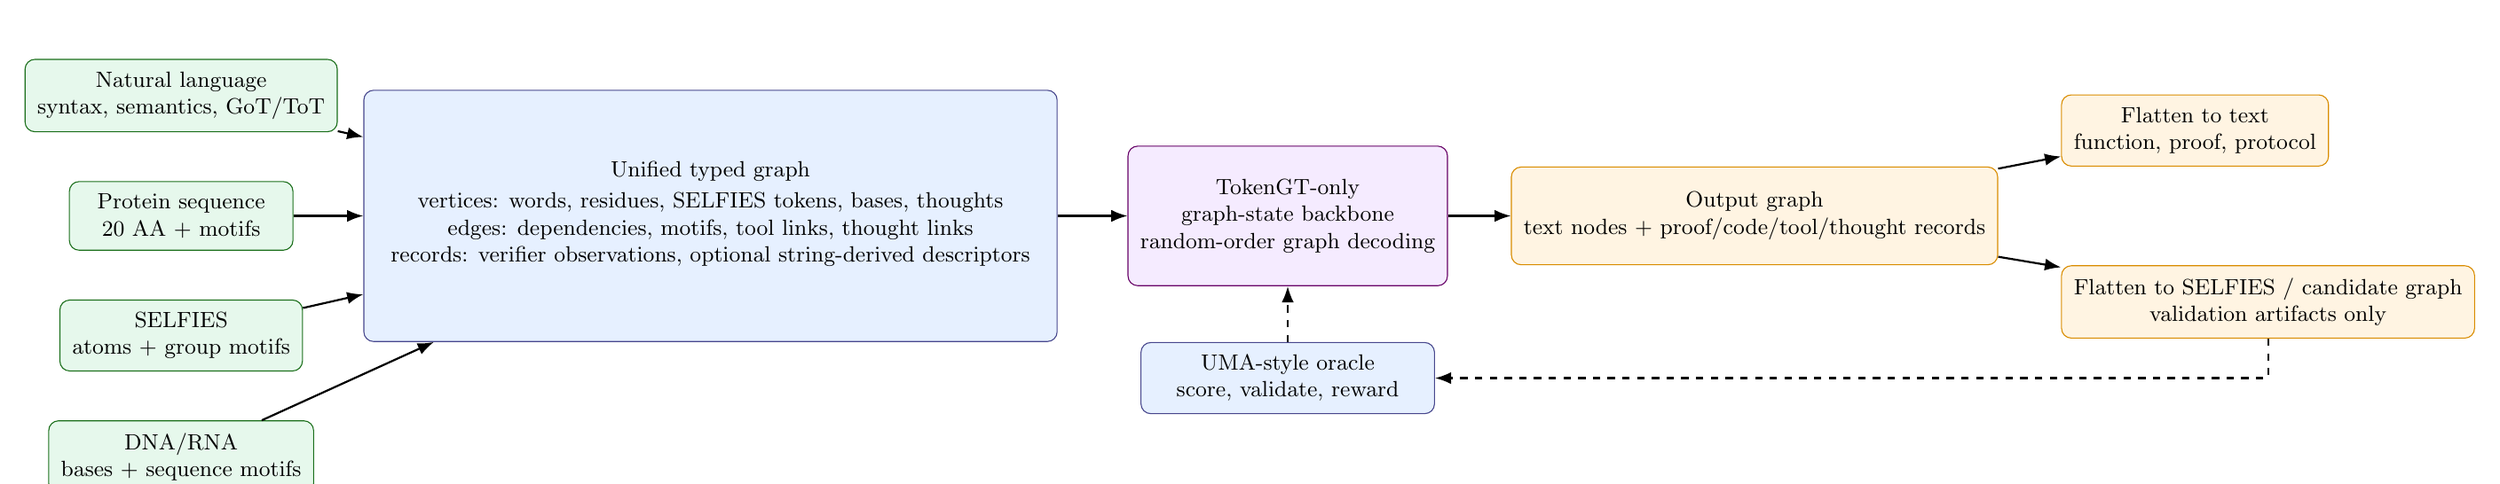
\begin{tikzpicture}[font=\small,node distance=7mm]
\node[gbox,minimum width=3.2cm,minimum height=0.9cm] (lang) {Natural language\\syntax, semantics, GoT/ToT};
\node[gbox,below=of lang,minimum width=3.2cm,minimum height=0.9cm] (prot) {Protein sequence\\20 AA + motifs};
\node[gbox,below=of prot,minimum width=3.2cm,minimum height=0.9cm] (self) {SELFIES\\atoms + group motifs};
\node[gbox,below=of self,minimum width=3.2cm,minimum height=0.9cm] (nuc) {DNA/RNA\\bases + sequence motifs};
\node[box,right=1.0cm of prot,minimum width=4.5cm,minimum height=3.6cm] (graph) {Unified typed graph\\[0.25em]\begin{tabular}{c}vertices: words, residues, SELFIES tokens, bases, thoughts\\edges: dependencies, motifs, tool links, thought links\\records: verifier observations, optional string-derived descriptors\end{tabular}};
\node[pbox,right=1.0cm of graph,minimum width=4.1cm,minimum height=2.0cm] (model) {TokenGT-only\\graph-state backbone\\random-order graph decoding};
\node[obox,right=0.9cm of model,minimum width=4.0cm,minimum height=1.4cm] (outg) {Output graph\\text nodes + proof/code/tool/thought records};
\node[obox,above right=0.0cm and 0.9cm of outg,minimum width=3.8cm] (text) {Flatten to text\\function, proof, protocol};
\node[obox,below right=0.0cm and 0.9cm of outg,minimum width=3.8cm] (pdb) {Flatten to SELFIES / candidate graph\\validation artifacts only};
\node[box,below=0.8cm of model,minimum width=4.2cm] (uma) {UMA-style oracle\\score, validate, reward};
\draw[edge] (lang)--(graph); \draw[edge] (prot)--(graph); \draw[edge] (self)--(graph); \draw[edge] (nuc)--(graph);
\draw[edge] (graph)--(model); \draw[edge] (model)--(outg); \draw[edge] (outg)--(text); \draw[edge] (outg)--(pdb);
\draw[dedge] (pdb)|-(uma); \draw[dedge] (uma)--(model);
\end{tikzpicture}}
\caption{High-level graph-state architecture. Early training uses text, SELFIES/SMILES, protein/DNA/RNA sequences, proof/code/tool traces, and thought graphs. Actual structure files and dynamics trajectories are not training inputs; UMA-style systems are external oracles for validation and reward.}
\label{fig:overview}
\end{figure}

The research hypothesis has four parts. First, graph-token modeling is a natural common interface for language, molecular strings, proteins, nucleic-acid sequences, proof states, code states, and agentic tool traces. Second, random-order graph decoding is a better inductive bias for output graph records than left-to-right decoding whenever the target is a proof dependency graph, a thought graph, a repair graph, or a molecule record set rather than a canonical string. Third, persistent topology and tropical geometry provide useful diagnostics and optional regularizers for latent graph reasoning: topology tracks stable multi-scale shape, while tropical geometry tracks max-like selection and piecewise-linear decision structure. Fourth, an UMA-style oracle can provide validation and reward without changing the architecture or turning structure files into training data. The intended output remains an actual structure-dynamics hypothesis: a typed atom/bond/coordinate/frame graph whose serialization is optional and not required for the present implementation pass. The oracle scores sampled candidate graph states and supplies terminal or process rewards for GFlowNet policies; it is not used here as a direct supervised energy/force/coordinate-label source copied from a structure dataset.

\section{Related systems and what is deliberately excluded}

Modern all-atom structure predictors are powerful but architecturally specialized. AlphaFold 3 uses a diffusion-based architecture for complexes involving proteins, nucleic acids, small molecules, ions, and modified residues \cite{AbramsonAF3_2024}. RoseTTAFold-All-Atom uses residue-level and atomic representations for biomolecular assemblies \cite{KrishnaRFAA2024}. Boltz-1 is an open-source all-atom biomolecular interaction model that reports AlphaFold-3-level accuracy on diverse benchmarks \cite{WohlwendBoltz2025}. Chai-1 is a multimodal molecular structure predictor covering proteins, small molecules, DNA, RNA, and modifications \cite{BoitreaudChai2024,ChaiLab2024}. These systems are essential baselines and inspiration. They are not the architecture proposed here.

Protein language models and protein generation systems are also relevant. ProGen2 scales autoregressive protein language modeling to billions of parameters \cite{NijkampProGen2_2023}. ESM3 jointly reasons over protein sequence, structure, and function with discrete tracks \cite{HayesESM3_2025}. ProstT5 and Foldseek's 3Di alphabet show that structure-derived alphabets can be useful for protein representation and search \cite{HeinzingerProstT5_2023,VanKempenFoldseek2024}. In the current curriculum, such structure-derived alphabets are not used as training targets. They may be reserved for validation, retrieval, or later explicitly approved feature studies. The trainable molecular inputs remain SELFIES/SMILES-style strings and biological sequences.

SELFIES is used because every valid SELFIES string maps to a valid molecular graph under its semantic constraints \cite{KrennSELFIES2020}. Group SELFIES extends this idea with fragment-level tokens \cite{ChengGroupSELFIES2023}. The current training target is therefore molecular string and graph-record reasoning that can propose all-atom, temperature-conditioned structure-dynamics candidates, but the supervision is oracle-guided rather than copied from structure files or MD trajectories. Optional string-derived geometric descriptors, such as non-coordinate RDKit-style 2D descriptors, can be used as features in a later ablation, but this feature is off by default and does not read actual structure files.

The proposal therefore sits between three traditions: graph-token transformers such as TokenGT \cite{KimTokenGT2022}; sequence and molecule language models; and generative graph policies trained with verifiers, tree/graph-of-thought search, and GFlowNets \cite{GatDFM2024,LouSEDD2024,BengioGFlowFoundations2023,VolokhovaConfGFN2024}. Its novelty is the refusal to add a specialist molecular structure architecture during the early curriculum. It asks whether sufficiently rich graph records, random-order decoding, persistent/tropical monitoring, graph-state search, and UMA-oracle rewards can improve scientific reasoning before any direct structure-file training is considered.

\section{The unified multimodal graph object}

\begin{definition}[Multimodal graph-record object]
A training example is a tuple
\[
  X=(G,R,\Gamma),\qquad G=(V,E,\tau_V,\tau_E,a_V,a_E),
\]
where $V$ is a finite set of vertex tokens, $E\subseteq V\times V\times \mathcal R_E$ is a finite set of typed edge records, $\tau_V$ and $\tau_E$ are type maps, $a_V$ and $a_E$ are attribute maps, $R$ is a finite set of non-edge records such as proof states, code states, tool observations, verifier outputs, optional string-derived descriptors, and thought-state records, and $\Gamma$ stores global conditioning variables: modality mask, task, units, graph-state policy, decoding policy, and requested output format.
\end{definition}

The same schema covers every early-training modality. In language, vertices are words, subwords, phrases, proof states, claims, equations, thoughts, tool calls, and observations. Edges are syntax, semantic roles, discourse relations, citations, derivations, graph-of-thought links, and tree-of-thought branches. In proteins, vertices include residues, sequence motifs, domains, and chains. Edges include residue adjacency, motif membership, domain membership, and task constraints. In SELFIES, vertices include SELFIES symbols, SMILES fallback symbols, functional-group motifs, stereochemical markers, and ring/branch records. In DNA/RNA, vertices include bases, sequence motifs, family annotations, and optional non-structure secondary-structure labels. Actual structure files, coordinate frames, and dynamics trajectories are not training inputs in the sequence-first curriculum.

\begin{definition}[Graph record set and serialization renderer]
A graph object $X$ is represented internally as a finite set or multiset of records,
\[
  \mathcal R(X)=\{r_1,\ldots,r_n\},
\]
where each record $r_i$ is a typed token tuple. Early-training examples include \texttt{NODE(residue, chain=A, index=12, aa=W)}, \texttt{NODE(selfies\_token, value=[C])}, \texttt{EDGE(depends\_on, thought3, thought7)}, \texttt{TOOL(result, verifier=lean, status=pass)}, \texttt{ORACLE(score, source=UMA, value=validity\_bin)}, and \texttt{TEXT(role=function, span=...)}. A serializer maps this record set to an ordered list for batching, printing, or file export, but the learned object remains graph-to-graph.
\end{definition}

\subsection{Proteins with residue and sequence-motif vocabularies}

Protein input vocabulary begins with the twenty standard amino acids. It is extended by sequence motifs, domains, organism/taxonomy markers, enzyme annotations, and family labels. Sequence motifs are mined from resources such as InterPro, PROSITE, Pfam-through-InterPro, and reviewed sequence annotations. Structure-derived motifs, torsion patterns, contact patches, coordinate frames, and Foldseek/3Di-like strings are not part of the current training target. They can be kept for evaluation, retrieval, or a later explicitly approved ablation, but the first curriculum is sequence-only.

For future graph rendering or validation, residues can be associated with virtual atom-slot templates. In the current training run, however, these templates are vocabulary and validation scaffolding only. The model is not trained from PDB/mmCIF structures or coordinate labels.

\begin{lemma}[Template-slot sufficiency for fixed residue alphabets]
For any finite residue alphabet with a bounded maximum number of atoms per residue, there exists a finite atom-slot template such that every residue in the alphabet can be represented by an activity mask and atom-identity labels over the template.
\end{lemma}
\begin{proof}
Let $m$ be the maximum number of atoms in any residue in the alphabet after choosing a canonical atom naming scheme. Create $m$ slots. For a residue with $k\leq m$ atoms, map its atoms injectively into the first $k$ compatible slots and mark the remaining $m-k$ slots inactive. Bonds and coordinates are records restricted to active slots. Since the alphabet is finite, $m$ is finite, and the construction represents every residue.\end{proof}

\subsection{SELFIES and SMILES molecules}

SELFIES tokens and SMILES fallback strings are converted to molecular string graphs containing token order, ring/branch markers, charge/stereo markers, and optional functional-group motifs. Motif tokens may include common functional groups, ring systems, fragments from Group SELFIES, pharmacophores, and substructures mined from ChEMBL, ZINC, PubChem, or other non-structure molecule sources. The early curriculum does not train on conformer frames, PDB/HETATM records, SDF coordinate blocks, GEOM conformers, or energy/force labels. Optional string-derived geometric descriptors may be added as features in a controlled ablation, but this path is off by default.

\subsection{DNA and RNA}

DNA and RNA inputs use base tokens $A,C,G,T,U$, ambiguity codes when needed, sequence-family labels, Rfam-family motifs, and non-coordinate secondary-structure annotations when they are available without structure-file supervision. Rfam covariance models and RNAcentral sequence clusters provide sequence and family supervision. NAKB, PDB/NDB-derived structures, and RNA 3D Hub representative sets are evaluation or future-analysis resources, not training inputs in the first curriculum.

\subsection{Mixed complexes and cross-modal prompts}

The model is designed for mixtures: a natural-language task may reference a protein sequence, a ligand SELFIES string, an RNA sequence, a theorem statement, code, or a tool observation. Cross-modal edges attach task constraints to molecular and reasoning subgraphs. Examples include \texttt{ASKS\_ABOUT(prompt, chainA)}, \texttt{TESTED\_AGAINST(ligand, target\_sequence)}, \texttt{VERIFIES(tool, claim)}, and \texttt{FUNCTION\_OF(text, protein)}. Mixed tasks are not a special architecture; they are larger graph states.

\subsection{Input and output graph schemas}

The multimodal task is therefore written as
\[
  X_G \longmapsto Y_G,
\]
not as \(X_G\longmapsto y_1,\ldots,y_T\). The input graph \(X_G\) contains prompt nodes, sequence nodes, SELFIES/SMILES nodes, motif nodes, retrieved context, tool observations, and latent thought nodes. The output graph \(Y_G\) contains one or more of the following: explanatory text nodes connected by discourse and citation edges; proof or code nodes connected by dependency edges; graph-of-thought/tree-of-thought nodes; verifier records; UMA-oracle reward records; SELFIES renderings; and repair/action records. Structure serializers such as SDF/mmCIF/PDB are validation artifacts only under the current curriculum, not supervised training targets.

\begin{table}[H]
\centering
\caption{Primary graph-to-graph interpretation of multimodal outputs.}
\scriptsize
\setlength{\tabcolsep}{3pt}
\begin{tabular}{p{0.19\linewidth}p{0.39\linewidth}p{0.27\linewidth}}
\toprule
Requested surface output & Primary decoded output graph & Optional flattening/rendering \\
\midrule
Function description & Claim nodes, evidence nodes, ontology nodes, uncertainty edges, citation/support edges & Natural-language paragraph or report \\
Sequence-backed biomolecular reasoning & Residue/base nodes, SELFIES/SMILES nodes, motifs, assay/function nodes, verifier edges & Natural-language answer, SELFIES string, graph record report \\
Oracle-scored candidate graph & Candidate nodes, validity nodes, UMA reward records, repair/action edges & Ranked candidate list or tool trace \\
Proof or code & Lemma/function nodes, dependency edges, tactic/API-call nodes, verifier-result nodes & Lean script or source file \\
Agentic plan & Thought nodes, branch edges, tool-call nodes, observation nodes, reward/verifier nodes & Linear transcript or execution log \\
\bottomrule
\end{tabular}
\end{table}


\section{Vocabulary augmentation}

\begingroup\scriptsize\setlength{\tabcolsep}{2pt}
\begin{longtable}{p{0.13\linewidth}p{0.28\linewidth}p{0.33\linewidth}}
\caption{Core vocabulary families. The list is extensible but architecture-neutral: new terms are tokens and records, not new modules.}\\
\toprule
Family & Tokens & Purpose \\
\midrule
\endhead
Text and reasoning & subwords, words, phrases, syntax edges, semantic-role edges, theorem/proof states, tool-call records, GoT/ToT edges & General language, mathematical reasoning, function descriptions, and agentic tool traces. \\
Protein residues & 20 standard amino acids, chain markers, residue indices, sequence-window tags & Protein sequence modeling and FASTA-grounded reasoning without structure-file inputs. \\
Protein motifs & PROSITE/InterPro motifs, CATH/3Di-derived sequence-motif vocabulary tokens, domain and family annotations & Compression, inductive bias, and function annotation. Structure-derived sequence motifs are allowed only as frozen sequence tokens, not as row-level coordinates or contact labels. \\
SELFIES chemistry & standard SELFIES tokens, ring/branch markers, charge/stereo tokens, Group-SELFIES-like fragments, pharmacophore motifs & Robust molecular graph input and fragment-level compression. \\
DNA/RNA & bases, ambiguity symbols, Rfam-family tokens, covariance-family tokens, sequence-derived loop/helix motif tokens, modified-base sequence tags & Nucleic-acid sequence reasoning and annotation without direct 3D structure supervision. \\
Optional geometry features & string-derived descriptors, ring counts, molecular weight, TPSA, logP, rotatable-bond count & Off by default; no structure-file training. \\
Oracle/verifier & UMA validity/reward bins, temperature-conditioned score bins, tool status, repair hints, verifier confidence & External scoring and GFlowNet rewards, not direct energy/force-label training. \\
Attention/coupling/motion & Stage-specific 64-bin attention-coupling records, UMA-influence records, token-coupling records, token-motion and trajectory-proxy records & Routing and graph-state evolution supervision for the UMA sequence-to-structure-dynamics proxy stage only. \\
\bottomrule

\end{longtable}\endgroup

\subsection{Mandatory bond-type and molecular-edge vocabulary}

Bond type is a first-class edge token for molecular graph reasoning. A molecular edge without bond type is insufficient for valence, aromaticity, stereochemistry, protonation, conjugation, and downstream validation. \UGM{} therefore represents a covalent or noncovalent edge hypothesis as a typed record
\[
  e=(u,v,\mathrm{edge\_class},\mathrm{bond\_type},\mathrm{stereo},\mathrm{aromatic},\mathrm{order},\mathrm{confidence}),
\]
where \(\mathrm{bond\_type}\) ranges over at least
\[
\begin{aligned}
\mathrm{bond\_type}\in\{&\text{none},\text{single},\text{double},\text{triple},\text{aromatic},\text{amide},\text{peptide},\\
&\text{phosphodiester},\text{glycosidic},\text{disulfide},\text{dative},\text{coordinate},\\
&\text{ionic},\text{hydrogen},\text{base-pair},\text{stacking}\}.
\end{aligned}
\]
SELFIES-derived molecules require single, double, triple, aromatic, ring-closure, branch, stereochemical, formal-charge, and valence records. Proteins and nucleic acids may use peptide, disulfide, hydrogen-bond, salt-bridge, phosphodiester, glycosidic, Watson-Crick, wobble, Hoogsteen, and stacking records as graph hypotheses or validation labels when they are available without structure-file supervision. Bond-type tokens are used as input features and decoded graph records; validators parse them before UMA-oracle reward or tool-based repair is trusted.

\begin{lstlisting}[caption={Bond-type-aware edge records.}]
REC EDGE src=LIG:C7 dst=LIG:O8 edge=COVALENT bond_type=DOUBLE order=2
REC EDGE src=A:42:SG dst=B:91:SG edge=COVALENT bond_type=DISULFIDE order=1
REC EDGE src=RNA:12:G dst=RNA:31:C edge=BASE_PAIR bond_type=WATSON_CRICK orientation=CIS
REC EDGE src=ZN:1 dst=HIS:57:NE2 edge=COORDINATE bond_type=DATIVE charge_context=+2
\end{lstlisting}

\subsection{Motif construction without leakage}

Motifs must be mined only from training splits. For proteins, cluster sequence windows, family annotations, and domain annotations. For small molecules, mine SELFIES/SMILES fragments, frequent non-coordinate subgraphs, and functional groups. For RNA, mine sequence-family and covariance-model motifs. For language and reasoning, mine parse motifs, proof motifs, CoT motifs, GoT motifs, and ToT branch motifs. Row-local structure-derived motifs, contact neighborhoods, torsion patterns, coordinate-derived 3D motifs, and structure files are excluded from the current train split and can only be used for validation or a later explicitly approved ablation. A separate safe case is allowed: a frozen vocabulary of \emph{sequence motifs derived from structure-motif catalogs}, such as CATH/3Di-inspired sequence-window names, may be represented by tokens such as \texttt{SEQ\_MOTIF\_FROM\_STRUCTURE:*} only when the training row contains no coordinates, atom records, contact labels, distance maps, PDB/mmCIF/SDF files, or trajectory fields. Motif vocabularies are frozen before validation and test data are processed.

\begin{lstlisting}[caption={Leakage-safe motif mining.}]
def mine_motifs(train_examples, modality, min_support, max_size):
    candidates = Counter()
    for x in train_examples:
        g = parse_to_graph(x, modality)
        for subgraph in enumerate_connected_subgraphs(g, max_size=max_size):
            code = canonicalize(subgraph, ignore_coordinates=True)
            if passes_domain_filters(code, modality):
                candidates[code] += 1
    motifs = [c for c,n in candidates.items() if n >= min_support]
    motifs = remove_near_duplicates(motifs)
    return freeze_vocabulary(rank_by_mdl_gain(motifs))
\end{lstlisting}

\subsection{Vertex-to-edge and edge-to-vertex weighting without changing architecture}

The requested attention-weighting paradigm is implemented as data and loss, not as a new attention operator. For a graph with attention matrices $A^{(\ell,h)}$, define a sparse coupling prior $P$ over token pairs. $P_{ve}$ is high when vertex $v$ is incident to edge token $e$; $P_{ev}$ is high when edge $e$ should return information to vertex $v$; $P_{thought}$ is high for GoT/ToT/CoT dependency edges; $P_{tool}$ is high for tool-call/result pairs; and $P_{oracle}$ is high for UMA-oracle score and candidate records. The 64-way records below are emitted only in the UMA sequence-to-structure-dynamics proxy stage. Ordinary SELFIES/FASTA/RNA/DNA reconstruction and function-description rows may include temperature and function-description graph nodes, but they do not create these fine-bin targets unless an oracle/proxy stage flag or structure-dynamics task is active. In the active UMA proxy stage, the implementation exposes these priors as binned graph records,
\[
\texttt{ATTN\_BIN:route:b00\ldots b63},\qquad
\texttt{TOKEN\_COUPLING:uma:channel:b00\ldots b63},
\]
with companion records
\[
\texttt{UMA\_INFLUENCE:uma:channel:b00\ldots b63},\qquad
\texttt{TOKEN\_MOTION:uma:action:b00\ldots b63},\qquad
\texttt{UMA\_TRAJ\_BIN:action:b00\ldots b63}.
\]
The 64-way ordinal binning is intentionally closer to modern structure-prediction practice than a four-level heuristic, but it is not a global objective across all stages. AlphaFold 3, for example, can emit a token-pair distogram tensor of shape \((n,n,64)\) and also exposes single-token and pair embeddings \cite{AbramsonAF3_2024,AlphaFold3Output2026}. UGM does not copy AF3's architecture or train on AF3 targets. It adopts the same engineering lesson for the UMA proxy stage: pairwise geometric uncertainty should be represented as a distribution over many bins rather than as one coarse label. Routes include \texttt{sequence\_to\_motif}, \texttt{motif\_to\_oracle}, \texttt{temperature\_to\_oracle}, and \texttt{sequence\_to\_motion}. UMA feedback therefore influences token coupling, token motion, and candidate trajectory records: low-temperature oracle scoring sharpens bins toward refinement and stabilization, while high-temperature oracle scoring shifts mass toward exploration and diversification. Add
\[
  \mathcal L_{\mathrm{attn}} = \sum_{\ell,h}\lambda_{\ell,h}\,\mathrm{KL}\big(P\,\|\,A^{(\ell,h)}+\epsilon\big).
\]
This encourages vertex-to-edge and edge-to-vertex routing but leaves the TokenGT block unchanged. When internal attention matrices are unavailable or too expensive to regularize directly, the binned records are still trained by random-order likelihood and by GFlowNet reward. The same bins also determine decoding-order proposals: high-priority sequence, motif, attention-bin, coupling, UMA-influence, motion, verifier, and UMA-oracle records are decoded before lower-priority explanation records. In the first curriculum these bins are learned from SELFIES and FASTA-style sequence inputs plus oracle-scored graph-state traces; they are not learned from structure files.

\subsection{Embedding-distribution geometry and Jensen-Shannon monitoring}

The model may also use geometric information already present in its hidden embeddings. For hidden token states \(h_i\in\mathbb R^d\), define a distribution
\[
  p_i=\mathrm{softmax}(h_i/\tau_h).
\]
For two tokens \(i,j\), the Jensen-Shannon divergence is
\[
  \mathrm{JS}(p_i,p_j)=\frac12\KL(p_i\|m_{ij})+\frac12\KL(p_j\|m_{ij}),
  \qquad m_{ij}=\frac12(p_i+p_j),
\]
and the bounded distance \(d_{\rm JS}(i,j)=\sqrt{\mathrm{JS}(p_i,p_j)}\) gives a complementary geometry to Euclidean embedding distance. The monitor therefore computes both Euclidean distograms and JS-distance distograms over hidden graph-token states. Optional regularization can discourage collapse in either geometry:
\[
  \mathcal L_{\rm JS}=\left[\delta-\E_{i<j}d_{\rm JS}(i,j)\right]_+^2.
\]
This is a training-guidance option for ablation, not an architectural change. The first experiment should compare baseline, topology-only, tropical-only, JS/topology, and combined variants under equal compute and report quality, diversity, wall-clock cost, and oracle-score efficiency.

\subsection{Evolving attention maps as fold-contact fields}

The mechanism by which sequence-only training can still produce structure-dynamics candidates is that attention couplings are treated as an evolving contact field. Let \(A_t^{\ell,h}\in[0,1]^{n\times n}\) be an attention map at graph-state step \(t\), layer \(\ell\), and head \(h\). A symmetrized attention-contact proxy is
\[
  C_t^A(i,j)=\sum_{\ell,h}w_{\ell h}\frac12\left(A_t^{\ell,h}(i,j)+A_t^{\ell,h}(j,i)\right).
\]
Embedding geometry and probability geometry add two compatible fields,
\[
  C_t^E(i,j)=\exp\left(-\frac{\|z_i^t-z_j^t\|_2^2}{\sigma_E^2}\right),
  \qquad
  C_t^{JS}(i,j)=\exp\left(-\frac{d_{JS}(p_i^t,p_j^t)^2}{\sigma_{JS}^2}\right),
\]
and the working fold-contact field is
\[
  C_t(i,j)=\alpha_A C_t^A(i,j)+\alpha_E C_t^E(i,j)+\alpha_{JS}C_t^{JS}(i,j).
\]
Persistent high mass in \(C_t(i,j)\), especially for sequence-distant pairs, is interpreted as a latent contact hypothesis. The motion \(\Delta C_t=C_{t+1}-C_t\) is a folding-like graph-state motion: contacts form, dissolve, or sharpen as the latent state evolves. For proteins these indices may denote residue or motif tokens; for SELFIES they may denote atom-slot or functional-group tokens; for RNA and DNA they may denote base, loop, or pairing-hypothesis tokens.

The coordinate and frame decoder should emit candidate atom, bond, coordinate, and frame records whose rendered distances agree with this contact field. For generated coordinates \(x_i^f\), define
\[
  \widehat C_f(i,j)=\sigma\left(\frac{r_c-\|x_i^f-x_j^f\|_2}{s_c}\right).
\]
A self-consistency term
\[
  \mathcal L_{\mathrm{contact\mbox{-}coord}}=
  \sum_{f,i<j}\left(C_t(i,j)-\widehat C_f(i,j)\right)^2
\]
does not use a ground-truth structure file. It only ties the model's own attention/embedding/JS contact hypothesis to the generated coordinate/frame graph it emits. UMA then scores the candidate graph at the chosen continuous temperature, with optional serialization only when a downstream renderer is enabled. GFlowNet trajectory balance reinforces graph-state trajectories whose evolving contact maps and generated coordinates receive high UMA reward. Thus attention maps can, in principle, evolve to encode actual folding contacts without supervised structure-file training; the empirical question is how much accuracy this reward-only route can buy under the available compute.

\section{Random-order autoregressive graph decoding}

Left-to-right decoding is appropriate for many rendered text strings, but neither an output proof graph nor a molecular string graph is a privileged string. A proof, code repair, tool trace, SELFIES record set, or graph-of-thought state can be revealed in many valid orders. Random-order decoding trains the model to complete arbitrary missing records of an output graph conditioned on an input graph.

\begin{definition}[Random-order likelihood]
Let $X_G$ be the input graph and let $\mathcal R(Y_G)=\{r_1,\ldots,r_n\}$ be the output graph-record set. For a permutation $\pi\in S_n$, define
\[
  p_\theta(Y_G\mid X_G,\pi,\Gamma)=\prod_{t=1}^n p_\theta(r_{\pi_t}\mid X_G,r_{\pi_{<t}},\Gamma,\pi_{\le t}).
\]
The symmetrized likelihood is
\[
  p_\theta^{\mathrm{sym}}(Y_G\mid X_G,\Gamma)=\frac{1}{n!}\sum_{\pi\in S_n}p_\theta(Y_G\mid X_G,\pi,\Gamma).
\]
Training samples permutations or structured order policies and maximizes the corresponding Monte Carlo lower bound.
\end{definition}

\begin{proposition}[Order-sampled training lower bounds the symmetrized likelihood]
For any distribution $q(\pi\mid X_G,Y_G)$ with full support,
\[
\log p_\theta^{\mathrm{sym}}(Y_G\mid X_G,\Gamma)\geq
\E_{\pi\sim q}\left[\log p_\theta(Y_G\mid X_G,\pi,\Gamma)-\log(n!q(\pi\mid X_G,Y_G))\right].
\]
\end{proposition}
\begin{proof}
Write the symmetrized graph-to-graph likelihood as an expectation under $q$ and apply Jensen's inequality to the logarithm.\end{proof}

\begin{figure}[H]
\centering
\resizebox{0.92\linewidth}{!}{%
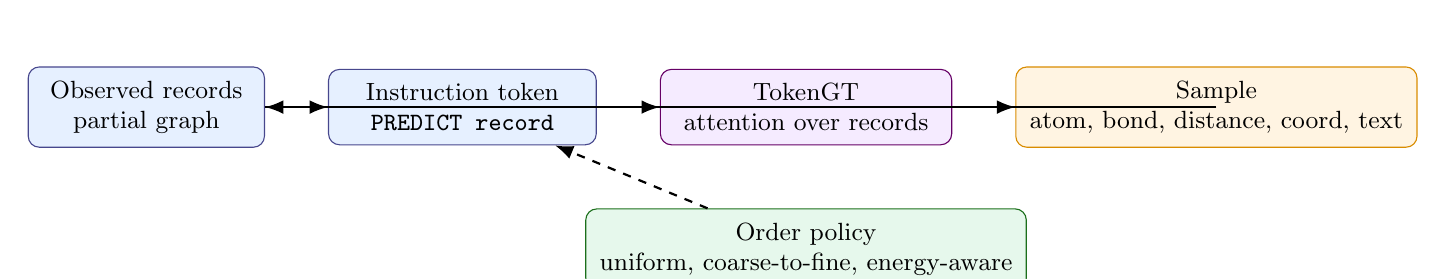
\begin{tikzpicture}[font=\small,node distance=8mm]
\node[box,minimum width=3.0cm] (obs) {Observed records\\partial graph};
\node[box,right=of obs,minimum width=3.4cm] (instr) {Instruction token\\\texttt{PREDICT record}};
\node[pbox,right=of instr,minimum width=3.7cm] (model) {TokenGT\\attention over records};
\node[obox,right=of model,minimum width=3.4cm] (sample) {Sample\\atom, bond, distance, coord, text};
\node[gbox,below=of model,minimum width=3.7cm] (policy) {Order policy\\uniform, coarse-to-fine, energy-aware};
\draw[edge] (obs)--(instr); \draw[edge] (instr)--(model); \draw[edge] (model)--(sample); \draw[edge] (sample)|-(obs); \draw[dedge] (policy)--(instr);
\end{tikzpicture}}
\caption{Random-order graph-to-graph autoregression. The next output record may be a SELFIES token, residue token, motif token, claim node, thought node, tool result, verifier result, UMA-oracle score, or repair action, always conditioned on the input graph and the partial output graph.}
\label{fig:random}
\end{figure}

\subsection{Three generation views}

Random-order autoregression, masked discrete diffusion, and discrete flow matching are treated as three parameterizations of conditional graph-to-graph completion. In the random-order view, a policy chooses the next missing record and samples it. In the masked diffusion view, the graph starts with many mask records and is iteratively denoised. In the discrete flow-matching view, one learns a categorical transport field from a base masked distribution to the data distribution. These views can share the same TokenGT conditional distribution and differ only in schedule, objective, and sampler.

\begin{lstlisting}[caption={Random-order graph training step.}]
def training_step(example):
    records = graphify_sequence_or_reasoning_example(example)
    order = sample_order(records, policy_mix=[uniform, verifier_enabling, thought_graph])
    prefix, targets = [], []
    loss = 0
    for r in order:
        instr = make_instruction(r.type, r.scope)
        logits = model(prefix + [instr], conditioning=example.context)
        loss += cross_entropy(logits, r)
        prefix.append(r)
    loss += sequence_validity_losses(prefix) + graph_state_losses(prefix)
    loss += oracle_reward_modeling_loss(prefix) + attention_coupling_loss(model.attn)
    return loss
\end{lstlisting}

\section{Temperature-conditioned UMA-oracle curriculum}

The model receives temperature as a continuous conditioning variable \(T\in[300,400]\,\mathrm K\), or a nearby bounded interval chosen by the experiment. The discrete high-to-low ladder \(\{400,375,350,325,300\}\,\mathrm K\) is only a curriculum scaffold and evaluation grid. The actual graph record stores both a rounded anchor token, for vocabulary stability, and continuous scalar features such as \(T\), \((T-300)/100\), and \(300/T\). The ladder teaches the graph-state policy that candidate choices, verifier confidence, and UMA-oracle rewards depend smoothly on the requested temperature. It does not train on MD trajectories, PDB frames, force fields, or coordinate labels.

For a candidate molecular graph state \(Y_G\), an UMA-style oracle can return a binned validity or reward signal
\[
  R_T(Y_G)=Q_{\rm validity}(Y_G)\,Q_{\rm task}(Y_G)\,\exp\{-\beta_T \widehat E_{\rm oracle}(Y_G)\},
\]
where \(\beta_T=(k_BT)^{-1}\) and \(\widehat E_{\rm oracle}\) is an oracle-provided score for a candidate graph, not a supervised training label extracted from an actual structure file. UMA is called with the same continuous \(T\) that is encoded in the graph state, so temperature changes the oracle score rather than merely labeling the example. The model conditions on \(T\) and learns which graph-state actions tend to receive higher oracle reward at different temperatures.

\begin{lstlisting}[caption={Continuous-temperature UMA-oracle graph-state curriculum.}]
def sample_temperature_schedule(anchors=[400,375,350,325,300],
                                jitter_k=6.0,
                                bounds=(300.0, 400.0)):
    for anchor in anchors:
        yield clamp(anchor + uniform(-jitter_k, jitter_k), *bounds)

def build_temperature_conditioned_trace(input_graph):
    traces = []
    for T in sample_temperature_schedule():
        G = input_graph.with_continuous_temperature(T)
        for step in range(max_graph_state_steps):
            action = policy.sample(G)
            G_next = apply_graph_state_action(G, action)
            oracle = UMA_oracle_score(G_next, temperature=T)
            traces.append((G, action, G_next, T, oracle.reward_bin))
            G = repair_or_continue(G_next, oracle)
    return traces
\end{lstlisting}

This is the role of the high-to-low temperature annealing ladder in the current paper. It creates a curriculum of \emph{continuous conditioning features and oracle-scored graph-state decisions}. It should improve whether the model interprets \(T=397.5\,\mathrm K\) differently from \(T=302.5\,\mathrm K\), and whether its GoT/ToT/GFlowNet policy searches broadly at high temperature and more selectively at low temperature. It is not an instruction to train on actual structure or dynamics files.

\subsection{GFlowNet objective}

Let a trajectory $\tau$ be a sequence of graph-state actions ending in a candidate record graph \(Y_G\). In the sequence-first curriculum, \(Y_G\) may contain SELFIES/SMILES records, protein or nucleotide sequence annotations, claim and evidence nodes, tool-call records, thought nodes, oracle-feedback records, and generated atom, bond, coordinate, frame, and optional serializer records. These generated structure-dynamics records are sampled candidate hypotheses, not supervised labels copied from actual structure files, MD frames, or force datasets. Define a temperature-conditioned oracle reward
\[
R_T(Y_G)=Q_{\rm validity}(Y_G)\,Q_{\rm task}(Y_G)\,
\exp\{-\beta_T \widehat E_{\mathrm{UMA}}(Y_G)\},
\]
where \(\widehat E_{\mathrm{UMA}}\) is a scalar score returned by the external oracle for the candidate graph at the requested continuous temperature. Trajectory balance trains forward and backward policies so terminal graph states are sampled proportional to this reward, while the model learns the \emph{conditioning effect} of \(T\) through the continuous temperature feature and oracle-feedback records.

\begin{theorem}[Trajectory-balance optimum]
Assume a finite acyclic construction graph, positive terminal rewards, and expressive forward/backward policies. At a global optimum of the trajectory-balance objective, the terminal distribution of the forward policy is proportional to \(R_T(Y_G)\).
\end{theorem}
\begin{proof}
The standard trajectory-balance equations enforce equality between the total flow into a terminal object and its reward. Summing over all trajectories leading to a terminal graph state gives terminal flow proportional to \(R_T\). Normalizing flows gives the forward terminal distribution.\end{proof}

\section{Datasets and curation}

The dataset program has five layers: language and reasoning traces; biological sequence corpora; SELFIES/SMILES molecule corpora; oracle-scored graph-state traces; and evaluation-only structure or dynamics resources. The training split intentionally excludes actual structure files, coordinate trajectories, force fields, and direct physics labels. All splits must control leakage. Protein splits should be clustered by sequence identity and temporal release. Small molecules should be split by scaffold, InChIKey block, and sometimes by time. RNA should be split by family and motif. Motif vocabularies are mined only from training data.

The expanded corpus and split program in Section~\ref{sec:additional-datasets} should be treated as the primary replication specification. The table below is a modality-level summary for the sequence-first multimodal component; the complete implementation uses the entity-aware split registry of Section~\ref{sec:entity-aware-splits}. Resources with actual structures or trajectories are marked evaluation-only unless a later, explicit phase enables them.

{\scriptsize
\setlength{\tabcolsep}{2pt}
\begin{longtable}{p{0.16\linewidth}p{0.22\linewidth}p{0.34\linewidth}p{0.06\linewidth}}
\caption{Primary datasets and construction sources.}\\
\toprule
Modality & Resource & Use & Ref. \\
\midrule
\endhead
Language & FineWeb, Dolma, OpenWebMath, The Stack, tool logs, Lean/math corpora & Instruction, math, code, CoT/ToT/GoT traces, explanation, verifier transcripts. & Refs. \\
Protein sequence & UniProt, UniRef, UniParc, metagenomic resources when license permits & Protein sequence modeling, family clustering, function annotation, sequence motif mining. & Refs. \\
Protein annotations & InterPro, PROSITE, CATH-Gene3D sequence annotations, GO, EC, UniProt fields & Domain/function tokens, motif labels, claim/evidence supervision. & Refs. \\
SELFIES/SMILES molecules & PubChem, ChEMBL, ZINC, MoleculeNet, BindingDB, PubChemQC identifiers/properties & SELFIES/SMILES reconstruction, scaffold-aware splits, property and assay reasoning. & Refs. \\
DNA/RNA sequence & GenBank, RefSeq, Ensembl, RNAcentral, Rfam & Nucleotide sequence pretraining, family labels, covariance/secondary-structure annotations when not derived from structure files. & Refs. \\
Oracle graph traces & UMA-style oracle calls, validators, RDKit string validators, proof/code tools & Temperature-conditioned reward bins, validity records, repair traces, GFlowNet terminal rewards. & Refs. \\
Evaluation-only structures & RCSB PDB, wwPDB, AlphaFold DB, NAKB, RNA 3D Hub, GEOM, SPICE, ATLAS, mdCATH & Structure-side validation, leakage audits, and future-phase comparison only; excluded from first training curriculum. & Refs. \\
\bottomrule
\end{longtable}}

\subsection{Graphification pipeline}

\begin{lstlisting}[caption={End-to-end data graphification.}]
def graphify_example(raw):
    modality = detect_modality(raw)
    if modality == "language":
        g = parse_language_to_graph(raw.text)
    elif modality == "protein":
        g = residue_graph(raw.sequence)
        g.add(motif_matches(raw.sequence, protein_motif_vocab))
    elif modality == "selfies":
        g = molecular_string_graph(raw.selfies_or_smiles)
        g.add(fragment_motifs(raw.selfies_or_smiles, selfies_motif_vocab))
        if geometric_features_enabled:
            g.add(string_derived_2d_descriptors(raw.selfies_or_smiles))
    elif modality in ["DNA", "RNA"]:
        g = nucleotide_graph(raw.sequence)
        g.add(nucleic_motifs(raw.sequence))
    if raw.temperature: g.add(global_token(f"TEMP_{raw.temperature}K"))
    g = remove_actual_structure_fields(g)
    records = canonicalize_to_record_set(g)
    return records
\end{lstlisting}

\subsection{Function-description and medicine-design data}

Text output should include biochemical function descriptions, but those descriptions must be grounded. Construct pairs from SFM/NatureLM-style sequence science records, UniGenX sequence/function metadata after structure sanitization, ProTrek-style protein sequence/function pairs, UniProt function fields, Gene Ontology annotations, enzyme commission numbers, InterPro domains, ChEMBL target annotations, BindingDB assay metadata, Open Targets evidence, and curated literature abstracts. The curation rule is conservative: a generated function target is included only when the graph contains explicit supporting annotations. For ProTrek-style data, the first-run slice keeps protein sequences and natural-language function descriptions, converts contrastive positives and hard negatives into graph pairs, and excludes structure tracks except as evaluation-only retrieval audits. For medicine-design prompts in the first curriculum, use SELFIES/SMILES strings, sequence records, assay labels, target annotations, function descriptions, and tool/verifier observations to build explanatory tasks such as: identify scaffold families, explain sequence-function evidence, propose candidate edits for an oracle to score, or describe why a candidate graph violates a string-level chemical or biological constraint. Structure-derived binding-pocket, conformer-refinement, and coordinate-repair tasks are evaluation-only or future-phase tasks, not first-run training data.

\section{Training objectives}

The full objective is a weighted sum:
\[
\mathcal L=\mathcal L_{\mathrm{ROA}}+
\lambda_S\mathcal L_{\mathrm{seq}}+
\lambda_R\mathcal L_{\mathrm{reason}}+
\lambda_V\mathcal L_{\mathrm{verify}}+
\lambda_O\mathcal L_{\mathrm{oracle}}+
\lambda_G\mathcal L_{\mathrm{GFN}}+
\lambda_A\mathcal L_{\mathrm{attn}}+
\lambda_I\mathcal L_{\mathrm{id}}+
\lambda_T\mathcal L_{\mathrm{top/trop}}.
\]
Here $\mathcal L_{\mathrm{ROA}}$ is random-order autoregressive cross entropy over output graph records conditioned on input graph records. $\mathcal L_{\mathrm{seq}}$ reconstructs SELFIES/SMILES, protein, DNA, RNA, and text/proof/code sequences as graph records. $\mathcal L_{\mathrm{reason}}$ supervises CoT, ToT, and GoT state transitions. $\mathcal L_{\mathrm{verify}}$ predicts verifier pass/fail and repair records. $\mathcal L_{\mathrm{oracle}}$ predicts binned UMA-oracle feedback records produced for sampled candidate graph states at continuous temperature conditions with rounded anchor/bin tokens; it is not an energy/force regression loss against a structure-file dataset. $\mathcal L_{\mathrm{GFN}}$ is trajectory-balance or flow-matching loss over graph-state trajectories. $\mathcal L_{\mathrm{attn}}$ supervises vertex-edge, thought-tool, sequence-motif, and oracle-feedback routing through binned coupling records. $\mathcal L_{\mathrm{id}}$ checks orthogonal vertex/edge identifier routing. $\mathcal L_{\mathrm{top/trop}}$ regularizes persistent and tropical summaries when the ablation enables those terms. The sequence-to-structure-dynamics target is therefore a generated candidate graph state,
\[
  X_{\rm SELFIES/FASTA},T \longmapsto
  \{\texttt{SEQ\_STRUCT\_DYN\_PROXY},\texttt{ATTN\_BIN},\texttt{TOKEN\_COUPLING},\texttt{UMA\_INFLUENCE},\texttt{TOKEN\_MOTION},\texttt{UMA\_TRAJ\_BIN},\texttt{ATOM},\texttt{BOND},\texttt{COORD},\texttt{FRAME}\},
\]
which is scored by UMA and validators. It is not supervised by copied coordinates, force labels, PDB/mmCIF/SDF rows, or MD frames during the first run; generated coordinate and frame records are still part of the model's sampled output behavior, while PDB serialization can remain optional.

\subsection{Persistent topology and tropical geometry}

For a point cloud of latent embeddings, thought-node states, graph-token states, or sampled candidate-record embeddings, compute persistent summaries such as connected components, loops, and multi-scale cluster lifetimes. Use these as diagnostics and optional losses: successful reasoning should preserve useful non-linear thought topology, avoid premature collapse, and maintain stable morphology-aware and sequence-aware components when they matter. Tropical geometry enters through max-plus selection. In low-temperature attention,
\[
\mathrm{softmax}(s/\tau)\rightarrow \arg\max_i s_i\quad\mathrm{as}\quad\tau\rightarrow0,
\]
and ReLU networks are piecewise affine over polyhedral regions. Tropical diagnostics track sharp region changes during graph decisions: selecting a motif, thought branch, tool call, verifier repair, SELFIES edit, or oracle-query action. A tropical regularizer can penalize unstable max selections under small input perturbations unless the verifier or oracle reward strongly supports a sharp transition.

\section{Sampling algorithms}

\subsection{Random-order autoregressive sampling}

\begin{lstlisting}[caption={Continuous-temperature random-order sampler.}]
def sample_ugm(context, anchors=[400,375,350,325,300]):
    records = initialize_records(context)
    graph_state_trace = []
    for T in sample_temperature_schedule(anchors):
        records.add(continuous_temperature_record(T))
        while not complete_reasoning_state(records, T):
            scope = choose_missing_scope(records, policy="oracle_aware")
            instr = make_predict_instruction(scope)
            r = sample_model(records + [instr], top_p=0.95, temperature=decode_temp(T))
            records.add(r)
            if should_query_oracle(records):
                records.add(UMA_feedback_records(records, temperature=T))
        graph_state_trace.append(snapshot_graph_state(records, T))
    return render_answer_or_candidate_records(graph_state_trace)
\end{lstlisting}

\subsection{Masked discrete diffusion-style sampling}

Initialize target reasoning, sequence, tool, and oracle-feedback records as \texttt{MASK}. At each step, the model predicts a subset of masked records conditioned on the visible graph, then remasks or refines low-confidence records. The schedule can be temperature-aware: high-temperature conditions encourage broader candidate exploration and more diverse graph-state branches; low-temperature conditions encourage stricter verifier/oracle filtering and shorter repair paths.

\subsection{Discrete flow-matching-style sampling}

Treat graph records as categorical states and train a time-indexed model to map a base masked distribution toward the data distribution. The flow predicts replacement rates for record types. For sequence-first molecular graphs, a useful schedule first creates modality and task records, then SELFIES/SMILES or residue/base sequence records, then motif and annotation records, then thought/tool/oracle records. Unlike standard left-to-right decoding, flow steps can update many records in parallel.

\subsection{GFlowNet sampling}

GFlowNet sampling is used when diversity matters. Instead of seeking one best answer or molecule string, the model samples multiple candidate graph states with probability proportional to verifier and UMA-oracle reward. For temperature-conditioned molecular reasoning, the reward is a Boltzmann-like scalar returned by the oracle for a candidate graph at the requested temperature, corrected by validity and task constraints. The output may include generated atom, bond, coordinate, and frame records together with explanations; what is excluded in the first run is supervised coordinate or trajectory copying from structure/dynamics datasets.


\section{Theoretical implications}

\begin{theorem}[Finite graph representability]
For any finite collection of language, protein-sequence, SELFIES/SMILES, DNA, RNA, tool-trace, oracle-feedback, and reasoning examples with bounded size and finite categorical fields, there exists a finite graph-record vocabulary extension that represents every input example and every output example exactly.
\end{theorem}
\begin{proof}
Each example contains finitely many discrete labels and, when needed, finitely many binned verifier or oracle fields. Add a token or tuple schema for each required label, relation, and bin. The union over a finite dataset is finite. Encoding each object as node, edge, hyperedge, attribute, tool, verifier, oracle, thought, and serializer records gives exact representation at the chosen precision.
\end{proof}

\begin{theorem}[Multimodal TokenGT graph-to-graph representability]
Fix bounded graph-record classes for the four input modalities considered here: natural language/reasoning graphs, protein-sequence graphs, SELFIES/SMILES molecular-string graphs, and DNA/RNA sequence graphs. Fix a bounded output class containing text graphs, proof/code graphs, thought graphs, tool/verifier graphs, oracle-feedback graphs, and candidate molecule-sequence graphs. Every deterministic target map from these input classes to the output class can be represented as a map between finite record sets; if the map is continuous in the record-feature topology, it is uniformly approximable by a TokenGT-style graph-to-graph transformer in the sense of the universality theorem above.
\end{theorem}
\begin{proof}
Finite-precision bounded graphs can be embedded into fixed padded input and output tensors by record-injective TokenGT encoders. The deterministic target is therefore a finite-dimensional function between compact encoded subsets. If it is merely a finite lookup map on a finite dataset, exact memorization is possible by a sufficiently large continuous approximator with separated neighborhoods. If it is continuous on the compact graph-record class, the TokenGT graph-to-graph universality theorem gives uniform approximation. The modalities do not require separate modules because modality is represented by type records and incidence relations inside the same graph schema.
\end{proof}

\begin{proposition}[Inpainting consistency for output graphs]
A random-order graph-to-graph model trained with full-support masking and permutation sampling receives, in expectation, supervision for every conditional completion of every output record from every subset of the remaining output records, conditioned on the complete input graph.
\end{proposition}
\begin{proof}
For any output record \(r\) and subset \(S\) of output records not containing \(r\), full-support permutation sampling has nonzero probability that exactly \(S\) precedes \(r\). Thus the conditional prediction \(p_\theta(r\mid X_G,S,\Gamma)\) appears in the training objective with positive weight.
\end{proof}

\begin{proposition}[Temperature monotonicity of reward sharpness]
For two candidate graph states \(Y_1,Y_2\) with oracle scores \(\widehat E(Y_1)<\widehat E(Y_2)\) and identical validity terms, the reward ratio \(R_T(Y_1)/R_T(Y_2)\) increases as \(T\) decreases.
\end{proposition}
\begin{proof}
The ratio is \(\exp((\widehat E(Y_2)-\widehat E(Y_1))/(k_BT))\). Since \(\widehat E(Y_2)-\widehat E(Y_1)>0\), the derivative with respect to \(1/T\) is positive.
\end{proof}

\begin{corollary}[Text, SELFIES, proof, and tool transcripts are graph-rendering problems]
If \(Y_G\) is decoded correctly as an output graph, then any deterministic canonical renderer produces a valid surface object whenever its preconditions are satisfied. In particular, a biochemical function paragraph is obtained by ordering claim/evidence/discourse records; a SELFIES string is obtained by ordering molecular-string records; a tool transcript is obtained by ordering tool-call and observation records; and a proof script is obtained by topologically sorting proof-dependency records.
\end{corollary}
\begin{proof}
Each renderer is a function on graph records. If the required records exist and satisfy the renderer constraints, applying the renderer yields the corresponding surface string. Topological sorting is possible when dependency edges form a DAG; SELFIES rendering is possible when molecule-string records define an ordered SELFIES path; text rendering is possible when discourse edges and token spans define an ordered surface realization. Structure serializers such as PDB can be added downstream when needed, but they are not required for the current implementation pass and do not change the learned graph-to-graph map.
\end{proof}

The propositions clarify why the annealed ladder is useful as conditioning. At the high end of the interval, near \(400\,\mathrm K\), the oracle-conditioned sampler should preserve broader candidate diversity. At the low end, near \(300\,\mathrm K\), rewards become sharper and the sampler should concentrate around candidates receiving stronger oracle support, provided the oracle is calibrated and the validity penalties are strong. Intermediate temperatures should interpolate these behaviors rather than collapse to a finite class label. They also clarify why the paper insists on graph-to-graph modeling. The target of a scientific agent is rarely a string alone: it is a structured object whose serialization may be prose, code, proof text, SELFIES, tool transcripts, or evaluation artifacts.

\section{Implementation plan}

{\scriptsize
\setlength{\tabcolsep}{3pt}
\begin{longtable}{p{0.06\linewidth}p{0.18\linewidth}p{0.37\linewidth}p{0.16\linewidth}}
\caption{Proposed training stages.}\\
\toprule
Stage & Name & Objective & Data \\
\midrule
\endhead
0 & Schema and vocabulary & Define record grammar, motifs, orthogonal identifiers, continuous temperature features plus anchor tokens, validators, and structure-file exclusion policy. & Training splits only. \\
1 & Text/graph pretraining & Random-order reconstruction of language graphs, code/math/science graphs, GoT/ToT traces. & FineWeb, Dolma, OpenWebMath, The Stack, synthetic verified traces. \\
2 & Sequence pretraining & Protein, SELFIES, DNA, RNA reconstruction; motif prediction; cross-modal annotation. & UniProt, ChEMBL, PubChem, RNAcentral, Rfam, GenBank. \\
3 & Graph-state reasoning & Treat reasoning as graph-state evolution with hidden continuous thoughts, nonlinear thought topology, and verifier records. & CoT/ToT/GoT traces, Lean/code tools, synthetic verified traces. \\
4 & Topology/tropical ablation & Enable optional persistence, persistent-Laplacian, and tropical-selection diagnostics and regularizers. & Same as Stages 1--3, with held-out ablations. \\
5 & UMA temperature conditioning & Train continuous \(T\in[300,400]\,\mathrm K\) oracle-feedback records plus UMA-modulated attention-coupling and token-motion bins, using \(400\to300\,\mathrm K\) anchors as a curriculum scaffold. & Model-generated sequence-only candidates scored by UMA-style oracles and validators. \\
6 & GFlowNet fine-tuning & Sample terminal graph states proportional to verifier and UMA-oracle reward, including coupling and motion-token trajectories. & Generated SELFIES/FASTA-grounded candidate graph states with oracle rewards. \\
7 & Agentic science tuning & Tool-use traces for validation, repair, explanation, function annotation, and protocol generation. & Verified synthetic traces and curated tool logs. \\
\multicolumn{4}{p{0.77\linewidth}}{\textbf{Evaluation-only:} PDB, AlphaFold DB, NAKB, RNA 3D Hub, GEOM, SPICE, ATLAS, mdCATH, and related structure/dynamics sources are reserved for leakage audits and validation until a later explicit phase permits structure-file training.} \\
\bottomrule
\end{longtable}}

A practical pilot should not claim that dense 15B-parameter training with 256K context is feasible on a single RTX 4090. The research program can be tested at 125M, 350M, 1B, and 3B parameters, with long-context attention optimizations, sequence packing, gradient checkpointing, mixed precision, and parameter-efficient adaptation. The scientific claim is architectural and objective-level: whether random-order graph decoding, graph-state reasoning, topology/tropical monitoring, and temperature-conditioned oracle feedback improve reasoning quality, diversity, and compute efficiency compared with left-to-right serialization under the same compute.

\begin{lstlisting}[caption={Full multitask training loop.}]
for batch in dataloader:
    pairs = [graphify_input_output_pair(x) for x in batch]
    orders = [sample_order(pair.output_records, policy_mixture) for pair in pairs]
    loss_roa = random_order_graph_to_graph_nll(model, pairs, orders)
    loss_seq = sequence_record_loss(pairs) + motif_loss(pairs)
    loss_reason = thought_graph_transition_loss(pairs) + verifier_record_loss(pairs)
    if has_oracle_feedback(batch):
        loss_oracle = oracle_reward_bin_loss(pairs) + temperature_conditioning_loss(pairs)
        loss_oracle += uma_coupling_bin_loss(pairs) + uma_token_motion_loss(pairs)
    if gflownet_stage:
        loss_gfn = trajectory_balance_loss(model, pairs, reward=verifier_or_UMA_reward)
    loss_attn = incidence_attention_kl(model.attention_maps, pairs)
    loss_id = identifier_collision_and_routing_loss(pairs)
    loss_top = optional_topology_tropical_loss(model.hidden_states, pairs)
    loss = weighted_sum(loss_roa, loss_seq, loss_reason, loss_oracle, loss_gfn,
                        loss_attn, loss_id, loss_top)
    loss.backward(); optimizer.step(); optimizer.zero_grad()
\end{lstlisting}

\section{Validation and metrics}

The following tables are intentionally empty. They define the validation program before empirical claims are made.

\begin{table}[H]
\centering
\caption{Sequence-first and graph-state validation template.}
\scriptsize
\setlength{\tabcolsep}{3pt}
\begin{tabular}{p{0.21\linewidth}p{0.20\linewidth}p{0.14\linewidth}p{0.14\linewidth}p{0.08\linewidth}}
\toprule
Benchmark & Metric & Baseline & \UGM & Notes \\
\midrule
Protein sequence annotation & GO/EC/domain F1, calibration & & & \\
SELFIES/SMILES reconstruction & exact match, validity, scaffold split accuracy & & & \\
RNA/DNA family tasks & family F1, motif recall, held-out-family generalization & & & \\
CoT/ToT/GoT reasoning & answer accuracy, verifier pass rate, graph diversity & & & \\
Tool-use repair & successful repair rate, calls per success, latency & & & \\
Entity-aware split leakage & duplicate/cluster leakage rate & & & \\
\bottomrule
\end{tabular}
\end{table}

\begin{table}[H]
\centering
\caption{Temperature-conditioned oracle validation template.}
\scriptsize
\setlength{\tabcolsep}{3pt}
\begin{tabular}{p{0.21\linewidth}p{0.21\linewidth}p{0.13\linewidth}p{0.13\linewidth}p{0.08\linewidth}}
\toprule
Task & Metric & High \(T\) & Low \(T\) & Notes \\
\midrule
Oracle reward ranking & Spearman/Kendall rank correlation & & & \\
Temperature conditioning & divergence of action distributions by \(T\) & & & \\
Interpolation & reward/action smoothness at held-out \(T\) values & & & \\
Annealed graph search & reward improvement, diversity, calls per success & & & \\
Verifier calibration & ECE, Brier score, false-pass rate & & & \\
Candidate string validity & SELFIES validity, RDKit string parse rate & & & \\
Held-out oracle robustness & reward transfer to unseen scaffolds/families & & & \\
\bottomrule
\end{tabular}
\end{table}

\begin{table}[H]
\centering
\caption{Ablation template for generation strategies.}
\scriptsize
\setlength{\tabcolsep}{3pt}
\begin{tabular}{p{0.22\linewidth}p{0.23\linewidth}p{0.13\linewidth}p{0.13\linewidth}p{0.07\linewidth}}
\toprule
Variant & Expected advantage & Quality & Diversity & Cost \\
\midrule
Left-to-right serialization & baseline & & & \\
Uniform random-order AR & order invariance & & & \\
Coarse-to-fine random-order AR & reasoning curriculum & & & \\
Masked discrete diffusion & parallel refinement & & & \\
Discrete flow matching & categorical transport & & & \\
GFlowNet with UMA reward & reward-weighted diversity & & & \\
Annealed temperature conditioning & broad-to-selective oracle search & & & \\
\bottomrule
\end{tabular}
\end{table}

\begin{table}[H]
\centering
\caption{Agentic scientific reasoning validation template.}
\scriptsize
\setlength{\tabcolsep}{3pt}
\begin{tabular}{p{0.23\linewidth}p{0.23\linewidth}p{0.13\linewidth}p{0.13\linewidth}p{0.07\linewidth}}
\toprule
Task & Metric & Baseline & \UGM & Notes \\
\midrule
SELFIES/SMILES repair after validation failure & successful repair rate & & & \\
Function description from sequence/annotations & factual F1 against annotations & & & \\
Tool-using oracle search & oracle-improved candidates per call & & & \\
Graph-of-thought molecular reasoning & valid diverse candidates & & & \\
Mathematical/physical explanation & expert rubric, theorem correctness & & & \\
Code for analysis pipeline & unit-test pass rate & & & \\
\bottomrule
\end{tabular}
\end{table}

\section{Risks, limitations, and safeguards}

The architecture is high-risk. Pure TokenGT may be less sample efficient than specialized sequence, chemistry, or theorem-proving models for particular subtasks. UMA-like oracles are not exact quantum mechanics and may fail out of distribution, especially for unusual charge states, rare elements, reactive intermediates, solvent effects, long-range electrostatics, and quantum phenomena. Temperature-conditioned oracle traces are not thermodynamic ensembles; they are conditioning and reward signals for graph-state policies. First-run generated structure-dynamics hypotheses should therefore be reported precisely as UMA-oracle-guided, sequence-only predictions, not as supervised PDB/MD-trained structure predictors or experimentally validated physical simulations. Any application to medicine design requires experimental validation, medicinal chemistry review, toxicity assessment, pharmacokinetic modeling, synthesis feasibility, and regulatory safeguards.

\section{Conclusion}

\UGM frames language, proteins, SELFIES molecules, DNA, RNA, proof/code traces, thought graphs, tool observations, generated structure-dynamics candidate graphs, and oracle-scored candidate records as one graph-to-graph record modeling problem. It preserves a TokenGT-only architecture while introducing the necessary domain structure through vocabulary, random-order graph decoding, curation, losses, attention-coupling supervision, serializers, orthogonal identifiers, and UMA-style oracle feedback. The most important empirical question is not whether this immediately defeats specialized structure predictors. It is whether a graph-token transformer can learn a unified conditional distribution over output graphs--including explanations, proof/code traces, sequence-backed molecule candidates, generated coordinate/frame hypotheses, and temperature-conditioned oracle traces--well enough to become a useful scientific reasoning agent.

\appendix
\section{Concrete prompt-target formats}

\subsection{Protein sequence function reasoning with temperature-conditioned oracle context}
\begin{lstlisting}
INPUT GRAPH:
  NODE task: EXPLAIN_FUNCTION_AND_SCORE_CANDIDATES
  NODE chainA: PROTEIN_SEQUENCE "MKWVTFIS..."
  NODE temp: TEMPERATURE kelvin=315.5 anchor=325K
  EDGE asks_about(task, chainA)
TARGET RECORDS:
  NODE residue_i; EDGE peptide_i_i+1; NODE motif/domain/function_claim;
  NODE thought_i; EDGE supports(thought_i, function_claim);
  TOOL validator_call(...); ORACLE reward_bin(temp=315.5K, candidate=...);
  TEXT function_description "...";
\end{lstlisting}

\subsection{Ligand candidate reasoning from SELFIES}
\begin{lstlisting}
INPUT GRAPH:
  SELFIES tokens + functional group motif tokens + TEMPERATURE kelvin=337.25
TARGET:
  SELFIES/SMILES candidate records, scaffold and property records,
  GoT/ToT branch records, validator calls, UMA oracle reward bins,
  explanation records and repair actions.
\end{lstlisting}

\section{Dataset construction recipes}

\begin{lstlisting}[caption={Synthetic verified tool-trace construction.}]
def make_tool_trace(example):
    records = graphify_example(example)
    draft = model_or_teacher_generate(records, task="reason_validate_and_explain")
    checks = run_validators(draft, tools=[selfies_parser, rdkit_string, lean, pytest, uma])
    if checks.all_required_pass():
        return make_trace(records, draft, checks)
    repair = teacher_repair(draft, checks)
    checks2 = run_validators(repair)
    if checks2.all_required_pass():
        return make_trace(records, repair, checks2, includes_repair=True)
    return None
\end{lstlisting}

\begin{lstlisting}[caption={Sequence-first motif construction.}]
def sequence_motifs(examples):
    motifs = []
    for x in examples:
        g = graphify_example(x)
        for subgraph in enumerate_sequence_or_annotation_subgraphs(g):
            motifs.append(canonicalize(subgraph, ignore_structure_fields=True))
    return cluster_and_name(motifs, split_safe=True)
\end{lstlisting}

\section{Extended metric dictionary}

{\scriptsize
\setlength{\tabcolsep}{3pt}
\begin{longtable}{p{0.22\linewidth}p{0.18\linewidth}p{0.46\linewidth}}
\caption{Metric definitions for validation.}\\
\toprule
Metric & Modality & Description \\
\midrule
\endhead
Sequence F1/exact match & protein/RNA/DNA/molecule & Accuracy of sequence, motif, function, and SELFIES/SMILES records. \\
Scaffold split score & molecules & Generalization under Bemis-Murcko or InChIKey-block holdouts. \\
Oracle rank correlation & molecular reasoning & Agreement between model-predicted reward bins and external UMA-oracle ranking. \\
Temperature action divergence & oracle curriculum & Degree to which graph-state action distributions change with the requested temperature. \\
Verifier pass rate & reasoning/tool use & Fraction of generated records passing independent validators. \\
Valence/string violation & chemistry & Fraction of generated SELFIES/SMILES graphs with invalid valence, charge, or parser failures. \\
Topology persistence score & reasoning & Persistence of useful thought, syntax, morphology, and sequence components. \\
Tropical stability score & reasoning & Stability of max-like choices under small perturbations. \\
Function factuality & text & Agreement with curated UniProt/GO/InterPro annotations. \\
Tool repair success & agentic & Fraction of invalid outputs repaired after tool feedback. \\
\bottomrule
\end{longtable}}
\section{Conclusion}

Human learning and transformer learning share mathematical motifs: graphs, distributed representations, associative retrieval, dynamical state evolution, and energy-like computations. They differ in substrate, update rule, timescale, credit assignment, embodiment, and persistence. The most rigorous comparisons avoid saying that transformers are brains. They instead identify where equations align and where mechanisms diverge.

The constructive proposal is to treat language as graph-structured information and to combine TokenGT-style graph tokenization with latent reasoning loops, persistent topology, tropical geometry, random-order graph autoregression, and GFlowNet trajectory sampling. This framework is well suited to parse-like structures, multilingual morphology, graph-of-thought reasoning, embedding-space analysis, formal proof search, scientific code, verifier-guided scientific reasoning, and biochemical mechanism modeling from sequence and annotation evidence. Hebrew root-template morphology illustrates why graph and hypergraph representations can be more faithful than string-only tokenization. Persistent topology can measure robust multiscale relational structure; tropical geometry can describe sharp piecewise-linear selection; looped latent dynamics can model inference-time computation; and GFlowNets can sample diverse high-reward reasoning trajectories.

The engineering conclusion is equally important. A single consumer GPU cannot turn a small laboratory into a frontier-scale pretraining shop, but it can support a serious research program if one spends capacity on structure in the graph-theoretic sense and on verification. The most plausible path is a staged model: graph-rich pretraining for a small TokenGT backbone; supervised training on proof, code, CoT/ToT/GoT, sequence, and biochemical annotation graphs; verifier-guided repair traces; random-order decoding for non-canonical relational objects; UMA-oracle temperature conditioning; and adapter transfer to larger public bases when appropriate. The target is not maximal size. The target is maximal density of verified reasoning per parameter.

The research program is ambitious but testable. The key empirical question is whether preserving graph topology, controlling tropical decision structure, and sampling diverse verified trajectories improves reasoning, interpretability, and multilingual generalization. The key theoretical question is whether universality and expressivity results for sequence transformers can be extended into efficient, learnable, topology-aware TokenGT systems with random-order graph decoding. The key biological lesson is humility: real human learning is a biochemical, electrical, glial, structural, and systems-level process far richer than any current transformer, but its mathematical abstractions remain valuable guides.

\appendix
\section{Additional proofs and derivations}

\subsection{Symmetrization for graph invariance}

Let $\Gamma$ be a finite group of graph relabelings preserving typed structure. If $h$ approximates an invariant function $f$ on encoded graphs, define
\[
\bar h(x)=\frac1{|\Gamma|}\sum_{\gamma\in\Gamma} \rho(\gamma)^{-1}h(\gamma x),
\]
where $\rho$ is the output representation, trivial for invariant outputs. Then $\bar h$ is equivariant:
\[
\bar h(\gamma_0 x)=\frac1{|\Gamma|}\sum_{\gamma}\rho(\gamma)^{-1}h(\gamma\gamma_0 x)
=\rho(\gamma_0)\bar h(x).
\]
If $h$ is within $\eps$ of $f$ and $f$ is equivariant, then $\bar h$ is also within $\eps$ by convexity of the norm. This is the finite-group step used in the TokenGT universality theorem.

\subsection{Attention as kernel smoothing}

For positive kernel $\kappa(q,k)=\exp(q^\top k/\sqrt d)$, attention is the Nadaraya-Watson estimator
\[
\hat f(q)=\frac{\sum_i \kappa(q,k_i)v_i}{\sum_i \kappa(q,k_i)}.
\]
If values are labels and keys are examples, this is a differentiable nearest-neighbor smoother. Multi-head attention learns multiple kernels and value projections. In-context learning can exploit this by storing example input-output pairs in the context and retrieving relevant mappings.

\subsection{From electrical coupling to Laplacian smoothing}

For a graph with symmetric weights $g_{ij}$, define
\[
(LV)_i=\sum_j g_{ij}(V_i-V_j).
\]
Then the gap-junction term $\sum_jg_{ij}(V_j-V_i)=-(LV)_i$. The solution of $\dot V=-LV$ is $V(t)=e^{-Lt}V(0)$. Since $L$ has eigenvalues $0=\lambda_1<\lambda_2\le\cdots$ for a connected graph, all non-constant modes decay as $e^{-\lambda_k t}$. Thus algebraic connectivity $\lambda_2$ controls synchronization rate.

\subsection{Persistent parse grouping algorithm}

Given token embeddings $z_i^\ell$ across layers $\ell=1,\ldots,L$, compute expected distances $\bar d_{ij}^\ell$. For each layer, construct $\VR_r$ over tokens. Track $H_0$ merge times. Candidate constituents are subsets that merge internally before externally for many layers. A simple score is
\[
Score(S)=\frac1L\sum_{\ell=1}^L\left(r_{external}^\ell(S)-r_{internal}^\ell(S)\right)_+,
\]
where $r_{internal}$ is the scale at which $S$ becomes connected and $r_{external}$ is the scale at which it first connects to $V\setminus S$. This score can be combined with grammar constraints.

\section{Biochemical glossary}

\begin{longtable}{p{0.22\linewidth}p{0.68\linewidth}}
\toprule
Term & Meaning \\
\midrule
AMPA receptor & Fast excitatory glutamate receptor; postsynaptic insertion/removal is central to many LTP/LTD mechanisms. \\
NMDA receptor & Glutamate receptor with voltage-dependent magnesium block; important coincidence detector and calcium source. \\
CaMKII & Calcium/calmodulin-dependent protein kinase II; abundant postsynaptic kinase/scaffold implicated in plasticity and memory. \\
Calcineurin & Calcium-dependent phosphatase linked to LTD and dephosphorylation pathways. \\
CREB & Transcription factor involved in long-term memory consolidation and activity-dependent gene expression. \\
BDNF & Brain-derived neurotrophic factor; supports synaptic growth, plasticity, and neuronal survival. \\
Cx36 & Connexin 36, a major neuronal gap-junction protein in mammalian electrical synapses. \\
Cx43/Cx30 & Connexins prominent in astrocytic gap junction networks. \\
Engram & Physical memory trace or ensemble whose reactivation can contribute to recall. \\
Metaplasticity & Activity-dependent change in the rules or thresholds for future plasticity. \\
Synaptic tagging and capture & Mechanism by which activated synapses tag themselves to capture plasticity-related proteins. \\
\bottomrule
\end{longtable}

\section{Extended notes on source quality}

The review relies on several classes of sources. Foundational neuroscience papers establish LTP, Hebbian/STDP rules, and associative memory. Recent high-quality reviews and peer-reviewed articles update the picture with CaMKII mechanisms, AMPAR trafficking, engram dynamics, astrocytes, and gap junctions. Foundational transformer sources establish attention, universality, graph tokenization, modern Hopfield equivalence, and graph-of-thought prompting. Recent preprints on latent reasoning, looped language models, tropical attention, and transformer tropical geometry are included because the prompt explicitly asks for the latest work; they are treated as provisional unless peer-reviewed. TDA sources include standard mathematical foundations and recent NLP/embedding applications. Linguistic morphology sources include both classic Semitic root-identification work and recent tokenization studies.

\section{Reference map by theme}

\begin{longtable}{p{0.22\linewidth}p{0.68\linewidth}}
\toprule
Theme & Representative sources \\
\midrule
Cellular plasticity & Hebb; Bliss and Lomo; Markram; Bi and Poo; Malenka and Bear; Hayashi et al.; Nicoll. \\
CaMKII and AMPAR/NMDAR mechanisms & Hayashi, Hell, Yasuda; Nicoll; Bayer; Collingridge; de Leon-Lopez et al. \\
Engrams and memory dynamics & Josselyn; Tonegawa; Choucry et al.; Tome et al.; Zaki et al.; Eom; Sung et al. \\
Gap junctions and astrocytes & Connors and Long; Belousov and Fontes; Lee et al.; Dossi et al.; Asher et al.; Cooper et al. \\
Transformers and universality & Vaswani et al.; Yun et al.; Perez et al.; Luo et al.; Kim et al. TokenGT. \\
Associative memory and attention & Hopfield; Krotov and Hopfield; Ramsauer et al.; Smart et al.; Gershman and Fiete. \\
Latent and graph reasoning & Besta et al.; Hao et al.; Xu et al.; Yang et al.; Saunshi et al.; Zhu et al.; Lahlou et al. \\
TDA and language & Edelsbrunner; Ghrist; Chazal; Wei and Wei; Draganov and Skiena; TDA NLP surveys. \\
Tropical neural networks & Zhang, Naitzat, Lim; Brandenburg et al.; Hashemi et al.; recent transformer tropical expressivity preprints. \\
Semitic morphology & Daya, Roth, Wintner; Velan et al.; Bick et al.; Hatch; Samo et al. \\
\bottomrule
\end{longtable}


\section{Worked example: from sentence to TokenGT-persistence analysis}

This appendix gives a concrete example of the proposed pipeline. Consider the sentence
\[
\text{``The physician who treated the poet remembered the letter.''}
\]
A string-only representation contains an ordered list of subword tokens. A graph representation contains at least the following typed nodes:
\[
V_{tok}=\{\text{the}_1,\text{physician},\text{who},\text{treated},\text{the}_2,\text{poet},\text{remembered},\text{the}_3,\text{letter}\},
\]
phrase nodes for the relative clause and noun phrases, predicate nodes for \emph{treated} and \emph{remembered}, and entity nodes for the physician, poet, and letter. Typed edges include adjacency, determiner, relative-clause link, subject, object, and predicate-argument relations. In a TokenGT encoding, the edge \emph{physician-subject-remembered} is itself a token with endpoint identifiers. The relative clause edge \emph{physician-treated-poet} is represented as a predicate hyperedge or as a small incidence graph.

A first layer may cluster adjacent tokens. Middle layers may separate the matrix clause from the relative clause. Later layers may form a component containing the subject physician and the main predicate remembered, while maintaining a second component around treated-poet. A persistent $H_0$ summary can reveal whether the model preserves the main-clause relation despite the intervening relative clause. If the model incorrectly associates poet with remembered, the topology of the embedding graph may show premature merging of poet and remembered or unstable switching across layers.

For this sentence, a simple scoring model for a dependency edge $(i,j)$ can use
\[
score(i,j,r)=u_r^\top [z_i,z_j,z_i\odot z_j,|z_i-z_j|] + b_r,
\]
where $r$ is a dependency type. A tropical parser then selects a maximum-score tree subject to one-head constraints. A persistence monitor evaluates whether selected edges connect nodes that are also geometrically stable over layers. The combined objective is
\[
Tree^*=\argmax_{T\in\mathcal{A}}\sum_{(i,j,r)\in T}score(i,j,r)+\mu\sum_{C\in Constituents(T)}Pers(C),
\]
where $\mathcal{A}$ is the set of valid dependency arborescences and $Pers(C)$ is a persistence-supported constituent score. This is not meant to replace a trained parser; it illustrates the mathematical compatibility between graph decoding and topological evidence.

\section{Worked example: Hebrew root-template graph}

Use transliteration for portability. Let a root be $R=\{k,t,b\}$ and let a template be a pattern with three radical slots and additional vowels or affixes. A graph representation creates root-radical nodes $r_1=k,r_2=t,r_3=b$, a root node $R_{ktb}$, a template node $T$, slot nodes $s_1,s_2,s_3$, and a surface form node $w$. Incidence edges connect $R_{ktb}$ to radicals, radicals to slots, slots to template, and template to the surface form. Semantic edges connect $R_{ktb}$ to a writing-related semantic field.

The point is not that every Hebrew word is transparently generated by a neat root-template operation. Linguistic analyses debate the status of roots, words, stems, and output-output correspondence. The computational claim is weaker: when a language has non-concatenative morphology, a graph or hypergraph can represent hypotheses that subword tokenization may obscure. The model can learn whether these hypotheses are useful. A morphology-aware TokenGT can include root-template edges as optional typed structure and let attention decide their usefulness.

For comparison, an English derivational family such as write, writer, writing, rewrite can be represented by a stem node and affix nodes. This graph is closer to a chain or tree because the morphemes are often linearly segmentable. Hebrew-style root-template morphology is more naturally a hypergraph because the root consonants are interdigitated with a pattern. Persistent topology can compare whether embedding neighborhoods of root-family forms preserve a connected component across inflectional or derivational variation.

A possible cross-lingual diagnostic is the \emph{morphological persistence ratio}
\[
MPR=\frac{\text{total persistence of same-root family components}}{\text{total persistence of random same-frequency word-family components}}.
\]
A high ratio means the model geometry preserves root-family structure beyond frequency artifacts. One can compute this for monolingual Hebrew models, multilingual models, and TokenGT models with or without explicit root hyperedges.

\section{Detailed experimental protocol}

A credible empirical paper based on this manuscript should separate four questions that are often conflated.

\textbf{Expressivity question.} Can the architecture represent the target graph-to-graph functions, with sequence outputs treated only as serializers? The TokenGT-style graph-to-graph universality theorem addresses bounded expressivity under strong assumptions. It does not answer whether stochastic gradient descent will find the representation.

\textbf{Optimization question.} Does adding graph tokens, latent loops, and topological monitors make training stable? This requires measuring gradient norms, attention entropy, loop convergence, loss landscapes, and sensitivity to initialization.

\textbf{Generalization question.} Does explicit graph structure improve performance on out-of-distribution syntax, long-range dependencies, rare morphology, and multilingual transfer? This requires carefully constructed splits, not only random train-test splits.

\textbf{Interpretability question.} Do persistent and tropical summaries explain model behavior better than attention maps or probes alone? This requires causal tests: intervene on graph edges, remove latent thought nodes, perturb root-template edges, and test whether predicted topology changes and outputs change accordingly.

A recommended benchmark matrix is:

\begin{longtable}{p{0.18\linewidth}p{0.31\linewidth}p{0.39\linewidth}}
\toprule
Benchmark type & Example task & What it tests \\
\midrule
Synthetic graph language & Generate answer from typed graph grammar & Whether TokenGT recovers known graph algorithms and parse structures. \\
Long-range syntax & Relative clauses, agreement, garden-path cases & Whether explicit dependency edges reduce string-position brittleness. \\
Semitic morphology & Hebrew root analogy, root classification, inflected-form generation & Whether hypergraph morphology helps non-concatenative structure. \\
Multi-hop QA & Entity-relation chains with distractors & Whether graph-of-thought loops preserve relational topology. \\
Mathematical reasoning & Proof-step graph construction, verifier-guided search & Whether GFlowNet sampling improves diverse correct trajectories. \\
Cross-lingual transfer & English-Hebrew-Arabic morphology/syntax transfer & Whether topology captures structural correspondences across languages. \\
Adversarial perturbation & Edge randomization, paraphrase, distractor insertion & Whether topology and graph faithfulness survive perturbation. \\
\bottomrule
\end{longtable}

For each task, run a factorial ablation:
\[
\text{Model} \in \{\text{baseline},\text{graph},\text{graph+loop},\text{graph+loop+topology},\text{graph+loop+GFlowNet}\}.
\]
Graph inputs should include true edges, predicted edges, and randomized edges. If true edges help but predicted edges do not, the bottleneck is graph construction. If randomized edges help, the improvement may come from extra tokens or compute rather than relational structure. If topology predicts success only after the answer is known, it may be a post-hoc correlate rather than a useful monitor.

\section{Additional mathematical definitions for the proposed model}

\begin{definition}[Typed incidence tensor]
For a typed hypergraph with $n$ vertices, $m$ hyperedges, and $R$ relation types, the typed incidence tensor is $B\in\{0,1\}^{n\times m\times R}$ where $B_{ihr}=1$ if vertex $i$ participates in hyperedge $h$ with role $r$. Root-template morphology uses roles such as first radical, second radical, third radical, template slot, prefix, suffix, and semantic field.
\end{definition}

\begin{definition}[Graph-token structural embedding]
A graph-token structural embedding is a map
\[
\psi:V\cup E\cup\mathcal{H}\to\R^d
\]
that decomposes as
\[
\psi(a)=e_{type(a)}+e_{pos(a)}+e_{inc(a)}+e_{feat(a)}.
\]
Here $e_{type}$ encodes node/edge/hyperedge type, $e_{pos}$ encodes string or document position when applicable, $e_{inc}$ encodes incidence identifiers, and $e_{feat}$ encodes lexical, morphological, or semantic features.
\end{definition}

\begin{definition}[Layerwise topology path]
For a transformer with layers $\ell=0,\ldots,L$, the layerwise topology path of input $x$ is the sequence of persistence diagrams
\[
\mathcal{P}(x)=(Dgm(H_0^0),Dgm(H_1^0),\ldots,Dgm(H_p^L)),
\]
where $H_j^\ell$ denotes $j$th homology of a filtration constructed from layer $\ell$ embeddings. A loopwise topology path is defined analogously over reasoning loop time.
\end{definition}

\begin{definition}[Tropical transition signature]
Given attention scores $s_{ij}^\ell$ and MLP activation regions, a tropical transition signature records the argmax attention edges and active piecewise-linear cells across layers or loops. In practice one may approximate it by top-$k$ attention supports, MLP gate signs for ReLU-like networks, or high-confidence token selections.
\end{definition}

These definitions permit quantitative claims. For example, one can define a distance between two reasoning runs by combining bottleneck distances between topology paths and edit distances between tropical transition signatures.

\section{Causal tests for topological faithfulness}

A topological feature is faithful only if it is causally connected to computation. The following tests are recommended.

\textbf{Edge deletion.} Delete a syntactic or morphological edge that participates in a persistent component. If the component disappears and the model's output changes in the predicted way, the feature is more likely to be meaningful.

\textbf{Edge substitution.} Replace a true dependency edge with a plausible distractor. A faithful topology monitor should detect a changed merge pattern or reduced persistence.

\textbf{Latent thought lesion.} Remove or zero a latent thought node in a graph-of-thought loop. If a persistent reasoning cycle disappears and the verifier score drops, the thought node likely contributed to the computation.

\textbf{Counterfactual morphology.} Swap a Hebrew root while preserving a template, or swap a template while preserving a root. A morphology-aware model should change semantic-family topology under root swaps and grammatical/aspectual topology under template swaps.

\textbf{Tropical temperature sweep.} Vary attention temperature or selection sharpness. If a task requires exact algorithmic selection, performance may improve as temperature decreases until brittleness appears. If a task requires ambiguity preservation, excessive tropicalization should hurt calibration.

These tests parallel biological causal manipulations in spirit. In neuroscience, one identifies an engram-like population and manipulates it optogenetically or chemogenetically. In a model, one identifies an embedding-topology feature and intervenes on graph edges, latent nodes, or attention supports. The analogy is causal methodology, not physiology.

\section{Axioms for rigorous analogy}

For clarity, the following axioms summarize how analogies should be used.

\textbf{Axiom 1: substrate non-equivalence.} A biological mechanism and an artificial mechanism are not equivalent merely because they share a word such as neuron, attention, memory, or weight.

\textbf{Axiom 2: equation-level comparison.} An analogy is strong only when the systems share a formal operation, invariant, or observable consequence.

\textbf{Axiom 3: timescale annotation.} Every comparison must specify whether it concerns milliseconds, inference steps, training updates, consolidation, or lifelong learning.

\textbf{Axiom 4: locality annotation.} Every learning comparison must specify whether updates are local, global, differentiable, stochastic, neuromodulated, or externally controlled.

\textbf{Axiom 5: causal testability.} A proposed correspondence should imply an intervention. If no intervention can distinguish it from a metaphor, it should be labeled speculative.

These axioms are especially important when comparing gap junctions to transformer communication. Gap junctions support direct conductance coupling; attention supports learned content-based vector mixing. Their common graph-Laplacian or diffusion abstraction is useful, but only after the level of abstraction is explicitly named.


\newpage
\begin{thebibliography}{220}

\bibitem{Hebb1949}
D. O. Hebb. \emph{The Organization of Behavior: A Neuropsychological Theory}. Wiley, 1949.

\bibitem{BlissLomo1973}
T. V. P. Bliss and T. Lomo. Long-lasting potentiation of synaptic transmission in the dentate area of the anaesthetized rabbit following stimulation of the perforant path. \emph{Journal of Physiology}, 232:331--356, 1973.

\bibitem{Markram1997}
H. Markram, J. Lubke, M. Frotscher, and B. Sakmann. Regulation of synaptic efficacy by coincidence of postsynaptic APs and EPSPs. \emph{Science}, 275:213--215, 1997.

\bibitem{BiPoo1998}
G. Q. Bi and M. M. Poo. Synaptic modifications in cultured hippocampal neurons: dependence on spike timing, synaptic strength, and postsynaptic cell type. \emph{Journal of Neuroscience}, 18:10464--10472, 1998.

\bibitem{MalenkaBear2004}
R. C. Malenka and M. F. Bear. LTP and LTD: an embarrassment of riches. \emph{Neuron}, 44:5--21, 2004.

\bibitem{Sjostrom2008}
P. J. Sjostrom, E. A. Rancz, A. Roth, and M. Hausser. Dendritic excitability and synaptic plasticity. \emph{Physiological Reviews}, 88:769--840, 2008.

\bibitem{Hayashi2022}
Y. Hayashi, J. W. Hell, and R. Yasuda. CaMKII: a central molecular organizer of synaptic plasticity, learning and memory. \emph{Nature Reviews Neuroscience}, 23:666--682, 2022.

\bibitem{Nicoll2023}
R. A. Nicoll. Synaptic memory and CaMKII. \emph{Physiological Reviews}, 103:2877--2925, 2023.

\bibitem{Bayer2025}
K. U. Bayer. A revised view of the role of CaMKII in learning and memory. \emph{Current Opinion in Neurobiology}, 2025.

\bibitem{deLeon2025}
C. A. M. de Leon-Lopez et al. AMPA receptors in synaptic plasticity, memory function, and neurological disease. \emph{International Journal of Molecular Sciences}, 2025.

\bibitem{Collingridge2026}
G. L. Collingridge. Glutamate receptors and synaptic plasticity in health and disease: a personal journey. \emph{Hippocampus}, 36(1):e70062, 2026.

\bibitem{Josselyn2015}
S. A. Josselyn, S. Kohler, and P. W. Frankland. Finding the engram. \emph{Nature Reviews Neuroscience}, 16:521--534, 2015.

\bibitem{Tonegawa2015}
S. Tonegawa, M. D. Morrissey, and T. Kitamura. The role of engram cells in the systems consolidation of memory. \emph{Nature Reviews Neuroscience}, 19:485--498, 2018.

\bibitem{Choucry2024}
A. Choucry, M. Nomoto, and K. Inokuchi. Engram mechanisms of memory linking and identity. \emph{Nature Reviews Neuroscience}, 2024.

\bibitem{Tome2024}
D. F. Tome et al. Dynamic and selective engrams emerge with memory consolidation. \emph{Nature Neuroscience}, 27:2024.

\bibitem{Zaki2025}
Y. Zaki et al. Memory engram stability and flexibility. \emph{Neuropsychopharmacology}, 2025.

\bibitem{Eom2025}
K. Eom. Engram and behavior: how memory is stored in the brain. \emph{Neurobiology of Learning and Memory}, 2025.

\bibitem{Sung2026}
Y. Sung et al. Engram synapses and synapse dynamics in memory formation and retrieval. \emph{Journal of Neurochemistry}, 2026.

\bibitem{Wright2025}
W. J. Wright et al. Distinct synaptic plasticity rules operate across dendritic compartments. \emph{Science}, 2025.

\bibitem{WuMaass2025}
Y. Wu and W. Maass. A simple model for behavioral time scale synaptic plasticity provides content addressable memory with binary synapses and one-shot learning. \emph{Nature Communications}, 16:342, 2025.

\bibitem{ConnorsLong2004}
B. W. Connors and M. A. Long. Electrical synapses in the mammalian brain. \emph{Annual Review of Neuroscience}, 27:393--418, 2004.

\bibitem{Belousov2012}
A. B. Belousov and J. D. Fontes. Neuronal gap junctions: making and breaking connections during development and injury. \emph{Trends in Neurosciences}, 36:227--236, 2013.

\bibitem{LeeCx36Structure2023}
S. N. Lee et al. Cryo-EM structures of human Cx36/GJD2 neuronal gap junction channel. \emph{Nature Communications}, 14:2023.

\bibitem{Dossi2024}
E. Dossi et al. Astroglial gap junctions strengthen hippocampal network activity and contextual memory. \emph{Cell Reports}, 2024.

\bibitem{Escalada2024}
P. Escalada et al. Essential role of astrocytes in learning and memory. \emph{International Journal of Molecular Sciences}, 25:1899, 2024.

\bibitem{Asher2025}
S. Meron Asher and I. Goshen. Astrocytes as active participants in memory. \emph{Journal of Neurochemistry}, 169(10):e70258, 2025.

\bibitem{Alberini2025}
C. M. Alberini. Not just neurons: the diverse cellular landscape of learning and memory. \emph{Neuron}, 113(11):1664--1679, 2025.

\bibitem{Cooper2026}
M. L. Cooper et al. Astrocytes connect specific brain regions through plastic gap junctions. \emph{Nature}, 2026.

\bibitem{Hopfield1982}
J. J. Hopfield. Neural networks and physical systems with emergent collective computational abilities. \emph{Proceedings of the National Academy of Sciences}, 79:2554--2558, 1982.

\bibitem{KrotovHopfield2016}
D. Krotov and J. J. Hopfield. Dense associative memory for pattern recognition. \emph{Advances in Neural Information Processing Systems}, 2016.

\bibitem{Vaswani2017}
A. Vaswani et al. Attention is all you need. \emph{Advances in Neural Information Processing Systems}, 2017.

\bibitem{Yun2020}
C. Yun, S. Bhojanapalli, A. S. Rawat, S. Reddi, and S. Kumar. Are transformers universal approximators of sequence-to-sequence functions? \emph{International Conference on Learning Representations}, 2020.

\bibitem{Perez2019}
J. Perez, J. Marinkovic, and P. Barcelo. On the Turing completeness of modern neural network architectures. \emph{International Conference on Learning Representations}, 2019.

\bibitem{Luo2022}
S. Luo et al. Your transformer may not be as powerful as you expect. \emph{Advances in Neural Information Processing Systems}, 2022.

\bibitem{KimTokenGT2022}
J. Kim, T. D. Nguyen, S. Min, S. Cho, M. Lee, H. Lee, and S. Hong. Pure transformers are powerful graph learners. \emph{Advances in Neural Information Processing Systems}, 2022. Code: \url{https://github.com/jw9730/tokengt}.

\bibitem{Muller2023}
L. Muller et al. Attending to graph transformers. \emph{Transactions on Machine Learning Research}, 2024.

\bibitem{Ramsauer2021}
H. Ramsauer et al. Hopfield networks is all you need. \emph{International Conference on Learning Representations}, 2021.

\bibitem{Elhage2021}
N. Elhage et al. A mathematical framework for transformer circuits. Transformer Circuits Thread, 2021.

\bibitem{Olsson2022}
C. Olsson et al. In-context learning and induction heads. Transformer Circuits Thread, 2022.

\bibitem{Garg2022}
S. Garg et al. Can transformers learn in-context? \emph{Advances in Neural Information Processing Systems}, 2022.

\bibitem{Akyurek2023}
E. Akyurek et al. What learning algorithm is in-context learning? Investigations with linear models. \emph{International Conference on Learning Representations}, 2023.

\bibitem{VonOswald2023}
J. von Oswald et al. Transformers learn in-context by gradient descent. \emph{International Conference on Machine Learning}, 2023.

\bibitem{Crosbie2025}
J. Crosbie and collaborators. Induction heads as an essential mechanism for pattern matching in in-context learning. \emph{Findings of NAACL}, 2025.

\bibitem{Smart2025}
M. Smart, A. Bietti, and A. M. Sengupta. In-context denoising with one-layer transformers: connections between attention and associative memory retrieval. \emph{International Conference on Machine Learning}, 2025.

\bibitem{GershmanFiete2025}
S. J. Gershman and I. R. Fiete. Key-value memory in the brain. \emph{Review/preprint}, 2025.

\bibitem{Hao2024}
S. Hao, S. Sukhbaatar, D. Su, X. Li, Z. Hu, J. Weston, and Y. Tian. Training large language models to reason in a continuous latent space. arXiv:2412.06769, 2024.

\bibitem{SoftCoT2025}
Y. Xu, X. Guo, Z. Zeng, and C. Miao. SoftCoT: soft chain-of-thought for efficient reasoning with LLMs. \emph{Association for Computational Linguistics}, 2025.

\bibitem{SoftCoTPlus2025}
Y. Xu, X. Guo, Z. Zeng, and C. Miao. SoftCoT++: test-time scaling with soft chain-of-thought reasoning. arXiv:2505.11484, 2025.

\bibitem{YangLooped2024}
L. Yang et al. Looped transformers are better at learning learning algorithms. \emph{International Conference on Learning Representations}, 2024.

\bibitem{Saunshi2025}
N. Saunshi, N. Dikkala, Z. Li, S. Kumar, and S. J. Reddi. Reasoning with latent thoughts: on the power of looped transformers. arXiv:2502.17416, 2025.

\bibitem{ZhuLatentSurvey2025}
R. J. Zhu et al. A survey on latent reasoning. arXiv:2507.06203, 2025.

\bibitem{ZhuOuro2025}
R. J. Zhu et al. Scaling latent reasoning via looped language models. arXiv:2510.25741, 2025.

\bibitem{BestaGoT2023}
M. Besta et al. Graph of Thoughts: solving elaborate problems with large language models. \emph{AAAI Conference on Artificial Intelligence}, 2024; arXiv:2308.09687.

\bibitem{GraphThoughtsSurvey2024}
M. Besta et al. Demystifying chains, trees, and graphs of thoughts. arXiv:2401.14295, 2024/2026 revisions.

\bibitem{BengioGFlowNet2021}
Y. Bengio, S. Lahlou, T. Deleu, E. Hu, M. Tiwari, and E. Bengio. GFlowNet foundations. arXiv and workshop papers, 2021.

\bibitem{Lahlou2023}
S. Lahlou et al. A theory of continuous generative flow networks. \emph{International Conference on Machine Learning}, 2023.

\bibitem{Brunswic2023}
L. M. Brunswic et al. A theory of non-acyclic generative flow networks. arXiv:2312.15246, 2023.

\bibitem{Younsi2025}
A. Younsi et al. Accurate and diverse LLM mathematical reasoning via automated PRM-guided GFlowNets. arXiv:2504.19981, 2025.

\bibitem{ZhangTTSSurvey2025}
Q. Zhang et al. A survey on test-time scaling in large language models. arXiv:2503.24235, 2025.

\bibitem{Balachandran2025}
V. Balachandran et al. Inference-time scaling for complex tasks: where we stand and what lies ahead. Microsoft Research technical report, 2025.

\bibitem{LiSearch2025}
X. Li et al. A survey on LLM test-time compute via search: tasks, LLM profiling, and search procedures. OpenReview preprint, 2025.

\bibitem{EdelsbrunnerHarer2010}
H. Edelsbrunner and J. Harer. \emph{Computational Topology: An Introduction}. American Mathematical Society, 2010.

\bibitem{Ghrist2008}
R. Ghrist. Barcodes: the persistent topology of data. \emph{Bulletin of the American Mathematical Society}, 45:61--75, 2008.

\bibitem{Carlsson2009}
G. Carlsson. Topology and data. \emph{Bulletin of the American Mathematical Society}, 46:255--308, 2009.

\bibitem{Chazal2016}
F. Chazal, V. de Silva, M. Glisse, and S. Oudot. \emph{The Structure and Stability of Persistence Modules}. Springer, 2016.

\bibitem{WeiPersistentLaplacian2023}
X. Wei and G.-W. Wei. Persistent topological Laplacians: a survey. arXiv:2312.07563, 2023.

\bibitem{Draganov2024}
O. Draganov and S. Skiena. The shape of word embeddings: quantifying non-isometry with topological data analysis. \emph{Findings of EMNLP}, 2024.

\bibitem{TDA_NLP_Survey2025}
A. Uchendu and collaborators. A survey of topological data analysis applications in NLP. arXiv:2411.10298, 2024/2025 revisions.

\bibitem{ZhangTropical2018}
L. Zhang, G. Naitzat, and L.-H. Lim. Tropical geometry of deep neural networks. \emph{International Conference on Machine Learning}, 2018.

\bibitem{Brandenburg2024}
M.-C. Brandenburg et al. The real tropical geometry of neural networks. arXiv:2403.11871, 2024.

\bibitem{HashemiTropicalAttention2025}
B. Hashemi, K. Pasque, C. Teska, and R. Yoshida. Tropical attention: neural algorithmic reasoning for combinatorial algorithms. arXiv:2505.17190 / OpenReview, 2025.

\bibitem{TransformerTropical2026}
Y. Su and Y. Liu. Expressivity of transformers: a tropical geometry perspective. arXiv:2604.14727, 2026.

\bibitem{Daya2008}
E. Daya, D. Roth, and S. Wintner. Identifying Semitic roots: machine learning with linguistic constraints. \emph{Computational Linguistics}, 34:429--448, 2008.

\bibitem{Velan2005}
H. Velan, R. Frost, A. Deutsch, and D. C. Plaut. The processing of root morphemes in Hebrew: contrasting localist and distributed accounts. \emph{Language and Cognitive Processes}, 20:169--206, 2005.

\bibitem{Bick2010}
A. S. Bick, R. Frost, and E. Goelman. Imaging implicit morphological processing: evidence from Hebrew. \emph{Journal of Cognitive Neuroscience}, 22:1955--1969, 2010.

\bibitem{Prunet2006}
J. F. Prunet. External evidence and the Semitic root. \emph{Morphology}, 16:41--67, 2006.

\bibitem{Hatch2025}
B. T. Hatch. Semitic Root Encoding: tokenization based on the root-and-template structure of Semitic languages. ArabicNLP / thesis version, 2025.

\bibitem{Samo2026}
G. Samo et al. Modelling the morphology of verbal paradigms: a case study in the tokenization of Turkish and Hebrew. \emph{SIGTURK}, 2026.

\bibitem{BengioDeepLearning2016}
I. Goodfellow, Y. Bengio, and A. Courville. \emph{Deep Learning}. MIT Press, 2016.

\bibitem{Rumelhart1986}
D. E. Rumelhart, G. E. Hinton, and R. J. Williams. Learning representations by back-propagating errors. \emph{Nature}, 323:533--536, 1986.

\bibitem{Adam2015}
D. P. Kingma and J. Ba. Adam: a method for stochastic optimization. \emph{International Conference on Learning Representations}, 2015.

\bibitem{Bengio2015}
Y. Bengio, D.-H. Lee, J. Bornschein, and Z. Lin. Towards biologically plausible deep learning. arXiv:1502.04156, 2015.

\bibitem{Lillicrap2016}
T. P. Lillicrap et al. Random synaptic feedback weights support error backpropagation for deep learning. \emph{Nature Communications}, 7:13276, 2016.

\bibitem{WhittingtonBogacz2017}
J. C. R. Whittington and R. Bogacz. An approximation of the error backpropagation algorithm in a predictive coding network with local Hebbian synaptic plasticity. \emph{Neural Computation}, 29:1229--1262, 2017.

\bibitem{ScellierBengio2017}
B. Scellier and Y. Bengio. Equilibrium propagation: bridging the gap between energy-based models and backpropagation. \emph{Frontiers in Computational Neuroscience}, 11:24, 2017.

\bibitem{McClelland1995}
J. L. McClelland, B. L. McNaughton, and R. C. O'Reilly. Why there are complementary learning systems in the hippocampus and neocortex. \emph{Psychological Review}, 102:419--457, 1995.

\bibitem{Kumaran2016}
D. Kumaran, D. Hassabis, and J. L. McClelland. What learning systems do intelligent agents need? Complementary learning systems theory updated. \emph{Trends in Cognitive Sciences}, 20:512--534, 2016.

\bibitem{Squire1992}
L. R. Squire. Memory and the hippocampus: a synthesis from findings with rats, monkeys, and humans. \emph{Psychological Review}, 99:195--231, 1992.

\bibitem{Friston2010}
K. Friston. The free-energy principle: a unified brain theory? \emph{Nature Reviews Neuroscience}, 11:127--138, 2010.

\bibitem{OReilly2014}
R. C. O'Reilly, Y. Munakata, M. Frank, T. Hazy, and contributors. \emph{Computational Cognitive Neuroscience}. Wiki book / textbook materials, 2014.


\bibitem{FineWeb2024} Guilherme Penedo et al. ``FineWeb: Decanting the Web for the Finest Text Data at Scale.'' arXiv:2406.17557, 2024.
\bibitem{Dolma2024} Luca Soldaini et al. ``Dolma: An Open Corpus of Three Trillion Tokens for Language Model Pretraining Research.'' ACL, 2024.
\bibitem{RedPajamaV2} Together Computer. ``RedPajama-Data-v2: An Open Dataset with Quality Signals.'' 2023--2024.
\bibitem{OpenWebMath2023} Keiran Paster et al. ``OpenWebMath: An Open Dataset of High-Quality Mathematical Web Text.'' arXiv:2310.06786, 2023.
\bibitem{ProofPile2} EleutherAI and contributors. ``Proof-Pile-2: A Mathematical and Scientific Pretraining Corpus.'' 2023--2024.
\bibitem{TheStackV2} BigCode Project. ``The Stack v2.'' 2024.
\bibitem{StarCoder2} Lozhkov et al. ``StarCoder 2 and The Stack v2: The Next Generation.'' 2024.
\bibitem{NuminaMath2024} Numina and contributors. ``NuminaMath: Mathematical Reasoning Datasets.'' 2024.
\bibitem{OpenMathInstruct2} Shubham Toshniwal et al. ``OpenMathInstruct-2: A Math Instruction Tuning Dataset with 14M Problem-Solution Pairs.'' 2024.
\bibitem{OpenMathReasoning2025} OpenMathReasoning contributors. ``OpenMathReasoning: Long Chain-of-Thought and Tool-Integrated Mathematical Reasoning Data.'' 2025.
\bibitem{LeanDojo2023} Kaiyu Yang et al. ``LeanDojo: Theorem Proving with Retrieval-Augmented Language Models.'' NeurIPS, 2023.
\bibitem{LeanDojoV2} LeanDojo contributors. ``LeanDojo-v2: AI-Driven Formal Theorem Proving in the Lean Ecosystem.'' 2025--2026.
\bibitem{LeanWorkbook2024} Zijian Wu et al. ``A Large-Scale Lean Problem Set Formalized from Natural Language Math Problems.'' 2024.
\bibitem{MiniF2F2021} Zheng Yuan et al. ``MiniF2F: A Cross-System Benchmark for Formal Olympiad-Level Mathematics.'' 2021.
\bibitem{ProofNet2023} Azerbayev et al. ``ProofNet: Autoformalizing and Formally Proving Undergraduate-Level Mathematics.'' 2023.
\bibitem{PutnamBench2024} Tsoukalas et al. ``PutnamBench: A Multilingual Formalization Benchmark for Advanced Mathematics.'' 2024--2026.
\bibitem{Lean4Reference} Leonardo de Moura, Sebastian Ullrich, and Lean contributors. ``The Lean Language Reference.'' Lean 4 project documentation, accessed 2026.
\bibitem{LeanMathlib} The mathlib Community. ``The Lean Mathematical Library.'' 2020--2026.
\bibitem{BigCodeBench2024} Terry Yue Zhuo et al. ``BigCodeBench: Benchmarking Code Generation with Diverse Function Calls and Complex Instructions.'' 2024.
\bibitem{TauBench2024} Shunyu Yao, Noah Shinn, Pedram Razavi, and Karthik Narasimhan. ``tau-bench: A Benchmark for Tool-Agent-User Interaction in Real-World Domains.'' 2024.
\bibitem{OSWorld2024} Tianbao Xie et al. ``OSWorld: Benchmarking Multimodal Agents for Open-Ended Tasks in Real Computer Environments.'' NeurIPS, 2024.
\bibitem{TreeOfThoughts2023} Shunyu Yao et al. ``Tree of Thoughts: Deliberate Problem Solving with Large Language Models.'' NeurIPS, 2023.
\bibitem{GraphOfThoughts2023} Maciej Besta et al. ``Graph of Thoughts: Solving Elaborate Problems with Large Language Models.'' AAAI, 2024.
\bibitem{FlowOfReasoning2024} Fei Yu et al. ``Flow of Reasoning: Training LLMs for Divergent Problem Solving with Generative Flow Networks.'' 2024.
\bibitem{GFlowMath2025} A. Younsi et al. ``Accurate and Diverse LLM Mathematical Reasoning via GFlowNets.'' 2025.
\bibitem{XLNet2019} Zhilin Yang et al. ``XLNet: Generalized Autoregressive Pretraining for Language Understanding.'' NeurIPS, 2019.
\bibitem{SigmaGPT2024} Kévin Fanuel et al. ``sigma-GPTs: A New Approach to Autoregressive Models.'' 2024.
\bibitem{RandAR2025} RandAR contributors. ``Random-Order Autoregressive Modeling.'' 2025.
\bibitem{FlashAttention2022} Tri Dao et al. ``FlashAttention: Fast and Memory-Efficient Exact Attention with IO-Awareness.'' NeurIPS, 2022.
\bibitem{FlashAttention2} Tri Dao. ``FlashAttention-2: Faster Attention with Better Parallelism and Work Partitioning.'' 2023.
\bibitem{QLoRA2023} Tim Dettmers et al. ``QLoRA: Efficient Finetuning of Quantized LLMs.'' NeurIPS, 2023.
\bibitem{YaRN2023} Bowen Peng et al. ``YaRN: Efficient Context Window Extension of Large Language Models.'' 2023.
\bibitem{RingAttention2024} Liu et al. ``Ring Attention with Blockwise Transformers for Near-Infinite Context.'' ICLR, 2024.
\bibitem{PHYSICS2025} PHYSICS benchmark contributors. ``PHYSICS: A Comprehensive Physics Reasoning Benchmark.'' 2025.
\bibitem{PhysReason2025} PhysReason contributors. ``PhysReason: A Physics Reasoning Benchmark.'' 2025.
\bibitem{OlympiadBench2024} He et al. ``OlympiadBench: A Challenging Benchmark for Promoting AGI with Olympiad-Level Bilingual Multimodal Scientific Problems.'' 2024.
\bibitem{ChEMBL2024} Barbara Zdrazil et al. ``The ChEMBL Database in 2023: A Drug Discovery Platform Spanning Multiple Bioactivity Data Types and Time Periods.'' Nucleic Acids Research, 2024.
\bibitem{BindingDB2007} Tiqing Liu, Yuhmei Lin, Xin Wen, Robert Jorissen, and Michael K. Gilson. ``BindingDB: A Web-Accessible Database of Experimentally Determined Protein-Ligand Binding Affinities.'' Nucleic Acids Research, 2007.
\bibitem{MoleculeNet2018} Zhenqin Wu et al. ``MoleculeNet: A Benchmark for Molecular Machine Learning.'' Chemical Science, 2018.
\bibitem{PDBbind2021} PDBbind contributors. ``PDBbind: A Curated Collection of Protein-Ligand Complexes and Binding Affinities.'' 2021.
\bibitem{BioMedEnriched2025} Biomed-Enriched contributors. ``Biomed-Enriched: Biomedical Paragraph Classification and Data Selection for Language Model Training.'' 2025.
\bibitem{MolTextNet2025} MolTextNet contributors. ``MolTextNet: Molecule-Text Pairs for Molecular Language Modeling.'' 2025.
\bibitem{OpenAICodexModels2026} OpenAI. ``Codex Models.'' OpenAI developer documentation, accessed April 2026.
\bibitem{OpenAIGPT55} OpenAI. ``Introducing GPT-5.5.'' OpenAI, April 2026.
\bibitem{Nvidia4090} NVIDIA. ``GeForce RTX 4090 Graphics Cards and Specifications.'' NVIDIA, accessed April 2026.

\bibitem{AbramsonAF3_2024} J. Abramson et al. Accurate structure prediction of biomolecular interactions with AlphaFold 3. \emph{Nature}, 2024. \url{https://www.nature.com/articles/s41586-024-07487-w}.
\bibitem{AlphaFold3Output2026} Google DeepMind. AlphaFold 3 output documentation: distogram, embedding, and confidence outputs. Accessed 2026. \url{https://github.com/google-deepmind/alphafold3/blob/main/docs/output.md}.
\bibitem{KrishnaRFAA2024} R. Krishna et al. Generalized biomolecular modeling and design with RoseTTAFold All-Atom. \emph{Science}, 2024. \url{https://www.science.org/doi/10.1126/science.adl2528}.
\bibitem{WohlwendBoltz2025} J. Wohlwend et al. Boltz-1: Democratizing Biomolecular Interaction Modeling. 2025. \url{https://github.com/jwohlwend/boltz}.
\bibitem{BoitreaudChai2024} J. Boitreaud et al. Chai-1: Decoding the molecular interactions of life. 2024. \url{https://www.chaidiscovery.com/blog/introducing-chai-1}.
\bibitem{ChaiLab2024} Chai Discovery. Chai-1 technical report and repository. 2024. \url{https://github.com/chaidiscovery/chai-lab}.
\bibitem{NijkampProGen2_2023} E. Nijkamp et al. ProGen2: Exploring the Boundaries of Protein Language Models. \emph{Cell Systems}, 2023.
\bibitem{HayesESM3_2025} T. Hayes et al. Simulating 500 million years of evolution with a language model. \emph{Science}, 2025.
\bibitem{HeinzingerProstT5_2023} M. Heinzinger et al. ProstT5: Bilingual Language Model for Protein Sequence and Structure. 2023. \url{https://github.com/mheinzinger/ProstT5}.
\bibitem{VanKempenFoldseek2024} M. van Kempen et al. Fast and accurate protein structure search with Foldseek. \emph{Nature Biotechnology}, 2024. \url{https://search.foldseek.com/}.
\bibitem{KrennSELFIES2020} M. Krenn et al. SELFIES: a robust representation of semantically constrained graphs with an example application in chemistry. \emph{Machine Learning: Science and Technology}, 2020.
\bibitem{ChengGroupSELFIES2023} A. H. Cheng et al. Group SELFIES: a robust fragment-based molecular string representation. 2023.
\bibitem{GatDFM2024} I. Gat et al. Discrete Flow Matching. 2024. \url{https://arxiv.org/abs/2407.15595}.
\bibitem{LouSEDD2024} A. Lou et al. Discrete Diffusion Modeling by Estimating the Ratios of the Data Distribution. \emph{ICML}, 2024.
\bibitem{BengioGFlowFoundations2023} Y. Bengio et al. GFlowNets and their foundations. \emph{Journal of Machine Learning Research}, 2023.
\bibitem{VolokhovaConfGFN2024} A. Volokhova et al. Generative Flow Networks for Precise Reward-Oriented Active Learning on Conformer Ensembles. 2024.
\bibitem{WoodUMA2025} B. M. Wood et al. UMA: A Family of Universal Models for Atoms. 2025. \url{https://ai.meta.com/research/publications/uma-a-family-of-universal-models-for-atoms/}.
\bibitem{LevineOMol25_2025} D. S. Levine et al. The Open Molecules 2025 (OMol25) Dataset, Evaluations, and Models. 2025. \url{https://arxiv.org/abs/2505.08762}.
\bibitem{RCSBPDB2026} RCSB Protein Data Bank. RCSB PDB Data Portal. Accessed 2026. \url{https://www.rcsb.org/}.
\bibitem{wwPDB2026} Worldwide Protein Data Bank. wwPDB archive. Accessed 2026. \url{https://www.wwpdb.org/}.
\bibitem{AlphaFoldDB2026} AlphaFold Protein Structure Database. Accessed 2026. \url{https://alphafold.ebi.ac.uk/}.
\bibitem{ProteinNet2019} M. AlQuraishi. ProteinNet: a standardized data set for machine learning of protein structure. \emph{BMC Bioinformatics}, 2019.
\bibitem{UniProt2025} UniProt Consortium. UniProt: the Universal Protein Knowledgebase. Accessed 2026. \url{https://www.uniprot.org/}.
\bibitem{UniRef2025} UniProt Consortium. UniRef clusters. Accessed 2026. \url{https://www.uniprot.org/help/uniref}.
\bibitem{InterPro2025} InterPro Consortium. InterPro protein families, domains and sites. Accessed 2026. \url{https://www.ebi.ac.uk/interpro/}.
\bibitem{PROSITE2026} SIB. PROSITE database. Accessed 2026. \url{https://prosite.expasy.org/}.
\bibitem{CATH2025} CATH Database. CATH-Gene3D. Accessed 2026. \url{https://www.cathdb.info/}.
\bibitem{QM9} R. Ramakrishnan et al. Quantum chemistry structures and properties of 134 kilo molecules. \emph{Scientific Data}, 2014.
\bibitem{PubChemQC2023} M. Nakata et al. PubChemQC project. Accessed 2026. \url{https://pubchemqc.riken.jp/}.
\bibitem{AxelrodGEOM2022} S. Axelrod and R. Gomez-Bombarelli. GEOM: energy-annotated molecular conformations for property prediction and molecular generation. \emph{Scientific Data}, 2022.
\bibitem{EastmanSPICE2023} P. Eastman et al. SPICE, a dataset of drug-like molecules and peptides for training machine learning potentials. \emph{Scientific Data}, 2023.
\bibitem{ChristensenRMD172020} A. S. Christensen and O. A. von Lilienfeld. On the role of gradients for machine learning of molecular energies and forces. \emph{Machine Learning: Science and Technology}, 2020.
\bibitem{GenBank2026} NCBI. GenBank. Accessed 2026. \url{https://www.ncbi.nlm.nih.gov/genbank/}.
\bibitem{NCBINucleotide2026} NCBI. RefSeq and Nucleotide resources. Accessed 2026. \url{https://www.ncbi.nlm.nih.gov/nucleotide/}.
\bibitem{Ensembl2026} Ensembl Genome Browser. Accessed 2026. \url{https://www.ensembl.org/}.
\bibitem{RNAcentral2024} RNAcentral Consortium. RNAcentral. Accessed 2026. \url{https://rnacentral.org/}.
\bibitem{Rfam2025} Rfam Consortium. Rfam RNA families database. Accessed 2026. \url{https://rfam.org/}.
\bibitem{NAKB2024} Nucleic Acid Knowledgebase. Accessed 2026. \url{https://nakb.org/}.
\bibitem{RNA3DHub2025} RNA 3D Hub. Representative sets and motifs. Accessed 2026. \url{https://rna.bgsu.edu/rna3dhub/}.
\bibitem{VanderMeerscheATLAS2024} Y. Vander Meersche et al. ATLAS: protein molecular dynamics trajectories. 2024. \url{https://www.dsimb.inserm.fr/ATLAS/}.
\bibitem{MirarchiMdCATH2024} A. Mirarchi et al. mdCATH: molecular dynamics trajectories for CATH domains. 2024.
\bibitem{MACE2025} MACE authors. MACE machine learning interatomic potentials. Accessed 2026. \url{https://github.com/ACEsuit/mace}.
\bibitem{EquiformerV2} EquiformerV2 authors. EquiformerV2: Improved Equivariant Transformer for Scaling to Higher-Degree Representations. \emph{ICLR}, 2024.
\bibitem{FineWebEdu2024} Hugging Face. ``FineWeb-Edu: the Finest Collection of Educational Content.'' Dataset card and technical report, 2024. \url{https://huggingface.co/datasets/HuggingFaceFW/fineweb-edu}.
\bibitem{DCLM2024} Jeffrey Li et al. ``DataComp-LM: In Search of the Next Generation of Training Sets for Language Models.'' 2024. \url{https://arxiv.org/abs/2406.11794}.
\bibitem{GraphWalks2026} OpenAI. ``GraphWalks.'' Hugging Face dataset, accessed 2026. \url{https://huggingface.co/datasets/openai/graphwalks}.
\bibitem{GraphInstruct2024} GraphInstruct/GraphWiz contributors. ``GraphInstruct and GraphWiz: Graph Reasoning Instruction Data and Models.'' 2024. \url{https://huggingface.co/datasets}.
\bibitem{NLGraph2023} Lei Wang et al. ``Can Language Models Solve Graph Problems in Natural Language?'' 2023. \url{https://arxiv.org/abs/2305.10037}.
\bibitem{ErdosGraphReasoning2025} G1/Erdos contributors. ``G1: A Graph Reasoning Dataset and Model for Large Language Models.'' 2025. \url{https://huggingface.co/datasets}.
\bibitem{CLRS2022} Petar Velickovic et al. ``The CLRS Algorithmic Reasoning Benchmark.'' 2022. \url{https://github.com/google-deepmind/clrs}.
\bibitem{CLRSText2024} CLRS-Text contributors. ``CLRS-Text: Algorithmic Reasoning as Natural-Language and Graph-State Supervision.'' 2024. \url{https://github.com/google-deepmind/clrs}.
\bibitem{ThoughtSource2023} ThoughtSource contributors. ``ThoughtSource: A Central Hub for Large Language Model Reasoning Data.'' 2023. \url{https://github.com/OpenBioLink/ThoughtSource}.
\bibitem{SciRIFF2024} SciRIFF contributors. ``SciRIFF: A Resource for Scientific Instruction Following and Literature Tasks.'' 2024. \url{https://huggingface.co/datasets/allenai/SciRIFF}.
\bibitem{SciInstruct2024} SciInstruct contributors. ``SciInstruct: A Self-Reflective Instruction Annotated Dataset for Scientific Reasoning.'' 2024. \url{https://huggingface.co/datasets}.
\bibitem{BioInstruct2023} BioInstruct contributors. ``BioInstruct: Instruction Tuning for Biomedical Language Models.'' 2023. \url{https://huggingface.co/datasets}.
\bibitem{PubMedQA2019} Qiao Jin et al. ``PubMedQA: A Dataset for Biomedical Research Question Answering.'' EMNLP, 2019. \url{https://pubmedqa.github.io/}.
\bibitem{BioASQ2024} BioASQ organizers. ``BioASQ Challenge: Biomedical Semantic Indexing and Question Answering.'' 2024. \url{http://bioasq.org/}.
\bibitem{LABBench2024} FutureHouse. ``LAB-Bench: Measuring Capabilities of Language Models for Biology Research.'' 2024. \url{https://futurehouse.org/}.
\bibitem{LABBench2_2026} FutureHouse. ``LAB-Bench 2: Biology Research Agent Evaluation.'' 2026. \url{https://futurehouse.org/}.
\bibitem{BixBench2025} FutureHouse. ``BixBench: A Benchmark for AI Agents in Biology.'' 2025. \url{https://huggingface.co/datasets/futurehouse/bixbench}.
\bibitem{HLEBioChemGold2026} FutureHouse. ``HLE Bio/Chem Gold.'' 2026. \url{https://huggingface.co/futurehouse}.
\bibitem{OpenTargets2026} Open Targets Consortium. ``Open Targets Platform: Data Downloads and Evidence Sources.'' Accessed 2026. \url{https://platform.opentargets.org/downloads}.
\bibitem{OpenTargetsClinicalEvidence2026} Open Targets Consortium. ``Open Targets Clinical Evidence Dataset.'' Hugging Face dataset, accessed 2026. \url{https://huggingface.co/datasets/opentargets/clinical_evidence}.
\bibitem{TDC2021} Kexin Huang et al. ``Therapeutics Data Commons: Machine Learning Datasets and Tasks for Drug Discovery and Development.'' NeurIPS Datasets and Benchmarks, 2021. \url{https://tdcommons.ai/}.
\bibitem{PrimeKG2023} Payal Chandak et al. ``Building a Knowledge Graph to Enable Precision Medicine.'' Scientific Data, 2023. \url{https://github.com/mims-harvard/PrimeKG}.
\bibitem{Hetionet2017} Daniel S. Himmelstein et al. ``Systematic Integration of Biomedical Knowledge Prioritizes Drugs for Repurposing.'' eLife, 2017. \url{https://het.io/}.
\bibitem{OpenBioLink2020} Simon Breit et al. ``OpenBioLink: A Benchmarking Framework for Large-Scale Biomedical Link Prediction.'' Bioinformatics, 2020. \url{https://github.com/OpenBioLink/OpenBioLink}.
\bibitem{STRING2023} Damian Szklarczyk et al. ``The STRING Database in 2023: Protein-Protein Association Networks and Functional Enrichment Analyses for Any Sequenced Genome of Interest.'' Nucleic Acids Research, 2023. \url{https://string-db.org/}.
\bibitem{ProTrek2025} ProTrek contributors. ``ProTrek: Navigating the Protein Universe through Tri-Modal Contrastive Learning.'' 2025. \url{https://github.com/westlake-repl/ProTrek}.
\bibitem{ProteinGym2023} Pascal Notin et al. ``ProteinGym: Large-Scale Benchmarks for Protein Design and Fitness Prediction.'' 2023. \url{https://proteingym.org/}.
\bibitem{PEER2022} Zuobai Zhang et al. ``PEER: A Comprehensive and Multi-Task Benchmark for Protein Sequence Understanding.'' 2022. \url{https://github.com/DeepGraphLearning/PEER}.
\bibitem{FLIP2021} FLIP contributors. ``FLIP: Benchmark Tasks in Fitness Landscape Inference for Proteins.'' 2021. \url{https://github.com/J-SNACKKB/FLIP}.
\bibitem{FLIP2_2026} FLIP2 contributors. ``FLIP2: Realistic Protein Engineering Benchmarks.'' 2026. \url{https://huggingface.co/datasets}.
\bibitem{PDBbindPlus2026} PDBbind contributors. ``PDBbind+ and Refined Protein-Ligand Complex Sets.'' Accessed 2026. \url{http://www.pdbbind.org.cn/}.
\bibitem{PCQM4Mv2} OGB-LSC contributors. ``PCQM4Mv2: Quantum Chemistry Dataset for Molecular Property Prediction.'' 2021--2023. \url{https://ogb.stanford.edu/docs/lsc/pcqm4mv2/}.
\bibitem{MD22_2022} Stefan Chmiela et al. ``Accurate Global Machine Learning Force Fields for Molecules with Hundreds of Atoms.'' MD22 dataset, 2022. \url{http://www.sgdml.org/}.
\bibitem{RNA3DB2024} RNA3DB contributors. ``RNA3DB: Structure-Dissimilar Data Splits for RNA 3D Structure Prediction.'' 2024. \url{https://github.com}.
\bibitem{GENCODE2026} GENCODE Consortium. ``GENCODE Reference Gene Annotation.'' Accessed 2026. \url{https://www.gencodegenes.org/}.
\bibitem{UniMorph2024} UniMorph contributors. ``UniMorph: Universal Morphological Annotation.'' 2024. \url{https://unimorph.github.io/}.
\bibitem{UniMorphHebrew2026} UniMorph contributors. ``UniMorph Hebrew (heb) Inflection Tables.'' Accessed 2026. \url{https://github.com/unimorph/heb}.
\bibitem{Hspell2026} Nadav Har'El and Dan Kenigsberg. ``Hspell: The Free Hebrew Spell Checker and Morphological Analyzer.'' Accessed 2026. \url{http://hspell.ivrix.org.il/}.
\bibitem{MILA2008} MILA Knowledge Center. ``MILA Hebrew Lexicon and Morphological Resources.'' Accessed 2026. \url{https://yeda.cs.technion.ac.il/}.
\bibitem{YAP2026} YAP contributors. ``Yet Another Parser for Hebrew Morphology and Syntax.'' Accessed 2026. \url{https://github.com/OnlpLab/yap}.
\bibitem{UDHebrewIAHLT2026} Universal Dependencies and IAHLT contributors. ``UD Hebrew Treebanks and Revised Hebrew Universal Dependencies.'' Accessed 2026. \url{https://github.com/UniversalDependencies/UD_Hebrew-HTB}.
\bibitem{HebrewQANLP2024} NNLP-IL contributors. ``Hebrew Question Answering Dataset.'' Accessed 2026. \url{https://github.com/NNLP-IL/Hebrew-Question-Answering-Dataset}.
\bibitem{OpenMultilingualWordNet2012} Francis Bond and Kyonghee Paik. ``A Survey of WordNets and their Licenses.'' 2012. \url{https://omwn.org/}.
\bibitem{HebrewCHILDES2013} CHILDES contributors. ``Hebrew Corpora in CHILDES/TalkBank.'' Accessed 2026. \url{https://childes.talkbank.org/}.

\end{thebibliography}

\end{document}
